%%%%%%%%%%%%%%%%%%%%%%%%%%%%%%%%%%%%%%%%%%%%%%%%%%%%%%%%%%%%%%%%%
%  MOTEUR GRAPHIQUE PREMIUM - PREAMBULE LATEX
%  Projet: RBK 2.0 - L'Architecture de la Souveraineté Numérique
%  Charte: Solana Professional (Math-Style & Tech)
%  Engine: XeLaTeX
%  Version: 3.0 - Final Publisher-Grade
%%%%%%%%%%%%%%%%%%%%%%%%%%%%%%%%%%%%%%%%%%%%%%%%%%%%%%%%%%%%%%%%%

\documentclass[11pt, a4paper, oneside]{report}

% --- Géométrie ---
\usepackage{geometry}
\geometry{
  top=2.8cm,
  bottom=2.8cm,
  left=3cm,
  right=3cm,
  headheight=25pt
}

% ----------------------------
% Langue & microtypographie
% ----------------------------
\usepackage{polyglossia}
\setdefaultlanguage{french}
\usepackage{microtype}

% ----------------------------
% Fontes
% ----------------------------
\usepackage{fontspec}
\newcommand{\HeadingFont}{\sffamily\bfseries}
\newcommand{\HeadingFontLight}{\sffamily\mdseries}

\IfFontExistsTF{Fira Code}
  {\setmonofont{Fira Code}[Contextuals=Alternate, Scale=MatchLowercase]}
  {\setmonofont{DejaVu Sans Mono}[Scale=MatchLowercase]}

\newcommand{\chaptertitlefont}{\HeadingFont\fontsize{24}{28}\selectfont}
\newcommand{\chapternumberfont}{\HeadingFontLight\fontsize{120}{120}\selectfont}

% ----------------------------
% Couleurs
% ----------------------------
\usepackage[table]{xcolor}
\definecolor{SolanaGreen}{HTML}{14F195}
\definecolor{SolanaPurple}{HTML}{9945FF}
\definecolor{SolanaBlue}{HTML}{03E1FF}
\definecolor{BaseDark}{HTML}{0B0E14}
\definecolor{DeepBlack}{HTML}{000000}
\definecolor{TerminalDark}{HTML}{1A1D23}
\colorlet{SOLANAPURPLE}{SolanaPurple}

% Palette MF_* (compatibilité)
\definecolor{MF_DeepNavy}{HTML}{0A0F1F}
\definecolor{MF_Slate}{HTML}{2A2F3A}
\definecolor{MF_Gold}{HTML}{D4AF37}
\definecolor{MF_Light}{HTML}{E6E9EF}
\definecolor{MF_Cyan}{HTML}{00E5FF}
\definecolor{MF_Emerald}{HTML}{2ECC71}

% ----------------------------
% Packages généraux
% ----------------------------
\usepackage{graphicx}
\usepackage{amsmath,amsthm}
\usepackage{amssymb}
\usepackage{unicode-math}
\setmathfont{Latin Modern Math}
\usepackage{enumitem}
\usepackage{array}
\usepackage{booktabs}
\usepackage{tabularx}
\newcolumntype{L}{>{\raggedright\arraybackslash}X}
\newcolumntype{C}{>{\centering\arraybackslash}X}
\newcolumntype{R}{>{\raggedleft\arraybackslash}X}
\newcolumntype{Y}{>{\centering\arraybackslash}X} % Added for robustness
\usepackage{multicol}
\usepackage{rotating}
\usepackage{pgfplots}
\pgfplotsset{compat=1.18}
\usepackage{tikz-timing}
\usepackage{listings}
\usepackage{pdflscape}
\usepackage{makecell}
\usepackage{multirow}
\usepackage{longtable}
\usepackage{wrapfig}
\usepackage{pgfgantt}
\usepackage{caption}
\usepackage{float}
\usepackage{placeins}

% ----------------------------
% Commandes Personnalisées
% ----------------------------
\newcommand{\kpi}[1]{\textbf{\textcolor{SolanaGreen}{#1}}}
\newcommand{\risk}[1]{\textbf{\textcolor{SolanaPurple}{#1}}}
\newcommand{\newfeature}[1]{\textbf{\textcolor{SolanaBlue}{[NOUVEAU] #1}}}

% ----------------------------
% TikZ
% ----------------------------
\usepackage{tikz}
\usetikzlibrary{calc,positioning,backgrounds,shadows.blur,fit,shadings,arrows.meta,shapes.geometric,shapes.symbols,shadows,fadings}

% ----------------------------
% Titlesec (Standard, non-explicit for robustness)
% ----------------------------
\usepackage{titlesec}

\titleformat{\chapter}[display]
  {\normalfont\HeadingFont}
  {\hfill\chapternumberfont\color{SolanaPurple!20}\thechapter}
  {-20pt}
  {\chaptertitlefont\color{SolanaPurple}}
  [\vspace{10pt}{\color{SolanaGreen}\titlerule[2pt]}]

\titleformat{name=\chapter,numberless}[display]
  {\normalfont\HeadingFont}
  {}
  {0pt}
  {\chaptertitlefont\color{SolanaPurple}}
  [\vspace{10pt}{\color{SolanaGreen}\titlerule[2pt]}]

\titleformat{\section}
  {\normalfont\Large\bfseries\HeadingFont}
  {\textcolor{SolanaPurple}{\thesection}}{1em}{}
  [\vspace{-0.4em}{\color{SolanaGreen}\titlerule[1.2pt]}]

\titleformat{\subsection}
  {\normalfont\large\bfseries\HeadingFont}
  {\textcolor{SolanaBlue}{\thesubsection}}{1em}{}

% ----------------------------
% Boîtes premium
% ----------------------------
\usepackage[most]{tcolorbox}
\tcbuselibrary{skins, breakable}
\usepackage{fontawesome5}

\providecommand{\faPreselectedIcon}[2][]{\texorpdfstring{\faIcon{#2}}{#2}}

\newtcolorbox{ceoBox}[1]{
    enhanced, breakable, frame hidden, colback=white, boxsep=5pt, left=10mm,
    title={#1}, coltitle=DeepBlack,
    overlay unbroken and first={
        \begin{tcbclipinterior}
            \fill[shading=axis, left color=SolanaBlue!10, right color=white] (frame.south west) rectangle ([xshift=4mm]frame.north west);
        \end{tcbclipinterior}
        \node[anchor=west] at ([xshift=2mm, yshift=-3mm]frame.north west) {\color{SolanaBlue}\Huge\faLightbulb};
    }
}

\newtcolorbox{techBox}[1]{
    enhanced, breakable, colback=white!96!black, colframe=BaseDark!10, coltext=TerminalDark,
    boxrule=0.5pt, sharp corners, left=3mm, right=3mm, top=2mm, bottom=2mm,
    fontupper=\ttfamily, title={\HeadingFont\bfseries #1}, colbacktitle=BaseDark!5,
    coltitle=BaseDark, borderline west={3pt}{0pt}{SolanaBlue}
}

\newtcolorbox{strategieBox}[1]{
    enhanced, breakable, colback=white, colframe=SolanaPurple, boxrule=0.6pt, arc=2mm,
    drop shadow, title={\HeadingFont\bfseries #1}, colbacktitle=SolanaPurple, coltitle=white
}

\newtcolorbox{alumniBox}[1]{
    enhanced, breakable, colback=SolanaGreen!5, colframe=SolanaGreen, boxrule=0.5pt, sharp corners,
    title={\faChartLine\ #1}, fonttitle=\bfseries, coltitle=SolanaGreen!80!black,
    borderline west={2pt}{0pt}{SolanaGreen}
}

\newtcolorbox{kpiBox}[1]{
    enhanced, breakable, colback=SolanaGreen!5, colframe=SolanaGreen, boxrule=0.5pt, sharp corners,
    title={\faTrophy\ #1}, fonttitle=\bfseries, coltitle=SolanaGreen!80!black,
    borderline west={2pt}{0pt}{SolanaGreen}
}

\newtcolorbox{roadmapBox}[1]{
    enhanced, breakable, colback=SolanaPurple!5, colframe=SolanaPurple, boxrule=0.5pt, arc=2mm,
    title={\faRoad\ #1}, fonttitle=\bfseries, coltitle=SolanaPurple,
    drop fuzzy shadow={SolanaPurple!50!white}
}

% ----------------------------
% En-têtes/Pieds
% ----------------------------
\usepackage{fancyhdr}
\pagestyle{fancy}
\fancyhf{}
\fancyhead[L]{\color{SolanaPurple}\leftmark}
\fancyfoot[R]{\color{SolanaBlue}RBK Whitepaper}
\fancyfoot[C]{\thepage}
\renewcommand{\headrulewidth}{0.4pt}
\renewcommand{\headrule}{{\color{SolanaPurple}\hrule width\headwidth height\headrulewidth \vskip-\headrulewidth}}

% ----------------------------
% Hyperref & Options
% ----------------------------
\usepackage[unicode=true, colorlinks=true, linkcolor=SolanaPurple!80!black, citecolor=SolanaGreen!70!black, urlcolor=SolanaBlue!70!black]{hyperref}
\usepackage{bookmark}

% ----------------------------
% Custom TOC (Table des Matières)
% ----------------------------
\usepackage[titles]{tocloft}
\renewcommand{\cftchapfont}{\bfseries\Large\color{SolanaPurple}}
\renewcommand{\cftsecfont}{\bfseries\large\color{BaseDark}}
\renewcommand{\cftsubsecfont}{\normalsize\color{BaseDark!80}}
\renewcommand{\cftchapleader}{\cftdotfill{\cftdotsep}}

\begin{document}

% --- PAGE DE GARDE ---
\begin{titlepage}
    \centering
    \pagecolor{white}
    \vspace*{2cm}
    {\fontsize{45}{54}\selectfont \bfseries \color{SolanaPurple} MANIFESTE RBK 2.0} \\[1cm]
    {\Huge \bfseries \color{SolanaGreen!80!black} Le Paradigme «~Senior-by-Design~»} \\[3cm]
    \vfill
    {\Large \bfseries \color{BaseDark} Alaeddine BEN RHOUMA} \\
    {\large \color{SolanaPurple!80!black} Cofondateur de Money Factory AI} \\[1cm]
    \vfill
    {\LARGE \bfseries \color{SolanaGreen!70!black} MONEY FACTORY AI} \\[0.5cm]
    {\large \color{BaseDark} Web3 Expert Training Program} \\[2cm]
    % Version injectée automatiquement si disponible
    \IfFileExists{version.tex}{{\large \color{black!60} Version 4.0.0-dev — 22 décembre 2025 (Structure refondue)}
}{\textcolor{black!60}{\large Version à définir}}
\end{titlepage}

\pagecolor{white}
\nopagecolor

% Custom TOC Name
\renewcommand{\contentsname}{\hfill\bfseries\Huge\color{SolanaPurple} TABLE DES MATIÈRES \hfill}
\tableofcontents
\newpage

% Guide de Lecture
\clearpage
\thispagestyle{empty}
\chapter*{GUIDE DE LECTURE}
\addcontentsline{toc}{chapter}{Guide de Lecture}

Ce document est conçu pour servir plusieurs audiences. Voici les parcours de lecture recommandés pour naviguer efficacement :

\begin{description}
    \item[\faMoneyBill\ Pour les Investisseurs :]
    Concentrez-vous sur la validation du modèle économique, la scalabilité et la gestion des risques.
    \begin{itemize}
        \item \textbf{Chapitre 1 (Vision)} : La thèse d'investissement ("Senior-by-Design").
        \item \textbf{Chapitre 8 (Business Plan)} : Le modèle hybride, les Unit Economics et le P\&L.
        \item \textbf{Chapitre 10 (Risques)} : La matrice de risques et la mitigation (notamment ISA).
        \item \textbf{Annexe B (Finance) \& F (ISA)} : Les détails techniques des hypothèses financières.
    \end{itemize}

    \item[\faGraduationCap\ Pour les Candidats (Étudiants) :]
    Comprenez l'intensité du programme et les pré-requis pour réussir.
    \begin{itemize}
        \item \textbf{Chapitre 1 (Vision)} : Pourquoi RBK n'est pas une "école" classique.
        \item \textbf{Chapitre 5 (Structure) \& 6 (Syllabus)} : Le rythme, les phases et les livrables.
        \item \textbf{Annexe J (Offre)} : Les tarifs, le fonctionnement des Niveaux et du Pack.
        \item \textbf{Annexe G (Sélection)} : Comment se préparer aux tests d'entrée.
    \end{itemize}

    \item[\faHandshake\ Pour les Partenaires B2B :]
    Découvrez comment intégrer vos technologies ou recruter nos talents d'élite.
    \begin{itemize}
        \item \textbf{Chapitre 8 (Business Plan)} : L'offre Corporate et le Hiring.
        \item \textbf{Chapitre 4 (Méthodologie)} : La rigueur de notre process "Cyborg".
        \item \textbf{Annexe M (Partenariats)} : Les modalités de collaboration (Sponsoring, Recrutement).
    \end{itemize}
\end{description}
\clearpage


% Liste des Acronymes
\chapter*{Liste des Acronymes}
\addcontentsline{toc}{chapter}{Liste des Acronymes}

\begin{center}
    \rowcolors{2}{gray!5}{white}
    \renewcommand{\arraystretch}{1.2}
    \begin{longtable}{l p{12cm}}
        \textbf{API} & Application Programming Interface \\
        \textbf{CAGR} & Compound Annual Growth Rate (Taux de croissance annuel moyen) \\
        \textbf{CI/CD} & Continuous Integration / Continuous Deployment \\
        \textbf{CLI} & Command Line Interface \\
        \textbf{DAO} & Decentralized Autonomous Organization \\
        \textbf{DApp} & Decentralized Application \\
        \textbf{DeFi} & Decentralized Finance \\
        \textbf{DePIN} & Decentralized Physical Infrastructure Networks \\
        \textbf{DoD} & Definition of Done \\
        \textbf{EVM} & Ethereum Virtual Machine \\
        \textbf{ISA} & Income Share Agreement \\
        \textbf{KPI} & Key Performance Indicator \\
        \textbf{L1/L2} & Layer 1 (Blockchain de base) / Layer 2 (Couche de mise à l'échelle) \\
        \textbf{MVP} & Minimum Viable Product \\
        \textbf{PDA} & Program Derived Address (Solana) \\
        \textbf{PoS} & Proof of Stake \\
        \textbf{PR} & Pull Request \\
        \textbf{ROI} & Return on Investment \\
        \textbf{RPC} & Remote Procedure Call \\
        \textbf{SBT} & Soulbound Token \\
        \textbf{SVM} & Solana Virtual Machine \\
        \textbf{TVL} & Total Value Locked \\
        \textbf{UX/UI} & User Experience / User Interface \\
    \end{longtable}
\end{center}

\newpage

% 1. Executive Summary

\chapter*{EXECUTIVE SUMMARY}
\addcontentsline{toc}{chapter}{Executive Summary}

\section*{Le Constat : La Fin du "Junior" et l'Urgence Web3}

L'industrie technologique traverse une mutation violente. L'intelligence artificielle générative (LLMs) a commoditisé la production de code simple, rendant le profil de "développeur junior" économiquement obsolète\footnote{\textbf{Illustration Concrète :} Aujourd'hui, un modèle IA comme Claude ou GPT-4 peut générer un Smart Contract standard (ex: Token ERC-20) en 30 secondes sans erreur de syntaxe. La valeur ajoutée humaine s'est déplacée vers l'architecture, la sécurité et la logique complexe.}.

Parallèlement, l'économie décentralisée (Web3\footnote{\textbf{Web3 :} La 3ème itération d'Internet, caractérisée par la décentralisation et la propriété numérique via la blockchain, par opposition au Web2 dominé par les plateformes centralisées.}) connaît une croissance institutionnelle sans précédent (+25\% CAGR), créant une pénurie mondiale de talents capables de concevoir des architectures sécurisées et complexes.

Le marché ne cherche plus des exécutants ; il cherche des \textbf{Architectes Web3}\footnote{\textbf{Architecte Web3 :} Ingénieur capable de concevoir des systèmes décentralisés complets (Smart Contracts + Frontend + Indexing), en maîtrisant les enjeux de sécurité, de coût (Gas) et de performance.}.

\section*{La Solution : RBK 2.0 "Senior-by-Design"}

RBK Web3 Studio n'est pas une simple école de code. C'est un changement de paradigme éducatif. Notre modèle \textbf{Cyborg 2.0} fusionne la rigueur de l'ingénierie système (Rust/Solidity) avec la productivité exponentielle de l'IA.

\textbf{Notre Promesse :} Former en 48 semaines des ingénieurs possédant la maturité technique d'un profil de 3 ans d'expérience ("Senior-by-Design"), audités, certifiés on-chain, et prêts à déployer de la valeur dès le jour 1.

\section*{Cibles et Personas}

\begin{itemize}
    \item \textbf{Le Junior Ambitieux :} Diplômé CS ou autodidacte talentueux bloqué par le "plafond de verre" du marché local.
    \item \textbf{Le Tech Switcher :} Ingénieur Web2 confirmé (Java/JS) cherchant à pivoter vers la blockchain et le remote international.
    \item \textbf{Le Stratège (Track C) :} Profil business/finance souhaitant maîtriser la Tokenomics et la gouvernance DAO.
\end{itemize}
\textit{(Voir Annexe G pour les critères détaillés d'admission.)}

\section*{Chiffres Clés \& Objectifs 2026}

\begin{table}[H]
    \centering
    \rowcolors{2}{SolanaBlue!5}{white}
    \begin{tabularx}{\textwidth}{X c}
        \toprule
        \textbf{Métrique} & \textbf{Objectif Alpha} \\
        \midrule
        Durée du Cursus & 44 Sem. Tech + 4 Sem. Carrière \\
        Taux de Placement (Cible) & 90\% (Objectif basé sur demande marché) \\
        Salaire Moyen de Sortie (Cible) & 3 500 TND / mois (net ou équivalent \$) \\
        Modèle Économique & Hybride : Upfront (Standard) ou ISA (Top Talent) \\
        Opérateur Technique & Money Factory AI (Certification & Contenu) \\
        \bottomrule
    \end{tabularx}
\end{table}

\textit{\footnotesize * Les chiffres de placement et salaire sont des objectifs cibles et ne constituent pas une garantie contractuelle.}

\section*{Appel à l'Action}

La \textbf{Cohorte Alpha} (20 sièges) ouvre ses tests de sélection en Mars 2026. RBK offre ici l'opportunité unique de rejoindre l'élite technologique africaine et de s'exposer directement au PIB de l'Internet mondial via notre partenariat exclusif avec la \textbf{Superteam}.

\vspace{1cm}

\begin{center}
    \tcbhighmath[colback=SolanaPurple!10, colframe=SolanaPurple, boxrule=1pt, arc=4mm]{\textbf{RBK 2.0 : De Codeur à Architecte. De Local à Global.}}
\end{center}


% --- CHAPITRES PRINCIPAUX ---

% 1. Vision & Manifeste
\chapter[Vision \& Manifeste]{VISION \& MANIFESTE}
\label{chap:vision}

\section{La Thèse Centrale : Former des Architectes, pas des Codeurs}

Le marché n'a plus besoin de "développeurs exécutants". L'IA le fait mieux, plus vite, et moins cher. Ce qui manque cruellement, ce sont des \textbf{Architectes de Systèmes Distribués}.

\begin{ceoBox}{Le Manifeste RBK 2.0}
    \textbf{Manifeste :} "RBK 2.0 forge des Architectes Web3 immédiatement opérationnels, capables de concevoir, auditer et sécuriser des systèmes décentralisés dès leur sortie. Notre promesse : un diplômé RBK possède la rigueur d'un ingénieur senior et la productivité d'une équipe junior assistée par l'IA."
\end{ceoBox}

\subsubsection{Définition opérationnelle d'un Architecte Web3}

Un Architecte Web3 ne se contente pas d'écrire des smart contracts ; il conçoit des systèmes financiers inarrêtables. Sa responsabilité principale est la \textbf{gestion du risque}. Contrairement au développeur Web2 qui optimise pour la vitesse de livraison, l'architecte Web3 optimise pour la \textbf{sécurité} et la \textbf{résilience} (Trust Minimization).

Concrètement, un architecte RBK maîtrise :
\begin{itemize}
    \item \textbf{Le Design de Protocoles :} Définition des invariants économiques et des surfaces d'attaque (Threat Modeling).
    \item \textbf{L'Optimisation Bas-Niveau :} Gestion fine des \textit{Compute Units} et du stockage on-chain (PDA Seeds, Merkle Trees).
    \item \textbf{Les Patterns de Sécurité :} Protection contre les attaques classiques (Re-entrancy, CPI hijacking, Sybil attacks).
    \item \textbf{L'Observabilité :} Capacité à monitorer l'état du système en temps réel (Indexing, RPCs).
\end{itemize}

\textbf{Livrables attendus d'un Architecte RBK :}
\begin{itemize}
    \item Diagrammes d'architecture (C4 Model) et de flux de données.
    \item Rapport de Threat Modeling identifiant les vecteurs d'attaque.
    \item Suite de tests exhaustive (Unitaires + Fuzzing + Invariants).
    \item Code audité et documenté (NatSpec / RustDoc).
    \item Runbook d'incident (Procédure de pause/fixation d'urgence).
\end{itemize}

\subsubsection{Pourquoi le "code basique" ne suffit plus à l'ère des LLM}

L'avènement des LLMs (GPT-4, Claude 3.5 Sonnet) a commoditisé la production de code syntaxique. Générer un \RBKTerm{erc20} ou un programme Anchor standard prend désormais 30 secondes et coûte 0.01\$. La valeur ajoutée du "codeur" qui traduit une spec en fonctions s'effondre.

Cependant, l'IA ne sait pas \textbf{raisonner sur l'intention}. Elle peut générer un code qui compile parfaitement mais qui contient des failles logiques dévastatrices.

\begin{kpiBox}{Le Risque des "Failles Invisibles" (IA-Generated)}
\begin{enumerate}
    \item \textbf{Hypothèses Non Vérifiées :} L'IA suppose que l'utilisateur est honnête, omettant les contrôles d'accès (Missing Access Control). \textit{Impact : Vol de fonds.}
    \item \textbf{Invariants Économiques :} L'IA ne vérifie pas si `total\_minted <= max\_supply` après un calcul complexe. \textit{Impact : Inflation infinie.}
    \item \textbf{Edge Cases :} L'IA oublie les cas limites (division par zéro, overflow, array vide). \textit{Impact : Blocage du protocole (DoS).}
\end{enumerate}
\end{kpiBox}

C'est pourquoi RBK 2.0 adopte l'approche \textbf{"Learning by Auditing"}. Nous formons les étudiants à considérer tout code (humain ou IA) comme potentiellement hostile jusqu'à preuve du contraire.

\subsubsection{Le Mécanisme Senior-by-Design}

Comment transformer un profil junior en architecte senior en 28 semaines ? Par un conditionnement intensif en 4 étapes :

1.  \textbf{Sélection Draconienne (The Filter) :} Nous ne retenons que les profils démontrant une capacité cognitive élevée et une résilience à la frustration (Piscine Rust). Le "Senior" commence par le mindset.
2.  \textbf{Contraintes Industrielles (The Forge) :} Dès le jour 1, aucun code n'est accepté sans tests et sans review. Les standards sont ceux d'un audit (OpenZeppelin/OtterSec).
3.  \textbf{IA Multiplicateur (The Exoskeleton) :} L'étudiant utilise l'IA pour tout ce qui est répétitif, libérant 80\% de son temps pour l'architecture et la sécurité.
4.  \textbf{Exposition Marché (The Arena) :} Validation des acquis par des preuves réelles (Hackathons, Bounties, Open Source Contributions).

\begin{center}
\small
\begin{tabularx}{\textwidth}{|l|X|l|}
\hline
\rowcolor{SolanaPurple!10} \textbf{Mécanisme} & \textbf{Habitude Créée} & \textbf{Preuve Tangible} \\ \hline
Code Review Obligatoire & "Mon code sera lu par un humain" & Qualité des PRs, Commentaires \\ \hline
Fuzzing Systématique & "Le happy-path ne suffit pas" & Rapports de couverture > 90\% \\ \hline
Threat Modeling & "Penser comme un attaquant" & Documents d'architecture défensive \\ \hline
Démo Publique & "Je dois défendre mes choix" & Vidéos de pitch, README pro \\ \hline
\end{tabularx}
\end{center}

\subsubsection{Métriques de Succès et Méthode de Mesure}

Nous ne vendons pas du rêve, nous vendons des résultats mesurables.

\begin{itemize}
    \item \textbf{Taux de placement (3 mois) :} Pourcentage des diplômés ayant signé un contrat (CDI, Freelance > 3 mois, ou Grant > 5k\$) 90 jours après la fin du cursus.
    \item \textbf{Salaire Moyen de Sortie :} Moyenne des rémunérations annualisées (converties en TND), hors equity/tokens non-liquides.
    \item \textbf{Time-to-First-Revenue :} Délai moyen entre le début de la Phase 3 et le premier dollar gagné (souvent via un Bounty Superteam).
\end{itemize}

\begin{table}[H]
    \caption{Métriques de Succès RBK 2.0}
    \centering
    \rowcolors{2}{SolanaGreen!5}{white}
    \small
    \begin{tabularx}{\textwidth}{l X c X l}
        \toprule
        \textbf{Indicateur} & \textbf{Définition} & \textbf{Cible} & \textbf{Méthode} & \textbf{Preuve} \\
        \midrule
        Placement & Contrat signé ou facture émise & 90\% & Suivi Alumni J+90 & Contrats, Relevés \\
        Salaire & Revenu net mensuel équivalent & >3k TND & Déclaration sur l'honneur & Fiches de paie \\
        Satisfaction & NPS (Net Promoter Score) & >70 & Enquête anonyme fin de cursus & Typeform Export \\
        Niveau Tech & Score aux tests finaux & >850/1000 & Platforme d'examen (LMS) & Certificat On-chain \\
        \bottomrule
    \end{tabularx}
\end{table}

\begin{figure}[H]
    \centering
    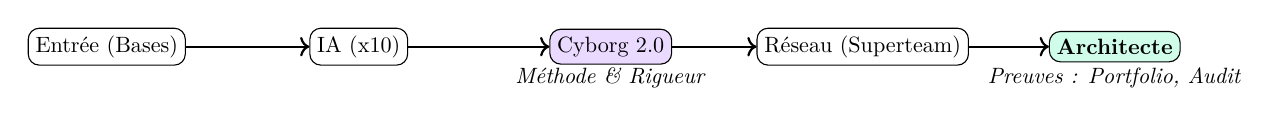
\begin{tikzpicture}[node distance=2cm, auto, scale=0.8, every node/.style={scale=0.8}]
        \node[draw, rectangle, rounded corners] (entree) {Entrée (Bases)};
        \node[draw, rectangle, rounded corners, right of=entree, xshift=2cm] (ia) {IA (x10)};
        \node[draw, rectangle, rounded corners, fill=SolanaPurple!20, right of=ia, xshift=2cm] (cyborg) {Cyborg 2.0};
        \node[draw, rectangle, rounded corners, right of=cyborg, xshift=2cm] (reseau) {Réseau (Superteam)};
        \node[draw, rectangle, rounded corners, fill=SolanaGreen!20, right of=reseau, xshift=2cm] (sortie) {\textbf{Architecte}};

        \draw[->, thick] (entree) -- (ia);
        \draw[->, thick] (ia) -- (cyborg);
        \draw[->, thick] (cyborg) -- (reseau);
        \draw[->, thick] (reseau) -- (sortie);

        \node[below of=cyborg, yshift=1cm, node distance=1.5cm] {\textit{Méthode \& Rigueur}};
        \node[below of=sortie, yshift=1cm, node distance=1.5cm] {\textit{Preuves : Portfolio, Audit}};
    \end{tikzpicture}
    \caption{La Chaîne de Valeur RBK 2.0}
\end{figure}

\section{Pourquoi RBK 2.0 ?}

RBK 2.0 répond à un décalage structurel entre l'offre éducative classique et les exigences d'architectes Web3 seniors : nous cadrons ici le "pourquoi" avant de détailler les sous-piliers.

\subsubsection{Diagnostic : L'Écart de Compétence (Skills Gap)}

Le fossé entre l'offre de formation classique et la demande du marché Web3 est béant.
\begin{enumerate}
    \item \textbf{Évaluation obsolète :} Les écoles notent la mémorisation; le marché paie la résolution de problèmes inconnus.
    \item \textbf{Absence de Sécurité :} La sécurité est souvent une option ou un module théorique. En Web3, c'est le prérequis absolu.
    \item \textbf{Pas de Production Réelle :} Les projets d'école finissent dans un dossier "brouillon". Un profil senior doit montrer un code en production.
    \item \textbf{Signaux Marché Faibles :} Un diplôme papier ne prouve rien à une DAO internationale. Seul le code (GitHub) et la réputation (On-chain) comptent.
\end{enumerate}

\subsubsection{Les Différenciateurs RBK 2.0}

\begin{itemize}
    \item \textbf{Méthodologie Cyborg 2.0} (voir Chap. 4) : Nous intégrons l'IA comme outil de base, pas comme aide à la triche.
    \item \textbf{Intensité 28 Semaines} (voir Chap. 5) : Une immersion totale nécessaire pour changer de mindset.
    \item \textbf{Preuve de Travail (Proof of Work)} (voir Chap. 11) : Chaque ligne de code contribue à un portfolio public auditable.
    \item \textbf{Réseau Global} : Connexion directe avec la Superteam et les opportunités internationales.
\end{itemize}

\subsubsection{Ce que RBK 2.0 n'est pas}

Il est crucial d'aligner les attentes. RBK 2.0 n'est :
\begin{itemize}
    \item \textbf{Pas un cours vidéo passif :} L'apprentissage se fait par la pratique douloureuse et gratifiante (Hard Fun).
    \item \textbf{Pas un bootcamp JavaScript :} Nous formons des ingénieurs système (Rust/Solidity), pas des développeurs frontend React (bien que ce soit une compétence annexe).
    \item \textbf{Pas une promesse magique :} L'ISA et le placement dépendent à 100\% de l'engagement de l'étudiant.
\end{itemize}

\begin{strategieBox}{Positionnement Stratégique}
RBK 2.0 est une "School of Engineering" accélérée, positionnée entre le bootcamp d'élite (type 42) et l'incubateur de startups Web3.
\end{strategieBox}

\subsubsection{Changement de Paradigme}

\begin{table}[H]
    \caption{Le Changement de Paradigme RBK 2.0 (Détaillé)}
    \centering
    \renewcommand{\arraystretch}{1.4} % Aère les lignes
    \rowcolors{2}{SolanaBlue!5}{white}
    \small % Augmentation de la taille de police (était \tiny)
    \begin{tabularx}{\textwidth}{|>{\bfseries}l|X|X|l|}
        \hline
        \rowcolor{SolanaPurple!20} \textbf{Dimension} & \textbf{Ancien Monde (Univ/Bootcamps)} & \textbf{RBK 2.0 (Senior-by-Design)} & \textbf{Signal Recruteur} \\
        \hline
        Objectif & Valider des modules & Livrer de la valeur & GitHub Activity \\
        Outils & Interdits (Pas d'IA) & Obligatoires (Cursor, Copilot) & Vitesse d'exécution \\
        Rythme & Linéaire, théorique & Cyclique, intense, pratique & Résilience \\
        Sécurité & Optionnelle / Théorique & \textbf{By Design (Audit Flow)} & Portfolio d'audits \\
        Santé & Ignorée & \textbf{Gérée (Protocole Anti-Burnout)} & Stabilité émotionnelle \\
        Sortie & Stage sous-payé & Consultance / CDI Senior / Grant & Contrats signés \\
        \hline
    \end{tabularx}
\end{table}


% 2. Analyse du Contexte
\chapter{ANALYSE DU CONTEXTE}
\label{chap:contexte}

\section{L'Opportunité Web3 \& Solana}

\subsubsection{Définitions Minimales (Lexique Opérationnel)}
Pour comprendre l'arbitrage RBK, il faut maîtriser le vocabulaire du marché :
\begin{itemize}
    \item \textbf{Web3 :} Un internet où les utilisateurs possèdent leurs données et leurs actifs, sécurisé par des réseaux décentralisés (Blockchains).
    \item \textbf{Solana (SVM) :} La blockchain la plus performante à ce jour (65k TPS théoriques), optimisée pour des applications grand public (Payments, Gaming, DePIN).
    \item \textbf{DeFi (Decentralized Finance) :} Services financiers (prêt, échange) sans intermédiaire bancaire.
    \item \textbf{DePIN (Decentralized Physical Infrastructure) :} Réseaux physiques (Wifi, GPU) gérés par des incitations crypto.
    \item \textbf{Bounty :} Mission à la tâche rémunérée en stablecoins\footnote{\textbf{Stablecoin :} Cryptomonnaie dont le cours est indexé sur une monnaie fiduciaire (ex: USDC = 1 Dollar USD) pour éviter la volatilité.} (USDC), souvent premier revenu d'un étudiant.
\end{itemize}

\subsubsection{Segmentation de la Demande}

Le marché ne cherche pas "un dev blockchain", mais des spécialistes par verticale.

\begin{table}[h]
    \caption{Segmentation des Rôles Web3 (2025)}
    \centering
    \small
    \rowcolors{2}{gray!5}{white}
    \begin{tabularx}{\textwidth}{l l X l}
        \toprule
        \textbf{Segment} & \textbf{Rôles Clés} & \textbf{Livrables Concrets} & \textbf{Compétence Dominante} \\
        \midrule
        \textbf{DeFi} & Smart Contract Eng. & AMM, Lending Protocol, Vaults & Mathématiques \& Sécurité \\
        \textbf{DePIN} & Rust Embedded Eng. & Drivers IoT, Proof-of-Coverage & Optimisation Bas-niveau \\
        \textbf{Infra} & DevOps / RPC Eng. & Indexers, Validators, Nodes & Linux, Docker, Rust \\
        \textbf{Consumer} & Mobile dApp Dev. & Wallet UI, Payment SDK & UX/UI, React Native \\
        \bottomrule
    \end{tabularx}
\end{table}

\subsubsection{Pourquoi Solana est un Accélérateur d'Employabilité}
Contrairement à Ethereum (EVM) qui est saturé et fragmenté (L2s), Solana offre un écosystème unifié et en hyper-croissance (+500\% d'adresses actives en 2024). Pour un junior, la courbe d'apprentissage est plus raide (Rust), mais la concurrence est moindre et les primes sont plus élevées. La \textbf{Superteam} offre un pipeline direct vers l'emploi via Earn.

\begin{tcolorbox}[colback=red!5!white,colframe=red!75!black,title=Market Intelligence – Q4 2025]
\begin{enumerate}
    \item \textbf{Postes ouverts :} 15~000+ offres actives en Remote Global\footnote{Source : Web3.career \& TrueUp Tech Jobs Report, Q4 2024.}.
    \item \textbf{Pénurie :} 58\% des Lead Techs citent le recrutement d'ingénieurs Rust seniors comme leur blocage n°1.
    \item \textbf{Développeurs Actifs :} < 25~000 développeurs crypto mensuels vs 25M devs Web2. L'opportunité d'arbitrage est de x1000\footnote{Source : Electric Capital Developer Report 2023.}.
\end{enumerate}
\end{tcolorbox}


\section{Dynamique Salariale}

\subsubsection{Hypothèses de Lecture (TND vs USD)}
Les chiffres présentés ci-dessous sont exprimés en USD brut annuel. Pour un talent tunisien en remote :
\begin{itemize}
    \item \textbf{Conversion :} 1 USD $\approx$ 3.1 TND.
    \item \textbf{Fiscalité :} En statut "Exportateur de Services" (entreprise totalement exportatrice), l'imposition est avantageuse, maximisant le net.
    \item \textbf{Réalité Marché :} Le salaire "Junior" Web3 (60k\$) correspond souvent à un salaire "VP Engineering" sur le marché local.
\end{itemize}

\subsubsection{Grille de Rémunération Standard}

\begin{table}[h]
    \caption{Grille Salariale Web3 (Remote Global) vs Local}
    \centering
    \rowcolors{2}{SolanaGreen!5}{white}
    \begin{tabularx}{\textwidth}{l c c l}
        \rowcolor{SolanaGreen} \textbf{Rôle} & \textbf{Junior (0-2 ans)} & \textbf{Senior (3+ ans)} & \textbf{Pré-requis} \\
        \toprule
        Solana Rust Engineer & 60k\$ - 90k\$ & 140k\$ - 220k\$ & Portfolio GitHub Solide \\
        Security Auditor & 80k\$ - 120k\$ & 250k\$+ & Track Record de vulnérabilités trouvées \\
        Fullstack dApp & 50k\$ - 80k\$ & 110k\$ - 160k\$ & Portfolio React + Anchor \\
        \textit{Dev Web2 (Tunisie)} & \textit{15k - 25k TND} & \textit{40k - 60k TND} & \textit{Diplôme Ingénieur} \\
        \bottomrule
    \end{tabularx}
    \footnotesize{\textit{Sources : Web3.career, Pantera Capital Salary Survey 2024. Note : Les montants Web3 sont en Brut Global. En Tunisie, grâce au statut exportateur (off-shore/startup act), le Net est maximisé (charges allégées), rendant le pouvoir d'achat x3 supérieur au local.}}
\end{table}

\subsubsection{Modèle ROI Candidat (Simulation 1 an)}

\begin{table}[h]
    \centering
    \small
    \begin{tabularx}{\textwidth}{|l|c|X|l|}
        \hline
        \textbf{Scénario} & \textbf{Revenu Cible} & \textbf{Time-to-Revenue} & \textbf{Risques} \\ \hline
        \textbf{Prudent} & 1 500 \$/mois & 4 mois post-cursus & Marché Bear, Anglais moyen \\ \hline
        \textbf{Médian} & 3 000 \$/mois & 2 mois post-cursus & Concurrence, Portfolio standard \\ \hline
        \textbf{Top Gun} & 5 000 \$/mois & Pendant le cursus (S20) & Burnout, Gestion charge travail \\ \hline
    \end{tabularx}
\end{table}


\section{Croissance du Marché}

\subsubsection{Définition de l'Index}
Le graphique ci-dessous agrège le volume d'offres d'emploi techniques (Engineering, Product, Design) postées sur les 5 principaux job boards crypto, normalisé sur une base 100 en Janvier 2021.

\subsubsection{Lecture Stratégique}
La corrélation avec le prix des actifs (BTC/SOL) diminue : les entreprises construisent (Build) même en bear market. Cela signifie que l'embauche se professionnalise et devient moins volatile. Pour RBK, cela valide la stratégie de "formation longue" (7 mois) qui lisse les cycles de court terme.

\begin{center}
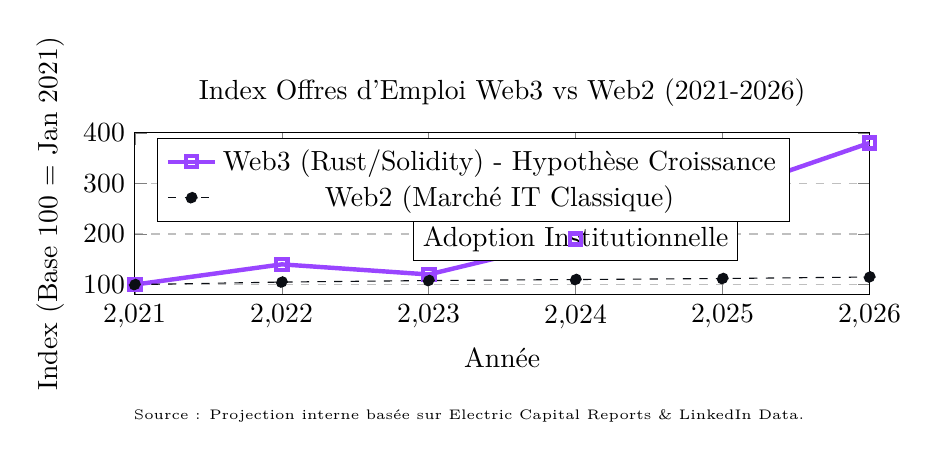
\begin{tikzpicture}
    \begin{axis}[
        title={Index Offres d'Emploi Web3 vs Web2 (2021-2026)},
        xlabel={Année},
        ylabel={Index (Base 100 = Jan 2021)},
        xmin=2021, xmax=2026,
        ymin=80, ymax=400,
        xtick={2021,2022,2023,2024,2025,2026},
        legend pos=north west,
        ymajorgrids=true,
        grid style=dashed,
        width=0.9\textwidth,
        height=0.3\textwidth
    ]
    
    \addplot[color=SolanaPurple, mark=square, ultra thick]
        coordinates {
        (2021,100)(2022,140)(2023,120)(2024,190)(2025,280)(2026,380)
        };
        \addlegendentry{Web3 (Rust/Solidity) - Hypothèse Croissance}
        
    \addplot[color=BaseDark, mark=*, dashed]
        coordinates {
        (2021,100)(2022,105)(2023,108)(2024,110)(2025,112)(2026,115)
        };
        \addlegendentry{Web2 (Marché IT Classique)}
        
    \node[draw, fill=white] at (axis cs: 2024, 190) {Adoption Institutionnelle};
        
    \end{axis}
    \node[anchor=north, font=\tiny] at (current bounding box.south) {Source : Projection interne basée sur Electric Capital Reports \& LinkedIn Data.};
\end{tikzpicture}
\end{center}


% 3. Arbitrage Technologique
\chapter{ARBITRAGE TECHNOLOGIQUE}
\label{chap:arbitrage}

\section{Solana vs EVM : Le Choix Stratégique}

\begin{ceoBox}{L'Arbitrage en un coup d'œil}
Pour un dirigeant, le choix technologique se résume ainsi :
\begin{itemize}
    \item \textbf{Solana (SVM)} : Optimisé pour la \textbf{vitesse} et le \textbf{coût infime}. Idéal pour les applications grand public (Paiements, Jeux, DePIN). C'est le "Nasdaq" de la blockchain.
    \item \textbf{Ethereum (EVM)} : Optimisé pour la \textbf{sécurité} et la \textbf{décentralisation}. Idéal pour la finance lourde et les actifs de haute valeur. C'est le "Coffre-fort" numérique.
\end{itemize}
\textbf{Notre approche :} Former sur l'architecture la plus exigeante (Solana/Rust) rend l'apprentissage de la seconde (Ethereum/Solidity) trivial.
\end{ceoBox}

\subsubsection{Méthode d'Arbitrage (Scoring)}
Notre choix technologique n'est pas idéologique, il est pragmatique. Nous évaluons les écosystèmes selon trois vecteurs pondérés :

\begin{itemize}
    \item \textbf{Employabilité (Poids 50\%) :} Volume d'offres, niveau des salaires, pénurie relative.
    \item \textbf{Innovation (Poids 30\%) :} Capacité à supporter de nouveaux cas d'usage (DePIN, Mobile).
    \item \textbf{Stabilité (Poids 20\%) :} Maturité des outils (Tooling), documentation, risque de fork.
\end{itemize}

Actuellement, Solana domine sur l'Innovation et la pénurie de talents, tandis qu'EVM domine sur la stabilité et le volume total de TVL.

\subsubsection{Conséquences Pédagogiques : "Solana-first, EVM-competent"}
Apprendre Rust (Solana) est plus difficile que Solidity (EVM) en raison de la gestion de la mémoire et de la concurrence. C'est pourquoi nous commençons par le plus dur :
\begin{enumerate}
    \item \textbf{Phase 0-1 (Rust) :} L'étudiant acquiert une rigueur système (Memory safety, Type system).
    \item \textbf{Phase 2 (Solidity) :} Le passage à l'EVM est vécu comme une simplification, permettant de se concentrer sur les failles de sécurité spécifiques (Re-entrancy) plutôt que sur la syntaxe.
\end{enumerate}

\subsubsection{Risque Technologique et Atténuation}
Le risque principal de Solana est sa jeunesse (pannes historiques, changements d'API). Nous l'atténuons par une veille technique active et l'utilisation de wrappers stables (Anchor). Le risque EVM est la fragmentation (L2s\footnote{\textbf{L2 (Layer 2) / Rollup :} Technologies (comme Arbitrum, Optimism) qui s'exécutent "au-dessus" d'une blockchain principale (L1) pour traiter les transactions plus vite et moins cher, tout en héritant de sa sécurité.} incompatibles) ; nous l'adressons en enseignant les standards (ERC-20, ERC-721) qui restent universels.

\subsubsection{Matrice Comparative Détaillée}

\begin{table}[h]
    \caption{Comparatif Technique et Stratégique (2025)}
    \centering
    \small
    \rowcolors{2}{SolanaBlue!5}{white}
    \begin{tabularx}{\textwidth}{L X X l}
        \rowcolor{SolanaPurple!20} \textbf{Critère} & \textbf{Ethereum/EVM} & \textbf{Solana/SVM} & \textbf{RBK Posture} \\
        \toprule
        \textbf{Modèle Mental} & Séquentiel (Single Thread) & Parallèle (Sealevel) & Maîtrise des deux \\
        \textbf{Langage} & Solidity (Haut niveau) & Rust (Système) & Rust comme fondation \\
        \textbf{Coût Tx} & 2\$ - 50\$ (L1) / 0.1\$ (L2) & < 0.0001\$ & Optimisation Gas \\
        \textbf{Sécurité} & Surface d'attaque mature & Surface complexe (CPI) & Audit First \\
        \textbf{Opportunité} & Corporate / Audit & Startup / Growth & Polyvalence \\
        \bottomrule
    \end{tabularx}
\end{table}

\section{Stratégie Multi-Chain \& Interopérabilité}

\subsubsection{Interopérabilité : Notions Essentielles}
L'avenir n'est pas "Winner Takes All", mais "Cross-Chain"\footnote{\textbf{Cross-Chain :} Architecture permettant l'interopérabilité et la communication entre des blockchains indépendantes, essentielle pour éviter les silos de liquidité.}. Un architecte doit comprendre comment déplacer de la valeur et de l'information entre des réseaux hétérogènes.
\begin{itemize}
    \item \textbf{Bridge (Lock \& Mint)}\footnote{\textbf{Bridge :} Protocole ou infrastructure permettant de transférer des actifs (Tokens) d'une blockchain à une autre.} : Verrouiller un actif sur la chaîne A pour en créer une représentation sur la chaîne B.
    \item \textbf{Messaging (General Passing) :} Envoyer une instruction arbitraire d'une chaîne à l'autre (ex: Vote DAO sur Eth -> Exécution sur Sol).
    \item \textbf{Finality :} Le temps nécessaire pour garantir qu'une transaction ne sera jamais annulée (Solana: ~400ms, Eth: ~12min).
\end{itemize}

\subsubsection{Risques Cross-Chain}
Les "Bridges" sont historiquement les cibles les plus hackées (>2 Mrd\$ volés). RBK enseigne une posture paranoïaque :
\begin{enumerate}
    \item Ne jamais faire confiance à un validateur unique.
    \item Vérifier les preuves cryptographiques (Merkle Proofs).
    \item Utiliser des standards audités (Wormhole, LayerZero) plutôt que des solutions maison.
\end{enumerate}

\subsubsection{Livrables Étudiants}
Pour valider le module interopérabilité, l'étudiant doit livrer :
\begin{itemize}
    \item Un schéma d'architecture cross-chain (flux des actifs).
    \item Une implémentation de transfert de message (ex: "Hello World" cross-chain).
    \item Une analyse des risques spécifiques à son architecture.
\end{itemize}

\begin{figure}[h]
    \centering
    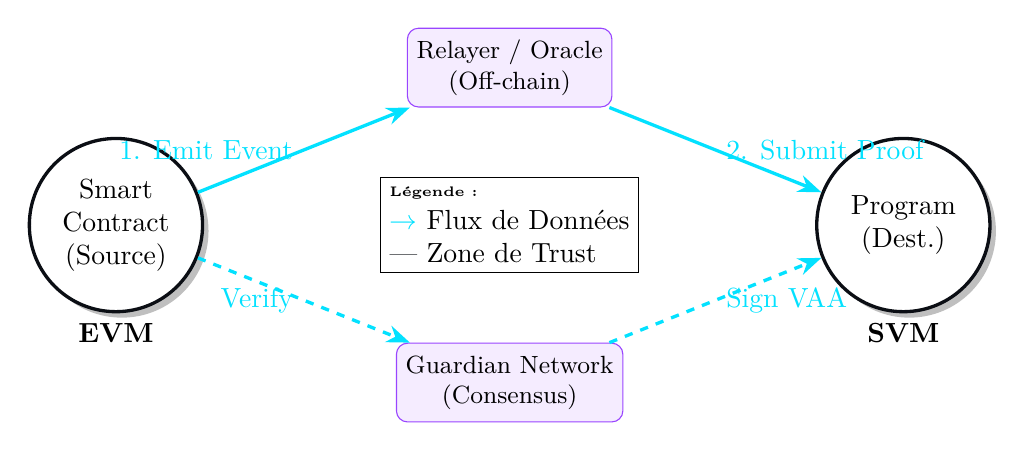
\begin{tikzpicture}[
        node distance=2.5cm,
        chain/.style={circle, draw=BaseDark, very thick, fill=white, minimum size=2.2cm, align=center, drop shadow},
        component/.style={rectangle, draw=SolanaPurple, fill=SolanaPurple!10, rounded corners, minimum width=2.5cm, minimum height=1cm, align=center, font=\small},
        link/.style={->, >=Stealth, very thick, SolanaBlue}
    ]
        % Zones
        \node[chain, label=below:\textbf{EVM}] (evm) at (0,0) {Smart\\Contract\\(Source)};
        \node[chain, label=below:\textbf{SVM}] (svm) at (10,0) {Program\\(Dest.)};
        
        % Bridge Components
        \node[component] (relayer) at (5, 2) {Relayer / Oracle\\(Off-chain)};
        \node[component] (guardian) at (5, -2) {Guardian Network\\(Consensus)};
        
        % Flows
        \draw[link] (evm) -- node[midway, left] {1. Emit Event} (relayer);
        \draw[link] (relayer) -- node[midway, right] {2. Submit Proof} (svm);
        \draw[link, dashed] (evm) -- node[midway, left] {Verify} (guardian);
        \draw[link, dashed] (guardian) -- node[midway, right] {Sign VAA} (svm);
        
        % Legend
        \node[draw, fill=white, align=left] at (5,0) {\tiny \textbf{Légende :}\\ \textcolor{SolanaBlue}{$\rightarrow$} Flux de Données\\ \textcolor{BaseDark}{---} Zone de Trust};

    \end{tikzpicture}
    \caption{Architecture Cross-Chain : Flux de Vérification}
\end{figure}


% 4. Méthodologie Cyborg 2.0
\chapter{MÉTHODOLOGIE CYBORG 2.0}
\label{chap:methodologie}

\section{Philosophie Pédagogique : Intégration du Bien-être}

La méthodologie RBK 2.0 ne se contente pas de former des techniciens ; elle forge des \textit{athlètes cognitifs}. Conscients de la charge mentale intense imposée par l'apprentissage du développement blockchain (Rust, Zero-Knowledge Proofs, audits de sécurité), nous avons intégré une dimension \textbf{santé mentale et résilience} au cœur même du curriculum.

\begin{figure}[H]
    \centering
    \begin{tikzpicture}[
        scale=0.9,
        every node/.style={scale=0.9},
        day/.style={rectangle, draw=SolanaPurple, fill=white, rounded corners, minimum width=2.5cm, minimum height=3cm, align=center, drop shadow},
        arrow/.style={->, >=Stealth, thick, SolanaBlue},
        label/.style={font=\bfseries\small, color=BaseDark}
    ]
        % Nodes
        \node[day] (lundi) at (0,0) {\textbf{LUNDI}\\\footnotesize Planning\\Stratégique\\\faBrain\ Focus};
        \node[day] (mardi) at (3.5,0) {\textbf{MARDI}\\\footnotesize Deep Work\\(IA Assisted)\\\faLaptopCode\ Dev};
        \node[day] (mercredi) at (7,0) {\textbf{MERCREDI}\\\footnotesize Pair\\Programming\\\faUserFriends\ Collab};
        \node[day] (jeudi) at (10.5,0) {\textbf{JEUDI}\\\footnotesize Audit \&\\Review\\\faBug\ Quality};
        \node[day] (vendredi) at (14,0) {\textbf{VENDREDI}\\\footnotesize Débrief \&\\Resilience\\\faHeartbeat\ Santé};

        % Arrows
        \draw[arrow] (lundi) -- (mardi);
        \draw[arrow] (mardi) -- (mercredi);
        \draw[arrow] (mercredi) -- (jeudi);
        \draw[arrow] (jeudi) -- (vendredi);

        % Brace
        \draw[decorate, decoration={brace, amplitude=10pt}, thick, color=SolanaGreen] (0,1.7) -- (14,1.7) node[midway, above=15pt, color=SolanaGreen, font=\bfseries] {CYCLE HEBDOMADAIRE "SUSTAINABLE PERFORMANCE"};

    \end{tikzpicture}
    \caption{Le Cycle Hebdomadaire RBK 2.0}
\end{figure}

\subsubsection{Le Contrat de Performance Durable}
Nous imposons un cadre strict pour éviter le surmenage :
\begin{enumerate}
    \item \textbf{Deep Work Timeboxé :} Maximum 6 heures de code pur par jour. Au-delà, la productivité et la qualité du code chutent (bugs).
    \item \textbf{No-Code Weekend :} Interdiction de pousser du code sur GitHub du samedi 12h au lundi 8h (sauf Hackathon exceptionnel).
    \item \textbf{Rituel de Décompression :} Session de sport ou méditation obligatoire le vendredi après-midi.
\end{enumerate}

\subsubsection{Cadre d'Usage de l'IA (Cyborg Policy)}
L'IA est un levier, pas une béquille. Son usage est régulé :

\paragraph{Niveau 0 (Piscine) : Interdiction Totale}
L'étudiant doit développer ses modèles mentaux sans assistance. Copilot est désactivé. Toute détection de code généré entraîne une disqualification.

\paragraph{Niveau 1+ (Cursus) : Assistance Supervisée}
L'IA est autorisée pour :
\begin{itemize}
    \item Générer des tests unitaires (TDD).
    \item Expliquer des messages d'erreur obscurs.
    \item Produire du boilerplate (structs, imports).
\end{itemize}
Elle est \textbf{interdite} pour :
\begin{itemize}
    \item Résoudre l'exercice à la place de l'étudiant.
    \item Générer la logique core sans audit manuel ligne par ligne.
\end{itemize}

\section{Le Standard Studio : Excellence Opérationnelle}

RBK simule un environnement de travail "Production-Grade" dès la semaine 1.

\subsection{Definition of Done (DoD)}
Aucune tâche n'est validée sans respecter ces critères :
\begin{enumerate}
    \item \textbf{Code :} Fonctionnel, formatté (`cargo fmt`), sans warnings.
    \item \textbf{Tests :} Tests unitaires passants + 1 Test d'intégration critique.
    \item \textbf{Compil :} Pipeline CI (GitHub Actions) au vert.
    \item \textbf{Doc :} README à jour (Install, Run, Test).
\end{enumerate}

\subsection{Rituels "Agile Web3"}
\begin{itemize}
    \item \textbf{Daily Stand-up (Async)} : Status update sur Discord (Blockers/Progress).
    \item \textbf{Weekly Incident Drill} : Simulation de hack (le jeudi), post-mortem obligatoire.
    \item \textbf{Demo Day (Vendredi)} : Présentation produit (pas de slides, code only) 5 min.
\end{itemize}

\section{La « Piscine » Rust : Programme Pré-Piscine}

Pour maximiser les chances de succès et réduire le taux d'abandon, RBK 2.0 intègre une phase préparatoire structurée.

\subsubsection{Objectif : Filtrer la Rigueur}
La Piscine Rust n'évalue pas le niveau informatique initial (nous acceptons les débutants brillants), mais la capacité d'apprentissage rapide et la résilience à l'échec. C'est un test de caractère.

\subsubsection{Rubrique d'Évaluation (Scoring)}
Nous utilisons une grille précise pour objectiver la sélection :

\begin{table}[H]
    \caption{Critères de Sélection Pré-Piscine}
    \centering
    \small
    \rowcolors{2}{SolanaBlue!5}{white}
    \begin{tabularx}{\textwidth}{l X c c}
        \toprule
        \textbf{Critère} & \textbf{Description} & \textbf{Poids} & \textbf{Seuil Min.} \\
        \midrule
        \textbf{Rustlings} & Complétion des 80 exercices de syntaxe & 30\% & 100\% \\
        \textbf{Algo (Codewars)} & Résolution de problèmes logiques (Katas) & 30\% & Rank 5kyu \\
        \textbf{Git Hygiene} & Qualité des commits (Atomicité, Messages) & 20\% & Pro \\
        \textbf{Discipline} & Régularité des pushs (Green Dots) & 20\% & Quotidien \\
        \bottomrule
    \end{tabularx}
\end{table}

\subsubsection{Anti-Triche et Preuve de Travail}
Pour garantir que c'est bien l'étudiant qui code :
\begin{itemize}
    \item \textbf{Entretiens Flash :} Le mentor demande d'expliquer une ligne de code aléatoire en direct.
    \item \textbf{Live Coding :} Une épreuve finale surveillée (proctored) sans IA.
    \item \textbf{Analyse Stylométrique :} Détection des changements brusques de style de code (indiquant un copier-coller).
\end{itemize}

\section{Protocole Anti-Burnout}

Nous avons industrialisé la protection de nos étudiants via un protocole strict.

\subsubsection{Monitoring Hebdomadaire}
Chaque vendredi, les étudiants remplissent un "Wellness Check" anonymisé de 5 questions :
\begin{enumerate}
    \item Qualité du sommeil (1-5).
    \item Niveau de stress perçu (1-5).
    \item Sentiment de compétence (Impostor Syndrome) (1-5).
\end{enumerate}

\subsubsection{Seuils et Escalade (Traffic Light Protocol)}

\begin{table}[H]
    \caption{Matrice d'Intervention Santé Mentale}
    \centering
    \small
    \rowcolors{2}{red!5}{white}
    \begin{tabularx}{\textwidth}{l X l l}
        \toprule
        \textbf{Zone} & \textbf{Critère Déclencheur} & \textbf{Action Immédiate} & \textbf{Responsable} \\
        \midrule
        \textbf{\textcolor{green}{VERT}} & Score > 4/5 & Rien à signaler & Mentor \\
        \textbf{\textcolor{orange}{ORANGE}} & Score < 3/5 ou Retard livrables & Entretien 1-on-1 & Student Success \\
        \textbf{\textcolor{red}{ROUGE}} & Score < 2/5 ou "Panic Attack" & \textbf{Arrêt forcé 48h} & Head of Ed \\
        \bottomrule
    \end{tabularx}
\end{table}

\subsubsection{Plan de Remédiation}
En cas de zone rouge persistante, nous activons la "Pause Fusible" :
\begin{itemize}
    \item \textbf{Semaine Off :} L'étudiant coupe tout écran pendant 7 jours sans pénalité.
    \item \textbf{Rattrapage :} Il réintègre la cohorte avec un plan allégé ou bascule sur la cohorte suivante (Roll-over) si nécessaire.
\end{itemize}

\begin{figure}[H]
    \centering
    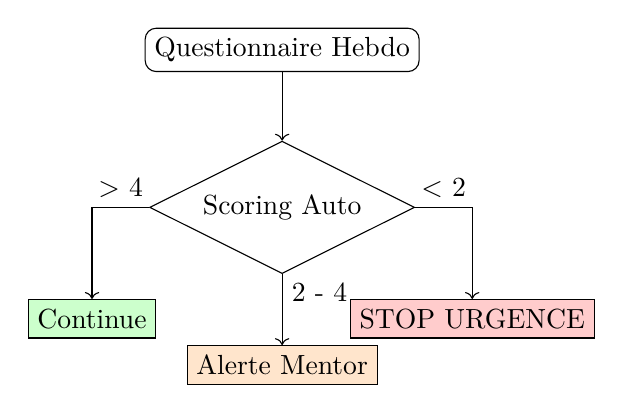
\begin{tikzpicture}[scale=0.8, node distance=2cm]
        \node[draw, rectangle, rounded corners] (quest) {Questionnaire Hebdo};
        \node[draw, diamond, aspect=2, below of=quest] (score) {Scoring Auto};
        \node[draw, rectangle, fill=green!20, below left of=score, xshift=-1cm] (ok) {Continue};
        \node[draw, rectangle, fill=orange!20, below of=score] (warn) {Alerte Mentor};
        \node[draw, rectangle, fill=red!20, below right of=score, xshift=1cm] (stop) {STOP URGENCE};

        \draw[->] (quest) -- (score);
        \draw[->] (score) -| node[near start, above] {> 4} (ok);
        \draw[->] (score) -- node[near start, right] {2 - 4} (warn);
        \draw[->] (score) -| node[near start, above] {< 2} (stop);
    \end{tikzpicture}
    \caption{Algorithme de Décision Anti-Burnout}
\end{figure}


% 5. Structure du Cursus
\chapter{STRUCTURE DU CURSUS}
\label{chap:structure}

\section{Architecture Cursus : 28 Semaines}

\subsubsection{Vue d'Ensemble : Phases et Objectifs}
\textbf{28 semaines au total = 24 semaines techniques + 4 semaines de professionnalisation.}

Le cursus est une séquence logique de déconstruction et reconstruction des compétences.
\begin{enumerate}
    \item \textbf{Phase 0 (Piscine) :} Nettoyer les mauvaises habitudes. \textit{Livrable : CLI Tool en Rust.}
    \item \textbf{Phase 1 (Fondations) :} Maîtriser les briques bas-niveau. \textit{Livrable : Token standard \& Swap.}
    \item \textbf{Phase 2 (Spécialisation) :} Devenir expert sur une stack (Solana/EVM/Product). \textit{Livrable : Protocole DeFi ou Dashboard.}
    \item \textbf{Phase 3 (Professionnalisation) :} Livrer un produit fini. \textit{Livrable : Capstone audité.}
\end{enumerate}

\section{Découpage Commercial : 3 Niveaux Stackables}

Pour maximiser l'accessibilité et la réussite, le cursus de 28 semaines est découpé en 3 niveaux certifiants et indépendants ("Stackable"). Ce modèle permet aux étudiants de valider des jalons intermédiaires, de réduire le risque financier, et de ne s'engager sur la suite qu'après avoir prouvé leur compétence. Chaque niveau délivre une valeur tangible immédiate : une compétence technique, une preuve vérifiable (SBT), et un accès réseau. L'étudiant peut s'arrêter après le N1 avec un profil junior employable, ou continuer pour viser l'excellence "Studio".

\begin{figure}[h]
    \centering
    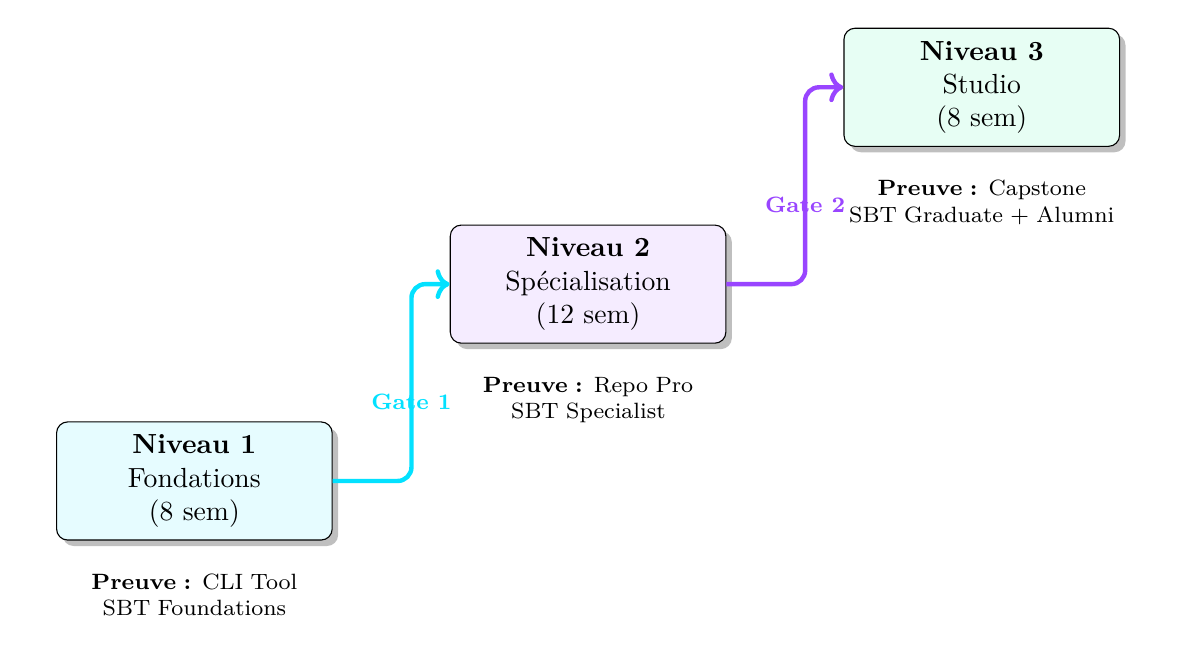
\begin{tikzpicture}[node distance=1.5cm, auto]
        % Nodes (Boîtes) - Espacement horizontal augmenté (0 -> 5 -> 10)
        \node[draw, fill=SolanaBlue!10, rounded corners, minimum width=3.5cm, minimum height=1.5cm, align=center, drop shadow] (n1) at (0,0) {\textbf{Niveau 1}\\Fondations\\(8 sem)};
        \node[draw, fill=SolanaPurple!10, rounded corners, minimum width=3.5cm, minimum height=1.5cm, align=center, drop shadow] (n2) at (5,2.5) {\textbf{Niveau 2}\\Spécialisation\\(12 sem)};
        \node[draw, fill=SolanaGreen!10, rounded corners, minimum width=3.5cm, minimum height=1.5cm, align=center, drop shadow] (n3) at (10,5) {\textbf{Niveau 3}\\Studio\\(8 sem)};
        
        % Flèches (Chemin en escalier propre : Sortie Est -> Montée -> Entrée Ouest)
        \draw[->, ultra thick, SolanaBlue, rounded corners=5pt] (n1.east) -- ++(1,0) |- (n2.west) node[pos=0.25, below, font=\footnotesize\bfseries] {Gate 1};
        \draw[->, ultra thick, SolanaPurple, rounded corners=5pt] (n2.east) -- ++(1,0) |- (n3.west) node[pos=0.25, below, font=\footnotesize\bfseries] {Gate 2};
        
        % Labels Preuves (Ancrés proprement sous les nœuds)
        \node[below=0.3cm of n1, font=\footnotesize, align=center, text width=4cm] {\textbf{Preuve :} CLI Tool\\SBT Foundations};
        \node[below=0.3cm of n2, font=\footnotesize, align=center, text width=4cm] {\textbf{Preuve :} Repo Pro\\SBT Specialist};
        \node[below=0.3cm of n3, font=\footnotesize, align=center, text width=4cm] {\textbf{Preuve :} Capstone\\SBT Graduate + Alumni};
    \end{tikzpicture}
    \caption{Staircase de Progression (3 Niveaux). \textit{Les "Gates" symbolisent des examens de passage obligatoires conditionnant l'accès au niveau supérieur.}}
\end{figure}

\begin{tcolorbox}[colback=gray!5,colframe=gray!50,title=Passerelles d'Admission]
L'entrée directe en Niveau 2 ou 3 est possible pour les candidats expérimentés, sous réserve de réussite aux \textbf{Tests de Positionnement} (voir Annexe G).
\end{tcolorbox}

\begin{table}[h]
    \caption{Structure Stackable}
    \centering
    \small
    \rowcolors{2}{gray!5}{white}
    \begin{tabularx}{\textwidth}{|l|l|l|X|l|}
        \hline
        \textbf{Niveau} & \textbf{Durée} & \textbf{Pré-requis} & \textbf{Preuves Attendues} & \textbf{Sortie} \\ \hline
        \textbf{1. Fondations} & 8 Sem. & Débutant (Motivé) & CLI Rust, Audit Trail, Mini-App & SBT Fundamentals \\ \hline
        \textbf{2. Track} & 12 Sem. & Gate 1 (ou Test) & DApp Complexe, Tests E2E, CI/CD & SBT Specialist \\ \hline
        \textbf{3. Studio} & 8 Sem. & Gate 2 (ou Portfolio) & Capstone Audité, Demo Publique & SBT Graduate \\ \hline
    \end{tabularx}
\end{table}

Le Chapitre 6 détaille l'exécution opérationnelle de ces phases semaine par semaine.

\subsubsection{Definition of Done (DoD) par Phase}
Pour passer à la phase suivante (Gate), l'étudiant doit prouver sa compétence.

\begin{table}[h]
    \caption{Definition of Done (DoD) et Gates de Passage}
    \centering
    \small
    \rowcolors{2}{SolanaBlue!5}{white}
    \begin{tabularx}{\textwidth}{l X X c}
        \toprule
        \textbf{Phase} & \textbf{Livrable Pivot} & \textbf{Critère Qualité} & \textbf{Gate Score} \\
        \midrule
        \textbf{Ph. 0} & Rust CLI (grep-like) & Exécutable, Zéro warning, Tests unitaires & > 80/100 \\
        \textbf{Ph. 1} & Déploiement Token & Vérifiable sur Explorer, Script de mint & > 70/100 \\
        \textbf{Ph. 2} & Protocole Complexe & Architecture propre, Gas optimized & > 3 PRs validées \\
        \textbf{Ph. 3} & Capstone Mainnet & Audit de sécurité passé (sans Critical) & Note > 12/20 \\
        \bottomrule
    \end{tabularx}
\end{table}

\subsubsection{Système de Validation et Rattrapage}
Le scoring est une moyenne pondérée : \textbf{Technique (60\%)}, \textbf{Soft Skills (20\%)}, \textbf{Discipline (20\%)}.
\begin{itemize}
    \item \textbf{Score > 70/100 :} Passage automatique (GO).
    \item \textbf{Score 50-70 :} Passage conditionnel (WARN). Rattrapage obligatoire sous 2 semaines.
    \item \textbf{Score < 50 :} Redoublement ou réorientation (NO-GO).
\end{itemize}

\subsubsection{Charge de Travail et Discipline d'Exécution}
Le rythme est intense. Une semaine type représente 40 à 50 heures d'engagement.

\begin{table}[h]
    \caption{Rituel Hebdomadaire et Livrables}
    \centering
    \small
    \rowcolors{2}{gray!5}{white}
    \begin{tabularx}{\textwidth}{l X l}
        \toprule
        \textbf{Moment} & \textbf{Sortie Attendue} & \textbf{Outil} \\
        \midrule
        Lun. Matin & Planification des tâches (Issues) & GitHub Projects \\
        Mar. - Jeu. & Code, Tests, Commits (Deep Work) & VS Code / Cursor \\
        Ven. Midi & Pull Request (PR) pour review & GitHub \\
        Ven. PM & Demo Video (Loom) & Loom / Discord \\
        \bottomrule
    \end{tabularx}
\end{table}

\begin{figure}[h]
    \centering
    \begin{tikzpicture}[
        node distance=0.8cm,
        phase/.style={rectangle, draw=none, fill=SolanaPurple!10, rounded corners, minimum width=13cm, minimum height=1.5cm, align=left, text width=12cm, drop shadow},
        title/.style={font=\bfseries\large, color=SolanaPurple},
        detail/.style={font=\small\color{BaseDark}},
        arrow/.style={->, >=Stealth, ultra thick, SolanaGreen}
    ]
        \node[phase] (phase1) {\textbf{\color{SolanaPurple}NIVEAU 1 : FONDATIONS (8 Semaines)}\\ \footnotesize Piscine Rust (4s) + Fondations Web3 (4s). Gate: Mini-DApp & CLI};
        
        \node[phase, below=of phase1] (phase2) {\textbf{\color{SolanaPurple}NIVEAU 2 : SPÉCIALISATION (12 Semaines)}\\ \footnotesize Track A (Solana) / B (EVM) / C (Product). Gate: Protocole Complexe};
        
        \node[phase, below=of phase2] (phase3) {\textbf{\color{SolanaPurple}NIVEAU 3 : PROFESSIONNALISATION (8 Semaines)}\\ \footnotesize Capstone Studio (4s) + Audit & Carrière (4s). Gate: Mainnet Launch};

        \draw[arrow] (phase1) -- (phase2);
        \draw[arrow] (phase2) -- (phase3);

    \end{tikzpicture}
    \caption{Architecture Temporelle Alignée (24 Sem. Tech + 4 Sem. Carrière = 28 Semaines)}
\end{figure}

\section{Track C : Web3 Product \& Ecosystem Strategy}

\subsubsection{Positionnement Stratégique}
Le Track C forme les "Product Owners" et "Token Designers" qui manquent aux équipes techniques. Ils ne codent pas le smart contract, mais ils en définissent la logique économique et gouvernent son déploiement. Ils travaillent en binôme avec les étudiants du Track A/B. \textbf{Exemple de mission :} Concevoir le modèle d'inflation décroissante d'un stablecoin ou rédiger le Whitepaper technique d'un protocole DeFi.

\subsubsection{Livrables Track C (Portfolio)}
Pour valider ce track, l'étudiant doit produire 4 pièces maîtresses :
\begin{enumerate}
    \item \textbf{Tokenomics Paper :} Modélisation des incitations (Supply, Emission, Utility) simulée sur Machinations.io.
    \item \textbf{GTM Playbook :} Stratégie d'acquisition utilisateurs pour les 4 premières semaines post-launch.
    \item \textbf{Analytics Dashboard :} Un tableau de bord Dune Analytics monitorant les KPIs d'un protocole réel.
    \item \textbf{Governance Framework :} Les règles de la DAO (Quorum, Timelock, Voting power).
\end{enumerate}

\subsubsection{Plan de Progression (12 Semaines)}

\begin{table}[h]
    \caption{Syllabus Détaillé Track C}
    \centering
    \small
    \rowcolors{2}{SolanaBlue!5}{white}
    \begin{tabularx}{\textwidth}{l X l}
        \toprule
        \textbf{Module} & \textbf{Focus} & \textbf{Livrable Clé} \\
        \midrule
        \textbf{M1 : Product} & User Research, Prototyping (Figma) & PRD (Product Req. Doc) \\
        \textbf{M2 : Eco-Design} & Token Engineering, Game Theory & Simulation Excel/Python \\
        \textbf{M3 : Growth} & Community Building (Discord), Questing & Campagne Galxe \\
        \textbf{M4 : Ops \& Legal} & DAO Tooling (Realms), Compliance & Risk Memo \\
        \bottomrule
    \end{tabularx}
\end{table}

\begin{center}
    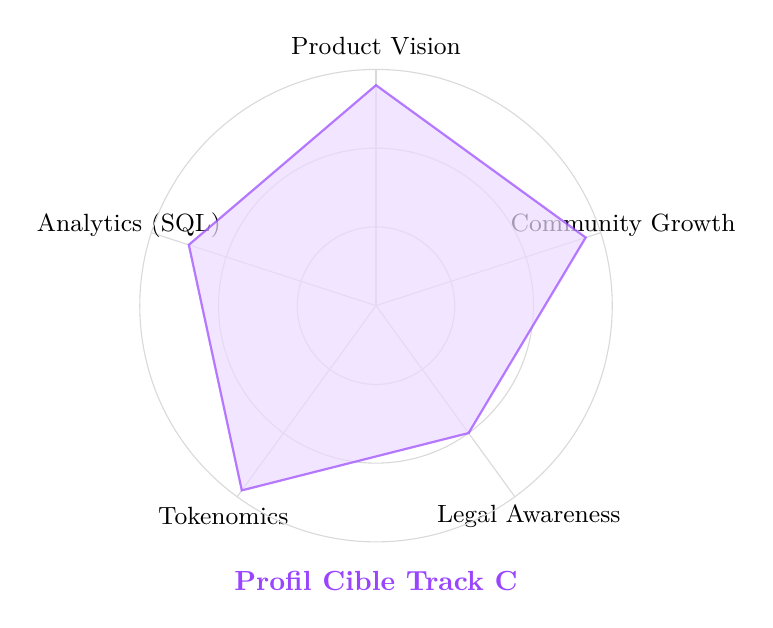
\begin{tikzpicture}
        \foreach \angle/\label in {90/Product Vision, 162/Analytics (SQL), 234/Tokenomics, 306/Legal Awareness, 18/Community Growth} {
            \draw[gray!30] (0,0) -- (\angle:3cm);
            \node at (\angle:3.3cm) {\small \label};
        }
        \draw[gray!30] (0,0) circle (1cm);
        \draw[gray!30] (0,0) circle (2cm);
        \draw[gray!30] (0,0) circle (3cm);
        
        \draw[SolanaPurple, thick, fill=SolanaPurple!20, opacity=0.7] 
        (90:2.8) -- (162:2.5) -- (234:2.9) -- (306:2.0) -- (18:2.8) -- cycle;
        
        \node[color=SolanaPurple, font=\bfseries] at (0,-3.5) {Profil Cible Track C};
    \end{tikzpicture}
\end{center}

\section{Certifications Industrielles \& Partenariats}

\subsection{Partenariat Solana Foundation : Accréditation "Developer Bootcamp"}
\begin{itemize}
    \item \textbf{Objectif} : Devenir le centre agréé de référence pour l'Afrique francophone.
    \item \textbf{Avantages} : Accès aux bourses (grants), certifications officielles (NFTs), et visibilité réseau.
\end{itemize}

\subsection{Certification "RBK Auditor"}
Reconnue par l'industrie pour sa rigueur.
\begin{enumerate}
    \item \textbf{Niveau 1 (Théorique)} : Examen sur les vulnérabilités (SWC Registry).
    \item \textbf{Niveau 2 (Pratique)} : CTF (Capture The Flag) et Audit d'un protocole réel.
    \item \textbf{Valeur} : Pipeline de recrutement direct avec des firmes d'audit partenaires.
\end{enumerate}

\subsection{Badges "Web3 Professional"}
Utilisation du standard \textbf{Open Badges 3.0} pour des preuves de compétences vérifiables sur LinkedIn.



% 6. Syllabus Technique Complet
\chapter{SYLLABUS TECHNIQUE COMPLET (48 SEMAINES)}

\textit{Note : Ce chapitre détaille l'exécution technique. L'intégration des Soft Skills (S45-S48) est traitée au Chapitre 7.}

\section{Calendrier Pédagogique Global}

\begin{figure}[H]
	\centering
	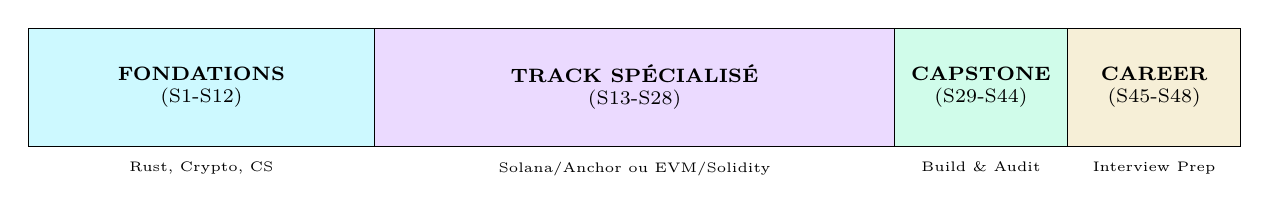
\begin{tikzpicture}[xscale=0.55, every node/.style={font=\scriptsize, align=center}]
		% Hauteur des blocs augmentée à 1.5cm pour tenir sur 2 lignes
		\draw[fill=SolanaBlue!20] (0,0) rectangle (8,1.5) node[midway] {\textbf{FONDATIONS}\\(S1-S12)};
		\draw[fill=SolanaPurple!20] (8,0) rectangle (20,1.5) node[midway] {\textbf{TRACK SPÉCIALISÉ}\\(S13-S28)};
		\draw[fill=SolanaGreen!20] (20,0) rectangle (24,1.5) node[midway] {\textbf{CAPSTONE}\\(S29-S44)};
		\draw[fill=MF_Gold!20] (24,0) rectangle (28,1.5) node[midway] {\textbf{CAREER}\\(S45-S48)};

		% Descriptions sous les blocs
		\node[below=2pt] at (4,0) {\tiny Rust, Crypto, CS};
		\node[below=2pt] at (14,0) {\tiny Solana/Anchor ou EVM/Solidity};
		\node[below=2pt] at (22,0) {\tiny Build \& Audit};
		\node[below=2pt] at (26,0) {\tiny Interview Prep};
	\end{tikzpicture}
	\caption{Timeline Macro du Cursus}
\end{figure}

\begin{center}\colorbox{SolanaBlue!20}{\parbox{\textwidth}{\centering \Large \textbf{NIVEAU 1 : PISCINE \& FONDATIONS (S1-S12)}}}\end{center}

\section{TRONC COMMUN : LA FORGE (S1-S12)}

\begin{table}[H]
	\caption{Synthèse Macro N1}
	\centering
	\small
	\rowcolors{2}{SolanaBlue!5}{white}
	\begin{tabularx}{\textwidth}{l X X l}
		\toprule
		\textbf{Sem.} & \textbf{Focus Technique} & \textbf{Livrable Pivot}      & \textbf{Gate Qualité} \\
		\midrule
		S1            & OS \& Git Internals      & Réplique `ls -la` en Rust    & Git Clean             \\
		S2            & Memory Safety            & Custom Allocator             & No Leaks              \\
		S3            & Concurrence              & HTTP Server Multi-thread     & Benchmarks            \\
		S4            & Cryptographie            & \RBKTerm{cli} Wallet (Ed25519)         & Signatures valides    \\
		\midrule
		S5-S6         & Web3 Protocol            & Architecture Diagram         & C4 Model              \\
		S7-S8         & Consensus                & Simulation PoS (Python/Rust) & Slashing rules        \\
		S9-S10        & \RBKTerm{tokenomics}               & Whitepaper d'un DEX          & Math verified         \\
		S11-S12       & Wallet Interaction       & Connect Wallet (React)       & UX smooth             \\
		\bottomrule
	\end{tabularx}
\end{table}

\begin{techBox}{La Stack du Vainqueur}
	\begin{itemize}
		\item \textbf{Rust} : Langage système, sécurité mémoire garantie sans Garbage Collector.
		\item \textbf{Anchor} : Framework de développement Solana qui sécurise et accélère le code.
		\item \textbf{Solidity} : Langage historique des \RBKTerm[Smart Contracts]{smart_contract} (EVM).
		\item \textbf{Foundry} : Outil de test et déploiement Ethereum écrit en Rust.
	\end{itemize}
\end{techBox}



\subsection{Plan d'Exécution Détaillé N1 (S01-S12)}

\footnotesize
Les passages de jalons sont structurés autour de \RBKTerm[GATE]{release_gate} et des contrôles \RBKTerm[CD]{ci_cd}, pour ancrer les exigences de qualité dès la formation.
\begin{longtable}{|p{0.8cm}|>{\raggedright\arraybackslash}p{3.8cm}|>{\raggedright\arraybackslash}p{3.8cm}|>{\raggedright\arraybackslash}p{3cm}|>{\raggedright\arraybackslash}p{3cm}|}
	\hline
\rowcolor{SolanaBlue!20} \textbf{Sem} & \textbf{Cours (Objectifs)}               & \textbf{Labs (TP Guidés)}        & \textbf{Livrable (Preuve)} & \textbf{Critères (DoD)}    \\ \hline
	\endfirsthead
	\hline
	\rowcolor{SolanaBlue!20} \textbf{Sem} & \textbf{Cours (Objectifs)}               & \textbf{Labs (TP Guidés)}        & \textbf{Livrable (Preuve)} & \textbf{Critères (DoD)}    \\ \hline
	\endhead
	S01                                   & Linux/\RBKTerm{cli}, Git workflow, structure repo  & Setup env, Makefile, PR template & Repo "foundation"          & CI verte, \RBKTerm{readme} exec      \\ \hline
	S02                                   & \RBKTerm{rust} bases : ownership, types, erreurs   & Parsing, validation, erreurs     & \RBKTerm{cli} \RBKTerm{rust} v1                & Zéro panic, tests $\ge$ 10 \\ \hline
	S03                                   & Rust avancé : traits, generics, modules  & Refactor API, crate, rustdoc     & Crate réutilisable         & Doc rustdoc, API clean     \\ \hline
	S04                                   & Crypto 1 : hash, encoding, serialization & SHA/Merkle, vectors tests        & "crypto-toolkit"           & Vectors tests, determ.     \\ \hline
	S05                                   & Crypto 2 : signatures, keys, threats     & Sign/verify, key mgmt            & Module signature           & Keys safe, threat note     \\ \hline
S06                                   & Blockchain 1 : tx, \RBKTerm{rpc}, finality         & Client \RBKTerm{rpc}, parsing tx           & "explorer" \RBKTerm{cli}             & Robustesse réseau          \\ \hline
S07                                   & API Design : REST, cache, limits         & API endpoints, \RBKTerm{openapi}           & Micro-API + Spec           & OpenApi valid, err codes   \\ \hline
	S08                                   & Indexation : events, storage local       & Indexer minimal, backfill        & Indexer + Wallet API       & Data cohérente             \\ \hline
	S09                                   & \RBKTerm{ux} Wallet : signature, pending, errors   & Flow connect/sign/read           & Mini front/\RBKTerm{cli} \RBKTerm{ux}          & \RBKTerm{ux} claire, erreurs gérées  \\ \hline
	S10                                   & Tokenomics 1 : supply, incentives        & Simu simple, stress tests        & "tokenomics memo"          & Hypothèses explicites      \\ \hline
	S11                                   & Intégration E2E : vertical slice         & 1 user story complète            & Mini-dApp E2E              & Démo fonct., tests E2E     \\ \hline
	S12                                   & \textbf{GATE N1} : Consolidation         & Nettoyage, docs, release         & \textbf{PACK N1}           & \textbf{GO/\RBKTerm[NO-GO]{release_gate} Jury}     \\ \hline
\end{longtable}
\normalsize

\newpage
\begin{center}\colorbox{SolanaPurple!20}{\parbox{\textwidth}{\centering \Large \textbf{NIVEAU 2 : SPÉCIALISATION (S13-S28)}}}\end{center}

\section{TRACKS A / B / C (S13-S28)}

\textit{Tracks : A (Solana), B (EVM), C (Product). Les semaines sont synchronisées pour le rythme Studio.}

\scriptsize
\begin{longtable}{|>{\centering\arraybackslash}p{0.6cm}|>{\raggedright\arraybackslash}p{4.0cm}|>{\raggedright\arraybackslash}p{4.0cm}|>{\raggedright\arraybackslash}p{2.8cm}|>{\raggedright\arraybackslash}p{2.8cm}|}
	\hline
	\rowcolor{SolanaPurple!20} \textbf{Sem} & \textbf{Cours (A/B/C)}                                     & \textbf{Labs (A/B/C)}                         & \textbf{Livrable}         & \textbf{DoD}           \\ \hline
	\endfirsthead
	\hline
	\rowcolor{SolanaPurple!20} \textbf{Sem} & \textbf{Cours (A/B/C)}                                     & \textbf{Labs (A/B/C)}                         & \textbf{Livrable}         & \textbf{DoD}           \\ \hline
	\endhead
	S13                                     & A: Modèle Solana / B: Solidity bases / C: Discovery        & A: Prog natif / B: \RBKTerm{erc} min / C: User Stories  & Repo S13 (Tracké)         & Tests + \RBKTerm{readme}         \\ \hline
	S14                                     & A: Sérialisation, Budget / B: Gas, Erreurs / C: Wireframes & A: Constraints / B: Events / C: Proto.        & PR + ADR \#1              & ADR clair, reviewable  \\ \hline
	S15                                     & A: Sécurité Auth. / B: Access Ctrl / C: KPIs               & A: Auth. / B: Roles / C: Metrics Plan         & "Module pack" v1          & Checklist sécu         \\ \hline
	S16                                     & A: Tests (Locaux) / B: Foundry Intro / C: PRD Final        & A: Tests état / B: Fuzz intro / C: Roadmap    & \textbf{PRD/Tool Gate}    & Pipeline test OK       \\ \hline
	S17                                     & A: Anchor IDL / B: Foundry Mastery / C: Tokenomics         & A: Refactor Anchor / B: Fuzz / C: Incentives  & Repo S17                  & Tests exec, doc        \\ \hline
	S18                                     & A: Anchor Constraints / B: ERC Stds / C: Simu.             & A: Seeds/PDA / B: ERCs / C: Scénarios         & "Simu pack"               & Résultats repro.       \\ \hline
	S19                                     & A: CPI / B: Architecture / C: Risques                      & A: CPI / B: Timelocks / C: Mitigations        & ADR \#2 + PR              & Menaces listées        \\ \hline
	S20                                     & A: Hardening / B: Invariants / C: Paper                    & A: Edge cases / B: Coverage / C: Paper v1     & \textbf{Module 2 Clôture} & Audit notes            \\ \hline
S21                                     & A: \RBKTerm{defi} Primitives / B: DApp Intég. / C: Analytics         & A: Vault / B: Sign Flow / C: Tracking         & Repo S21                  & Log/Erreurs OK         \\ \hline
	S22                                     & A: Pricing / B: Oracles / C: Dashboards                    & A: Calculs / B: Oracle mock / C: Dash v1      & Dash/Indexer v1           & Métriques lisibles     \\ \hline
	S23                                     & A: Indexation / B: Events / C: Cohortes                    & A: Events / B: Endpoints / C: Funnels         & "Data pack"               & Schéma doc             \\ \hline
S24                                     & A: \RBKTerm{defi} Pack / B: L2 Scale / C: Analytics Final            & A: Stable / B: Archi. L2 / C: Final Instr.    & \textbf{Module 3 Clôture} & Démo 10 min            \\ \hline
S25                                     & A: Prod Perf / B: Sec Hardening / C: Gouv. Design          & A: Bench / B: \RBKTerm{threat_model} / C: Rules         & Repo S25 + TM             & TM présent, CI verte   \\ \hline
S26                                     & A: Monitoring / B: Correction \& Preuve / C: GTM           & A: Metrics / B: Fix findings / C: Launch plan & "Ops pack"                & \RBKTerm{runbook} incidents      \\ \hline
	S27                                     & A: Wallet Intég. / B: Audit Notes / C: Playbook            & A: Adapters / B: Audit pack / C: Metrics      & Release Cand.             & Tag RC, Changelog      \\ \hline
	S28                                     & \textbf{GATE N2} : PRR + JURY                              & Stabilisation + Docs                          & \textbf{PACK N2}          & \textbf{GO/WARN/\RBKTerm[NO-GO]{release_gate}} \\ \hline
\end{longtable}
\normalsize

\newpage
\begin{center}\colorbox{SolanaGreen!20}{\parbox{\textwidth}{\centering \ Large \textbf{NIVEAU 3 : STUDIO \& PROFESSIONNALISATION (S29-S48)}}}\end{center}

\section{STUDIO DE PRODUCTION (S29-S48)}

\textit{Objectif : Livrer des artefacts employables (Capstones) et préparer l'audit.}

\scriptsize
\begin{longtable}{|>{\centering\arraybackslash}p{0.6cm}|>{\raggedright\arraybackslash}p{4.0cm}|>{\raggedright\arraybackslash}p{4.0cm}|>{\raggedright\arraybackslash}p{2.8cm}|>{\raggedright\arraybackslash}p{2.8cm}|}
	\hline
	\rowcolor{SolanaGreen!20} \textbf{Sem} & \textbf{Objectifs (Sprint)}       & \textbf{Labs (Production)}  & \textbf{Livrable}         & \textbf{DoD}         \\ \hline
	\endfirsthead
	\hline
	\rowcolor{SolanaGreen!20} \textbf{Sem} & \textbf{Objectifs (Sprint)}       & \textbf{Labs (Production)}  & \textbf{Livrable}         & \textbf{DoD}         \\ \hline
	\endhead
	S29                                    & Capstone 1 : Reliability, ADR, TM & ADR \#3, Threat Model, Spec & Spec + ADR + TM           & Menaces mitigées     \\ \hline
	S30                                    & Sessions, RPC Fallback            & Impl. fallback, retries     & Module Session            & Pas de blocage       \\ \hline
	S31                                    & Tx Builder, Simulation            & Builder, Idempotence        & Tx Pipeline v1            & Scénarios test       \\ \hline
	S32                                    & Observabilité, Support            & Metrics, Traces, Playbook   & Obs. Pack                 & Dashboards           \\ \hline
	S33                                    & \textbf{GATE CAPSTONE 1}          & Tests E2E, Démo filmée      & \textbf{Reliability Pack} & Démo stable          \\ \hline
	S34                                    & Capstone 2 : Protocole On-chain   & Invariants, Cas limites     & Spec + Invariants         & Stratégie tests      \\ \hline
	S35                                    & Implémentation Core               & Core v1, Unit tests         & Core v1                   & CI verte             \\ \hline
	S36                                    & Sécurité                          & Simu attaques, Mitigations  & Security Checklist        & Preuves fixes        \\ \hline
	S37                                    & Audit Readiness                   & Scripts repro, Diagrammes   & Audit Pack v1             & Repro 1 cmd          \\ \hline
	S38                                    & \textbf{GATE CAPSTONE 2}          & Hardening, Perf             & \textbf{RC + Audit Pack}  & RC Tag               \\ \hline
	S39                                    & Capstone 3 : Ops, SLO             & SLO, Alerting               & SLO + Dashboards          & Alertes utiles       \\ \hline
	S40                                    & Incident Simu                     & Chaos monkey, Drill         & Postmortem Simulé         & Actions corr.        \\ \hline
	S41                                    & Deploy Prod-like                  & Pipeline, Migration         & Ops Playbook v1           & Rollback doc         \\ \hline
	S42                                    & Perf \& Cout                      & Profiling, Optim            & Rapport Perf              & Mesures              \\ \hline
	S43                                    & \textbf{GATE CAPSTONE 3}          & Go-live simulé              & \textbf{Go-Live Pack}     & Runbook              \\ \hline
	S44                                    & Placement 1 : \RBKTerm{github}              & Nettoyage, \RBKTerm{readme}           & Portfolio Pack            & Proof links          \\ \hline
	S45                                    & Placement 2 : CV/LinkedIn         & "Project one-liners"        & CV + LinkedIn             & Claims vérifiables   \\ \hline
	S46                                    & Placement 3 : Demos               & Script, Vidéo, Slides       & Demo Kit                  & Timing respecté      \\ \hline
	S47                                    & Placement 4 : Interviews          & Mock, System Design         & Interview Notes           & Réponses rigoureuses \\ \hline
	S48                                    & \textbf{GATE FINAL N3}            & Soutenance                  & \textbf{PACK FINAL}       & \textbf{GO MARCHÉ}   \\ \hline
\end{longtable}
\normalsize

\newpage
\begin{center}\colorbox{SolanaGreen!20}{\parbox{\textwidth}{\centering \Large \textbf{EXTENSIONS \& OPTIONS}}}\end{center}

\section{Modules de Diversification (Electifs)}

Pour les étudiants souhaitant élargir leur spectre technique, RBK 2.0 propose des modules intensifs accessibles en parallèle ou post-cursus.

\subsection{Module ZK : Zero-Knowledge Proofs (8 semaines)}
\begin{itemize}
	\item \textbf{Contenu :} Arithmétisation, R1CS, Plonk, Langage Noir et Circom.
	\item \textbf{Projet :} Concevoir un mélangeur de tokens (Mixer) compliant (Privacy Pools).
	\item \textbf{Pré-requis :} Niveau Mathématique A+ (Algèbre linéaire).
\end{itemize}

\subsection{Module DePIN : Decentralized Physical Infra (6 semaines)}
\begin{itemize}
	\item \textbf{Contenu :} Helium Network, Filecoin, IoT Integration, Proof of Coverage.
	\item \textbf{Projet :} Déployer un réseau de capteurs LoRaWAN incentivé par token.
\end{itemize}

\subsection{Module Cross-Chain \& Interop (4 semaines)}
\begin{itemize}
	\item \textbf{Contenu :} Wormhole, LayerZero, Axelar. Design de messages asynchrones.
	\item \textbf{Projet :} Bridge NFT Solana $\leftrightarrow$ Ethereum.
\end{itemize}


% 7. Soft Skills
\chapter{MODULE SOFT SKILLS \& PROFESSIONNALISATION}

\section{Structure du Module (4 semaines)}

Ce module de 4 semaines (Phase 3) est le pont critique entre l'étudiant et le professionnel. Dans un marché où la compétence technique est un pré-requis, c'est la "Seniorité Attitude" qui déclenche l'embauche. Nous ne formons pas seulement des codeurs, mais des ingénieurs capables de gérer des incidents, de communiquer avec des stakeholders non-techniques, et de vendre leur valeur. C'est l'étape finale de transformation "Senior-by-Design".

\paragraph{Livrables Finaux du Module (Obligatoires pour Certification)}
Pour valider cette phase, l'étudiant doit produire et faire valider :
\begin{enumerate}
    \item \textbf{Rapport d'Audit Professionnel :} Basé sur le template Code4rena/OtterSec, analysant un protocole réel.
    \item \textbf{Documentation Technique (GitBook) :} Une documentation utilisateur et développeur complète pour leur Capstone.
    \item \textbf{Package Freelance :} Une proposition commerciale (SOW) type, une grille tarifaire (TJM) et un contrat de service.
    \item \textbf{Board Projet (Jira/Notion) :} L'historique des sprints, user stories, et une rétrospective écrite post-mortem.
    \item \textbf{Pitch Deck (10 slides) \& Démo :} Une présentation vidéo (3-5 min) et un pitch deck investisseur.
    \item \textbf{Profil Public : } GitHub (Green dots, Readme profil) et LinkedIn (Headline, About, Featured) optimisés.
\end{enumerate}

\begin{figure}[h]
    \centering
    \begin{tikzpicture}
        % Timeline simple 4 semaines
        \node[draw, rounded corners, fill=SolanaBlue!10, minimum width=3cm, minimum height=1cm] (s25) at (0,0) {\textbf{S25} : Comms};
        \node[draw, rounded corners, fill=SolanaGreen!10, minimum width=3cm, minimum height=1cm, right=0.5cm of s25] (s26) {\textbf{S26} : Business};
        \node[draw, rounded corners, fill=MF_Gold!20, minimum width=3cm, minimum height=1cm, right=0.5cm of s26] (s27) {\textbf{S27} : Gestion};
        \node[draw, rounded corners, fill=BaseDark!10, minimum width=3cm, minimum height=1cm, right=0.5cm of s27] (s28) {\textbf{S28} : Leadership};
        
        \node[right=0.5cm of s28, font=\bfseries\color{SolanaPurple}] (demo) {DEMO DAY};
        
        \draw[->, thick, BaseDark] (s25) -- (s26);
        \draw[->, thick, BaseDark] (s26) -- (s27);
        \draw[->, thick, BaseDark] (s27) -- (s28);
        \draw[->, thick, superBold, SolanaPurple] (s28) -- (demo);
    \end{tikzpicture}
    \caption{Timeline 4 semaines — Soft Skills \& Pro}
\end{figure}

\begin{table}[h]
    \caption{Vue d'ensemble du module (4 semaines)}
    \centering
    \small
    \rowcolors{2}{gray!10}{white}
    \begin{tabularx}{\textwidth}{|l|l|X|l|}
        \hline
        \textbf{Sem.} & \textbf{Thème} & \textbf{Livrable Principal} & \textbf{Évaluation} \\ \hline
        S25 & Communication Tech & Audit Report \& Documentation & Revue par Pairs + Mentor \\ \hline
        S26 & Négociation \& Biz & Simulation Freelance (SOW) & Roleplay Client/Vendeur \\ \hline
        S27 & Gestion Projet Web3 & Board Notion \& Retro & Audit de Process \\ \hline
        S28 & Leadership & Pitch Deck \& Démo & Jury Final (Investisseurs) \\ \hline
    \end{tabularx}
\end{table}

\paragraph{Détail Semaine 25 : Communication Technique}
\textbf{Objectifs :} Savoir vulgariser sans simplifier à l'excès. Rédiger pour être lu.
\textbf{Ateliers :} "Writing for Developers" (Docs), "Audit Reporting Standards".
\textbf{Exercice :} Réécrire le README d'un projet open-source complexe pour le rendre accessible.
\textbf{Livrable :} Rapport d'incident (Post-Mortem) fictif sur un hack historique.
\textbf{Critères :} Clarté, Précision technique, Ton professionnel, Anglais technique impeccable.

\paragraph{Détail Semaine 26 : Business \& Négociation}
\textbf{Objectifs :} Se vendre, chiffrer, contractualiser.
\textbf{Ateliers :} "Pricing your TJM", "Mock Négociation Client", "Structuring a DAO Proposal".
\textbf{Exercice :} Répondre à un appel d'offre réel (Upwork/Bounties) ou simulé.
\textbf{Livrable :} Proposition Commerciale (Statement of Work) complète.
\textbf{Critères :} Réalisme du chiffrage, couverture des risques (clauses), force de conviction.

\paragraph{Détail Semaine 27 : Gestion de Projet Agile/Web3}
\textbf{Objectifs :} Délivrer de la valeur en continu, gérer le chaos.
\textbf{Ateliers :} "Scrum for Web3", "Async Communication Rules", "Github Flow".
\textbf{Exercice :} Organiser le sprint final du Capstone.
\textbf{Livrable :} Board Projet propre + Rétrospective Sincère (Start/Stop/Continue).
\textbf{Critères :} Transparence, granularité des tickets, gestion des bloquants.

\paragraph{Détail Semaine 28 : Leadership \& Pitch}
\textbf{Objectifs :} Inspirer la confiance, présenter une vision.
\textbf{Ateliers :} "Public Speaking", "Pitch Deck Design", "Demo Day Rehearsal".
\textbf{Exercice :} Crash-test du pitch devant des "commis d'office" hostiles.
\textbf{Livrable :} Pitch Deck Final + Vidéo Démo.
\textbf{Critères :} Storytelling, Body Language, Gestion du Q\&A, Qualité visuelle.

\section{Rubrique d'Évaluation}

L'évaluation des Soft Skills chez RBK n'est pas une "note de participation". C'est une évaluation professionnelle basée sur des preuves tangibles (artefacts). Nous utilisons une grille stricte pour objectiver la progression. Le barème est conçu pour protéger l'étudiant : on ne juge pas la personnalité, mais les comportements professionnels et les livrables.

\paragraph{Axes d'Évaluation et Pondération}
\begin{itemize}
    \item \textbf{Communication Technique (30\%)} : Capacité à transmettre de l'information complexe (écrit/oral).
    \item \textbf{Collaboration \& Leadership (30\%)} : Capacité à travailler en équipe, gérer les conflits et driver le projet.
    \item \textbf{Professionnalisme (40\%)} : Fiabilité, ponctualité, rigueur, gestion du temps, "Doer" attitude.
\end{itemize}

\paragraph{Échelle de Notation}
\begin{itemize}
    \item \textbf{Insuffisant (0-9)} : Bloquant pour l'emploi. Attitude passive ou toxique. Livrables bâclés.
    \item \textbf{En Progrès (10-13)} : Junior standard. Fait le job mais nécessite un management serré.
    \item \textbf{Pro (14-17)} : L'objectif RBK. Autonome, fiable, communique proactivement. "Fire and Forget".
    \item \textbf{Excellent (18-20)} : Top Gun. Tire l'équipe vers le haut, anticipe les problèmes, livre au-delà des attentes.
\end{itemize}

\begin{table}[h]
    \caption{Rubrique d'Évaluation des Soft Skills}
    \centering
    \footnotesize
    \begin{tabularx}{\textwidth}{|l|c|X|X|}
        \hline
        \textbf{Axe} & \textbf{Poids} & \textbf{Preuves de niveau "Pro" (14-17)} & \textbf{Preuves attendues (Artefacts)} \\ \hline
        Comm. Tech & 30\% & Documentation claire, PR descriptions détaillées, sait expliquer le "pourquoi" technique. & GitBook du Capstone, Historique de PRs, Rapport d'Audit. \\ \hline
        Collab. & 30\% & Débloque les autres, ne blâme pas, feedback constructif, utilise les outils async correctement. & Commentaires Code Review, Activity Log Discord/Jira. \\ \hline
        Pro. & 40\% & Respect absolu des deadlines, communication immédiate en cas de retard, proactivité sur les problèmes. & Ponctualité rendus, Qualité finition (typos, UX), Suivi planning. \\ \hline
    \end{tabularx}
\end{table}


% 8. Business Plan
\chapter[Business Plan]{BUSINESS PLAN \& STRATÉGIE DE CROISSANCE}
\label{chap:business_plan}

\section{Modèle Économique Hybride}

RBK 2.0 repose sur une diversification des sources de revenus pour garantir sa pérennité indépendamment des cycles du marché crypto.

\begin{figure}[H]
    \centering
    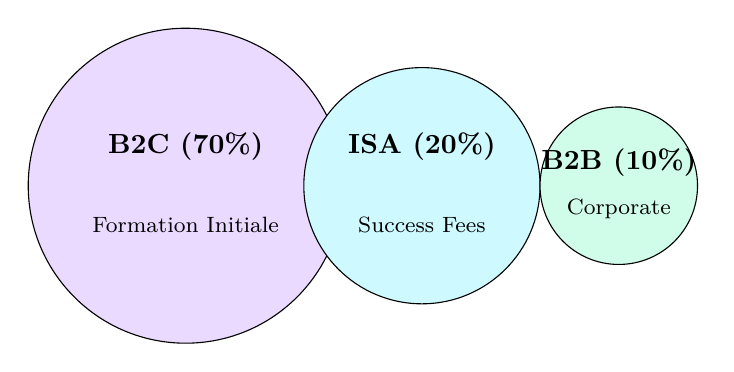
\begin{tikzpicture}
        \draw[fill=SolanaPurple!20] (0,0) circle (2cm);
        \node at (0,0.5) {\textbf{B2C (70\%)}};
        \node at (0,-0.5) {\footnotesize Formation Initiale};
        
        \draw[fill=SolanaBlue!20] (3,0) circle (1.5cm);
        \node at (3,0.5) {\textbf{ISA (20\%)}};
        \node at (3,-0.5) {\footnotesize Success Fees};
        
        \draw[fill=SolanaGreen!20] (5.5,0) circle (1cm);
        \node at (5.5,0.3) {\textbf{B2B (10\%)}};
        \node at (5.5,-0.3) {\footnotesize Corporate};
    \end{tikzpicture}
    \caption{Mix Revenus Cible (Année 3)}
\end{figure}

\section{Hypothèses & Sources du Modèle}

Ce modèle repose sur des données de marché comparables (Bootcamps Web3, Market Research 2024-2025).

\subsection{Hypothèses Clés}
\begin{itemize}
    \item \textbf{CAC (Coût d'Acquisition Client)} : Estimé à \textbf{250 TND / étudiant converti} (Campagnes LinkedIn/FB ciblées + SEO).
    \item \textbf{Salaire de Sortie Moyen} : Conservateur à \textbf{2 500 TND Net/Mois} (Marché local Senior) ou \textbf{1 500 \$} (Remote Junior Global).
    \item \textbf{Taux de Chute (Churn)} : 15\% entre chaque niveau (filtrage de qualité).
    \item \textbf{Taux de Placement} : 80\% à 6 mois (standard industrie pour formations sélectives).
\end{itemize}

\subsection{Structure des Coûts Directs}
\begin{itemize}
    \item \textbf{Mentorat} : Ratio 1:10. Rémunération horaire ou forfaitaire (Variable).
    \item \textbf{Infra} : Coût fixe LMS + Cloud (AWS/RPC) = 5\% du CA.
    \item \textbf{Légal/Admin} : 5\% du CA.
\end{itemize}

\section{Funnel d'Acquisition & Sourcing}

Le modèle de rentabilité dépend de la sélectivité en entrée (qualité des profils = placement garanti).

\begin{enumerate}
    \item \textbf{Top of Funnel (Leads)} : 1000 Inscrits Webinaire / Downloads Livre Blanc.
    \item \textbf{Middle of Funnel (Applicants)} : 200 Candidats passent le test technique Python/JS.
    \item \textbf{Bottom of Funnel (Selection)} : 50 Admissibles après entretien.
    \item \textbf{Conversion (Cohorte)} : 30 Inscrits payants (ou boursiers validés).
\end{enumerate}

Le ratio cible est de \textbf{3\% de conversion Lead $\to$ Client}, assurant une densité de talents élevée.

\section{Le Pilier B2B : Corporate Upskilling}

Pour réduire la dépendance aux frais de scolarité individuels, nous lançons une offre dédiée aux entreprises (Banques, ESN, Telcos) souhaitant monter une "Blockchain Factory" interne.

\textbf{Offre "Corporate Cohort" :}
\begin{itemize}
    \item \textbf{Principe :} Une entreprise réserve un bloc de 3 à 5 sièges dans une cohorte pour ses employés.
    \item \textbf{Tarif :} \textbf{15 900 TND / siège} (Premium Pricing).
    \item \textbf{Avantages :} Suivi RH dédié, Capstone orienté sur un Use-Case de l'entreprise, Clause de confidentialité.
    \item \textbf{Objectif :} 30\% du CA total en Année 3.
\end{itemize}

\section{Trajectoire Financière (36 Mois)}

La trésorerie est le nerf de la guerre. Notre modèle prend en compte le "Cash Drag" (décalage) des ISA.

\textbf{Projection du Volume Étudiant (Funnel) :}
\begin{center}
\small
\begin{tabular}{|l|c|c|c|}
\hline
\textbf{Niveau} & \textbf{Année 1} & \textbf{Année 2} & \textbf{Année 3} \\ \hline
\textbf{Niveau 1} (Foundations) & 30 & 60 & 90 \\ \hline
\textbf{Niveau 2} (Builder) & 20 & 40 & 60 \\ \hline
\textbf{Niveau 3} (Pro/Audit) & 12 & 24 & 36 \\ \hline
\end{tabular}
\end{center}

\begin{table}[H]
    \caption{Compte de Résultat et Trésorerie Prévisionnelle (TND)}
    \centering
    \small
    \rowcolors{2}{gray!5}{white}
    \begin{tabularx}{\textwidth}{|l|r|r|r|}
        \hline
        \textbf{Indicateur} & \textbf{Année 1 (Amorçage)} & \textbf{Année 2 (Scale)} & \textbf{Année 3 (Maturité)} \\ \hline
        \textbf{CA FORMATION (L1+L2+L3)} & \textbf{311 800} & \textbf{623 600} & \textbf{935 400} \\ \hline
        \textbf{CA ISA (Différé)} & 0 & 120 000 & 350 000 \\ \hline
        \textbf{CA SERVICES (B2B)} & 20 000 & 80 000 & 200 000 \\ \hline
        \textbf{TOTAL REVENUS} & \textbf{331 800} & \textbf{823 600} & \textbf{1 485 400} \\ \hline
        \textbf{DÉPENSES (OPEX)} & \textbf{260 000} & \textbf{520 000} & \textbf{880 000} \\ \hline
        \textit{(dont Salaires Staff)} & \textit{150 000} & \textit{300 000} & \textit{500 000} \\ \hline
        \textit{(dont Mentors Variable)} & \textit{60 000} & \textit{120 000} & \textit{200 000} \\ \hline
        \textbf{EBITDA} & \textbf{+71 800} & \textbf{+303 600} & \textbf{+605 400} \\ \hline
        \textit{Marge \%} & \textit{21\%} & \textit{37\%} & \textit{41\%} \\ \hline
    \end{tabularx}
\end{table}

\textbf{Analyse de Trésorerie :}
L'Année 1 est financée par le mix Upfront. L'effet de levier ISA commence à impacter significativement la trésorerie au milieu de l'Année 2, créant un "Fond de Roulement" naturel pour l'expansion.

\section{Analyse de Sensibilité}

Nous stress-testons le modèle selon 3 variables critiques.

\begin{table}[H]
    \caption{Sensibilité de l'EBITDA Année 2 (Objectif Cible 303k)}
    \centering
    \small
    \begin{tabular}{|l|c|c|l|}
        \hline
        \textbf{Variable} & \textbf{Variation} & \textbf{Impact EBITDA} & \textbf{Commentaire} \\ \hline
        Taux Placement & -20 pts & -50k & Impact différé sur ISA. \\ \hline
        Prix Bundle & -20\% & -120k & \textbf{Critique}. Nécessite réduction coûts Mentors. \\ \hline
        Conv. N1$\to$N2 & -15 pts & -90k & Critique. Nécessite meilleur sourcing S0. \\ \hline
    \end{tabular}
\end{table}

\subsection{Gestion du Risque Crédit ISA}
L'ISA est un actif financier qui comporte des risques spécifiques.
\begin{enumerate}
    \item \textbf{Recouvrement :} Nous intégrons une hypothèse de "Défaut Technique" de 15\% (étudiants ne payant pas malgré un emploi).
    \item \textbf{Mitigation :}
    \begin{itemize}
        \item \textbf{Juridique :} Contrat enregistré avec reconnaissance de dette.
        \item \textbf{Reputation :} Le SBT (Diplôme) est révocable ou marqué "En défaut" on-chain en cas d'impayé avéré, bloquant l'accès au réseau Alumni.
        \item \textbf{Incitations :} Bonus de fin de contrat si paiement anticipé.
    \end{itemize}
\end{enumerate}

\section{Financements et Partenariats Stratégiques}

Pour accélérer sans diluer le capital, RBK active les leviers non-dilutifs :

\subsection{1. Écosystème Web3 (Grants)}
\begin{itemize}
    \item \textbf{Solana Foundation :} Demande de grant "Education" pour financer les serveurs et les bourses (Target: 50k\$).
    \item \textbf{Superteam :} Sponsoring des Hackathons de fin de cohorte (Prize pool).
\end{itemize}

\subsection{2. Bailleurs de Fonds Institutionnels}
\begin{itemize}
    \item \textbf{Union Européenne (Erasmus+ / Horizon Europe) :} Projets de mobilité des talents numériques Afrique-Europe.
    \item \textbf{Banque Africaine de Développement (BAD) :} Programme "Coding for Jobs".
\end{itemize}

\subsection{3. Modèle de Franchise (Scale Africa)}
Dès l'Année 3, le modèle "RBK in a Box" (LMS + Programme + Brand) sera proposé en franchise à des hubs technologiques au Sénégal et en Côte d'Ivoire.
\begin{itemize}
    \item \textbf{Modèle :} Revenue Share (20\% du CA Franchise).
    \item \textbf{Apport :} RBK fournit la plateforme et la certification SBT. Le partenaire gère le local et le sourcing.
\end{itemize}


% 9. Marketing
\chapter{STRATÉGIE MARKETING \& ACQUISITION RENFORCÉE}

\section{Programme "Building in Public"}

RBK 2.0 ne fait pas de publicité, elle produit de la preuve. Notre stratégie d'acquisition repose sur le "Building in Public". Nous documentons publiquement nos succès, nos échecs, nos audits et nos outils.
Cette transparence radicale a trois objectifs :
1. \textbf{Crédibilité :} Montrer le niveau technique réel avant même l'inscription.
2. \textbf{Confiance :} Rassurer les candidats (et leurs parents) sur le sérieux de la pédagogie.
3. \textbf{Communauté :} Attirer des mentors et des entreprises qui partagent nos valeurs.

\paragraph{Les 3 Piliers de Contenu}
\begin{enumerate}
    \item \textbf{Technique (The Code) :} Partage de snippets Rust, analyses de hacks récents, tutoriels Solana. Cible : Développeurs, CTOs.
    \item \textbf{Pédagogie (The Journey) :} Avant/Après des étudiants, rediffusion de Code Reviews, partage de ressources (Cheat Sheets). Cible : Candidats.
    \item \textbf{Success Stories (The Result) :} Interviews d'Alumni, montants des bounties gagnés, projets lancés. Cible : Grand public.
\end{enumerate}

\begin{figure}[H]
    \centering
    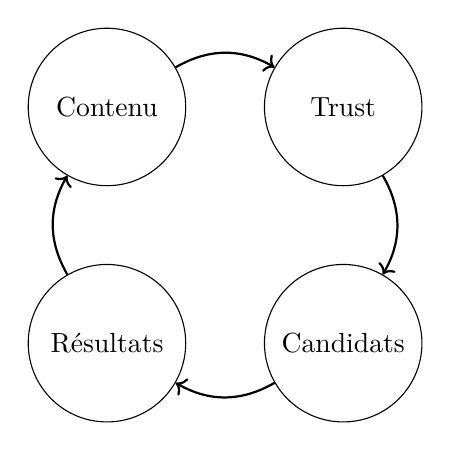
\begin{tikzpicture}
        \node[circle, draw, minimum size=2cm] (content) {Contenu};
        \node[circle, draw, minimum size=2cm, right of=content, node distance=3cm] (community) {Trust};
        \node[circle, draw, minimum size=2cm, below of=community, node distance=3cm] (apply) {Candidats};
        \node[circle, draw, minimum size=2cm, left of=apply, node distance=3cm] (result) {Résultats};
        
        \draw[->, thick, bend left] (content) to (community);
        \draw[->, thick, bend left] (community) to (apply);
        \draw[->, thick, bend left] (apply) to (result);
        \draw[->, thick, bend left] (result) to (content);
    \end{tikzpicture}
    \caption{Flywheel Building in Public}
\end{figure}

\begin{table}[H]
    \caption{Calendrier Éditorial Type (Cycle 12 Semaines)}
    \centering
    \small
    \rowcolors{2}{gray!10}{white}
    \begin{tabularx}{\textwidth}{|l|l|l|X|}
        \hline
        \textbf{Semaine} & \textbf{Thème} & \textbf{Canal} & \textbf{KPI Cible} \\ \hline
        S1-S4 & Rust Tips \& Tricks & Twitter/X & 10k Impressions \\ \hline
        S5-S8 & Démo Projets Élèves & YouTube/LinkedIn & 50 Leads (Inscrits Webinar) \\ \hline
        S9-S12 & Audit \& Sécurité & Blog/Medium & 5 Partenariats Entreprise \\ \hline
    \end{tabularx}
\end{table}

\section{Simulateur de ROI Interactif}

Pour contrer l'objection du prix, nous proposons un outil permettant de comparer 3 scénarios d'investissement. L'objectif est de montrer que le risque est nul si on commence petit.

\paragraph{Les 3 Options du Simulateur}
\begin{enumerate}
    \item \textbf{Option A (Prudent) :} Niveau 1 seul (2 900 TND). Objectif : Tester son appétence. Risque minime.
    \item \textbf{Option B (Standard) :} Niveau 1 + Upgrade Bundle. Coût total $\approx$ 14 900 TND. Objectif : Flexibilité.
    \item \textbf{Option C (Engagé) :} Bundle Upfront (14 900 TND). Objectif : Économie maximale immédiate.
\end{enumerate}

\begin{center}
\fbox{\begin{minipage}{0.9\textwidth}
\textbf{Exemple Chiffré : Le "Smart Start"} \\
\textit{Profil :} Étudiant, hésitant. \\
\textit{Action :} S'inscrit au \textbf{Niveau 1} (2 900 TND). \\
\textit{Résultat :} Valide ses acquis en 8 semaines. Réalise un premier Bounty de 500\$. \\
\textit{Décision :} Réinvestit le bounty dans l'upgrade Bundle. \\
\textbf{ROI :} Il a financé 50\% de son N1 par le code avant même de finir.
\end{minipage}}
\end{center}

\begin{table}[H]
    \caption{ROI Comparatif par Option (Sortie Junior : 3 000 TND/mois)}
    \centering
    \small
    \rowcolors{2}{gray!5}{white}
    \begin{tabularx}{\textwidth}{|l|l|l|X|}
        \hline
        \textbf{Option} & \textbf{Coût Total} & \textbf{Délai ROI} & \textbf{Avantage} \\ \hline
        N1 Seul & 2 900 TND & 1 mois & Test Low-cost \\ \hline
        Bundle & 14 900 TND & 5 mois & Accès complet + Job \\ \hline
        ISA & 15\% Salaire & Dès 1er salaire & Pas de cash upfront \\ \hline
    \end{tabularx}
\end{table}

\section{Stratégie Multi-Canaux}

Nous ne cherchons pas à être partout, mais à dominer 5 canaux spécifiques où se trouve notre cible "Elite".

\paragraph{Les 5 Canaux Prioritaires}
\begin{enumerate}
    \item \textbf{LinkedIn (La Vitrine) :} Pour les parents, les recruteurs et les partenariats corporatifs. \textit{Cadence : 2 posts/semaine.}
    \item \textbf{X / Twitter (L'Arène) :} Pour la crédibilité technique crypto, les news Rust, et l'engagement communautaire. \textit{Cadence : Quotidien.}
    \item \textbf{YouTube (La Preuve) :} Replays de workshops, Démos de Capstones, Témoignages. \textit{Cadence : 2 vidéos/mois.}
    \item \textbf{GitHub (Le CV) :} C'est notre canal d'acquisition "silencieux". Des repos propres et étoilés attirent les curieux techniques.
    \item \textbf{Discord (Le Salon) :} Conversion des leads chauds, support, Q\&A avant inscription.
\end{enumerate}

\begin{figure}[H]
    \centering
    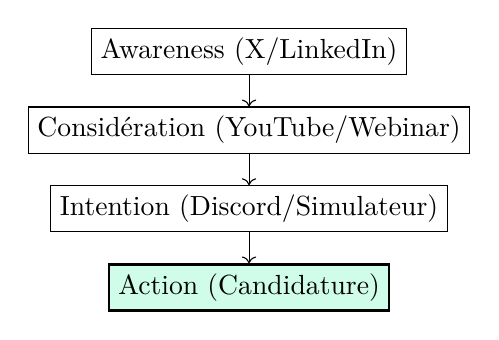
\begin{tikzpicture}
        \node[draw] (aware) {Awareness (X/LinkedIn)};
        \node[draw, below of=aware] (consider) {Considération (YouTube/Webinar)};
        \node[draw, below of=consider] (intent) {Intention (Discord/Simulateur)};
        \node[draw, below of=intent, thick, fill=SolanaGreen!20] (action) {Action (Candidature)};
        
        \draw[->] (aware) -- (consider);
        \draw[->] (consider) -- (intent);
        \draw[->] (intent) -- (action);
    \end{tikzpicture}
    \caption{Funnel d'Acquisition Simplifié}
\end{figure}

\section{Programme de Référence \& Bounties}

Le "Word of Mouth" est notre canal le plus rentable (CAC $\approx$ 0). Nous l'industrialisons.

\paragraph{Système de Parrainage (Referral)}
Tout Alumni ou Étudiant validé peut parrainer un candidat.
\begin{itemize}
    \item \textbf{Pour le Parrain :} 500 TND (Cash ou déduction ISA) versés APRÈS la validation de la Période d'Essai du filleul (Anti-fraude).
    \item \textbf{Pour le Filleul :} 5\% de réduction immédiate sur les frais Upfront.
\end{itemize}

\paragraph{Programme "Bug Bounties" Pédagogiques}
Nous payons (en crédits ou token réputation) pour l'amélioration du cursus.
\begin{itemize}
    \item Typo majeure dans le cours : 10 pts.
    \item Optimisation d'un exercice de code : 50 pts.
    \item Fix de sécurité sur l'infra école : 500 TND.
\end{itemize}
Cela crée une culture de "Contribution" dès le premier jour.

\begin{table}[H]
    \caption{Catalogue des Incentives}
    \centering
    \small
    \begin{tabularx}{\textwidth}{|l|l|l|X|}
        \hline
        \textbf{Mécanisme} & \textbf{Bénéficiaire} & \textbf{Récompense} & \textbf{Condition Anti-Fraude} \\ \hline
        Parrainage & Alumni & 500 TND & Filleul valide le SPRINT 1 (pas juste inscrit). \\ \hline
        Ambassadeur & Influenceur & 10\% Commission & Lien tracké + KYC obligatoire. \\ \hline
        Bounty Code & Étudiant & Goodies / Cash & Pull Request validée par le Lead Tech. \\ \hline
    \end{tabularx}
\end{table}


% 10. Analyse des Risques
\chapter[⚠️ ANALYSE DES RISQUES \& MODÈLE DE RÉSILIENCE]{ANALYSE DES RISQUES \& MODÈLE DE RÉSILIENCE}
\label{chap:risques}

RBK 2.0 opère à l'intersection de deux secteurs volatils : l'éducation technologique et les actifs numériques. Cette position exige une gestion des risques de niveau institutionnel.

\section{Risques Réglementaires et Conformité}

La pérennité de RBK repose sur une veille juridique proactive, particulièrement en Tunisie (siège opérationnel) et en Europe (marché cible).

\subsection{Loi des Changes et Crypto-Actifs (Tunisie)}
\textbf{Risque :} La détention de crypto-actifs reste une zone grise. Une interdiction stricte pourrait bloquer les paiements en Stablecoins.
\textbf{Mitigation :}
\begin{itemize}
    \item \textbf{Structure Off-shore :} RBK facture via une entité non-résidente (ou partenaire) pour les flux internationaux, en conformité totale avec le code des changes.
    \item \textbf{Flux Fiat Prioritaire :} 100\% des frais de scolarité locaux sont encaissés en TND via virement bancaire classique. La crypto n'est qu'un rail technologique optionnel pour les bourses étrangères.
    \item \textbf{Lobbying Actif :} RBK participe aux groupes de travail de la BCT (Banque Centrale) pour encadrer le statut de "Service Exporter" blockchain.
\end{itemize}

\subsection{GDPR et Données Étudiantes On-Chain}
\textbf{Risque :} Les SBT (Soulbound Tokens) sont immuables. Si des données personnelles y sont inscrites, le "Droit à l'oubli" est impossible.
\textbf{Mitigation :}
\begin{itemize}
    \item \textbf{Architecture Privacy-First :} Aucun nom, email ou IP n'est stocké sur la blockchain. Le SBT contient uniquement un \textit{Hash Cryptographique} (ex: `Keccak256(Diplome_PDF)`).
    \item \textbf{Consentement Explicite :} L'étudiant signe une décharge explicite pour le minting de ses résultats.
    \item \textbf{Droit à la Révocation :} Le contrat intelligent permet à l'admin (sur demande de l'étudiant) de "brûler" un token, rompant le lien public.
\end{itemize}

\subsection{Cadre Légal des ISA (Income Share Agreements)}
\textbf{Risque :} Requalification du contrat ISA en crédit à la consommation déguisé ou clause abusive.
\textbf{Mitigation :}
\begin{itemize}
    \item \textbf{Juridiction Compétente :} Contrats régis par le droit commercial (prestation de service avec paiement différé) et non le droit de la consommation.
    \item \textbf{Clauses Protectrices :} Plafond de remboursement (Cap) strict et durée limitée pour éviter toute notion de "servitude".
    \item \textbf{Enforceability :} Partenariat avec des cabinets de recouvrement locaux en Tunisie, Maroc et Côte d'Ivoire.
\end{itemize}

\section{Matrice de Risques Dynamique}

Nous évaluons la résilience du modèle selon trois scénarios de marché.

\begin{table}[h]
    \caption{Impact des Scénarios sur la Stratégie}
    \centering
    \footnotesize
    \rowcolors{2}{gray!5}{white}
    \begin{tabularx}{\textwidth}{|l|X|X|}
        \hline
        \textbf{Scénario} & \textbf{Contexte} & \textbf{Réponse Stratégique RBK} \\ \hline
        \textbf{Pessimiste} & "Crypto Winter" prolongé (-80\% Assets), Gel des embauches Web3. & Pivot vers formation \textbf{Rust Systems} (Automobile, Embarqué, Cloud). Réduction OPEX -40\%. Focus B2B (Upskilling). \\ \hline
        \textbf{Réaliste} & Croissance modérée (+15\%), Régulation stable, N1 $\to$ N2 conversion 50\%. & Exécution du plan standard. Mix ISA/Upfront 30/70. Ouverture d'un 2\textsuperscript{ème} track (EVM). \\ \hline
        \textbf{Optimiste} & "Bull Run" (+200\%), Pénurie critique de devs, Régulation favorable. & Accélération : Lancement Franchise Africa. Augmentation quota ISA à 50\% (trésorerie abondante). \\ \hline
    \end{tabularx}
\end{table}

\section{Plan de Réponse aux Incidents Crypto ("Black Swan")}

Face à la volatilité intrinsèque du secteur, nous déployons un plan de continuité "Grade Militaire".

\subsection{Scénario A : Effondrement de l'Écosystème Solana}
\textit{Déclencheur : Panne du réseau > 72 h ou chute du token SOL < 10\$.}
\begin{enumerate}
    \item \textbf{Immédiat (H+1) :} Communication de crise rassurance ("Nous formons des ingénieurs, pas des spéculateurs").
    \item \textbf{Pivot Pédagogique (H+24) :} Bascule des modules "Solana Specific" vers "Rust Générique" (valable pour Polkadot, Near, ou Backend Web2).
    \item \textbf{Trésorerie :} Conversion automatique de tous les assets crypto en Fiat/Stablecoin dès que la volatilité dépasse un seuil d'alerte (Stop-Loss).
\end{enumerate}

\subsection{Scénario B : Hack d'un Bridge / Protocole Partenaire}
\textit{Déclencheur : Un outil utilisé dans le cours (ex: Wormhole) est compromis.}
\begin{enumerate}
    \item \textbf{Arrêt des Nodes :} Les étudiants déconnectent leurs environnements de dev locaux.
    \item \textbf{Learning Moment :} L'incident devient un cas d'étude "Live". Analyse on-chain du hack en cours de sécurité.
    \item \textbf{Fonds de Sécurité :} Si des bourses étudiantes étaient bloquées, le Fonds de Garantie RBK avance la liquidité.
\end{enumerate}

\section{Tableau de Bord des Risques Critiques}

\begin{table}[h]
    \caption{Top 5 Risques et Mitigations (2026)}
    \centering
    \small
    \begin{tabularx}{\textwidth}{|l|c|c|X|}
        \hline
        \textbf{Risque} & \textbf{Prob.} & \textbf{Imp.} & \textbf{Plan de Mitigation} \\ \hline
        Défaut Paiement ISA & 3/5 & 5/5 & Sélection stricte (Top 30\%), Fonds de Garantie (120k TND), Assurance. \\ \hline
        Obsolescence Tech & 4/5 & 3/5 & Comité Pédagogique trimestriel, Track Agnostique (Focus Fundamentals). \\ \hline
        Fuite des Mentors & 2/5 & 4/5 & Programme "Train the Trainer", Satisfaction Index, Bonus Performance. \\ \hline
        Cyber-attaque École & 3/5 & 4/5 & Infra isolée, 2FA Hardware (Yubikey) pour staff, Audit annuel. \\ \hline
        Perte Réputation & 2/5 & 5/5 & Transparence totale (Building in Public), Charte Éthique stricte. \\ \hline
    \end{tabularx}
\end{table}


% 15. Compliance (NOUVEAU)
\chapter{COMPLIANCE \& RÉGULATION WEB3 – GUIDE PRATIQUE}
\label{chap:compliance}

Ce chapitre transforme la contrainte réglementaire en avantage compétitif. Dans le Web3, la conformité n'est pas un frein, mais une fonctionnalité architecturale.

\section{KYC/AML Décentralisé – La Conformité par la Technologie}

\subsection{Philosophie du "Privacy by Design"}
Nous enseignons à passer du KYC centralisé (documents stockés sur serveur vulnérable) à l'\textbf{Identité Auto-Souveraine (SSI)} et aux **Preuves à Divulgation Nulle de Connaissance (ZK-Proofs)}.

\subsection{Architecture Technique}
\begin{enumerate}
    \item \textbf{Vérification (Claim)} : L'utilisateur se vérifie une fois auprès d'un Issuer (ex: Civic) et reçoit une "Verifiable Credential" (VC).
    \item \textbf{Stockage (Wallet)} : La VC est stockée localement dans le portefeuille de l'utilisateur.
    \item \textbf{Preuve (Proof)} : Pour accéder à un protocole, le portefeuille génère une preuve ZK : "J'ai +18 ans et je ne suis pas résident US", \textbf{sans révéler l'identité réelle}.
\end{enumerate}

\subsection{Stack Pratique Enseignée}
\begin{itemize}
    \item \textbf{Polygon ID} : Création de contrats de staking avec gating géographique via VC.
    \item \textbf{Civic Pass} : Protection anti-sybil pour les airdrops.
    \item \textbf{Sismo} : Badges ZK pour la réputation (gouvernance DAO).
\end{itemize}

\section{GDPR \& Données On-Chain}

\subsection{Le Conflit Immuabilité vs Droit à l'Oubli}
Règle d'or : \textbf{Jamais de PII (Personally Identifiable Information) on-chain}.

\subsection{Patterns Architecturaux}
\begin{itemize}
    \item \textbf{Hash-Only} : Stocker `keccak256(data)` on-chain. La donnée réelle est off-chain avec contrôle d'accès.
    \item \textbf{Chiffrement Asymétrique} : Données chiffrées avec la clé publique du destinataire.
    \item \textbf{Pointeurs IPFS} : Stocker uniquement le CID (Content ID) sur la blockchain.
\end{itemize}

\section{Fiscalité Crypto \& Statut ETE}

\subsection{Le Guide de l'Ingénieur-Exportateur}
Les revenus en crypto sont des revenus en devises étrangères. Le statut ETE (Entreprise Totalement Exportatrice) est la clé de l'optimisation légale.

\subsection{Flux Financier Recommandé}
\begin{enumerate}
    \item \textbf{Réception} : Client $\to$ Passerelle (Grey.co/Bitwage) $\to$ Virement TND.
    \item \textbf{Comptabilité} : Enregistrement au taux du jour BCT.
    \item \textbf{Déclaration} : Trimestrielle auprès de la banque centrale.
\end{enumerate}


% 11. Roadmap
\input{chapters/15_roadmap.tex}

% 12. Token & Alumni
\chapter{TOKEN DE RÉPUTATION \& ALUMNI PROGRAM}

\section{RBK Soulbound Tokens (SBTs)}

Le diplôme papier est obsolète. RBK 2.0 certifie les compétences via des \textbf{Soulbound Tokens (SBTs)} : des jetons numériques non-transférables, infalsifiables, et vérifiables instantanément sur la blockchain.
Ce n'est pas un actif financier (pas de prix, pas de marché secondaire). C'est un \textbf{CV cryptographique}. Chaque SBT représente une compétence acquise ("Rust Ace"), une réalisation ("Capstone Winner") ou un rôle ("Mentor").

\paragraph{Architecture Technique \& Privacy}
Notre système respecte la confidentialité des étudiants.
\begin{itemize}
    \item \textbf{Issuer :} Un wallet Multisig (RBK Board) signe l'émission des badges.
    \item \textbf{Données :} Aucune donnée personnelle (Nom/Email) n'est stockée on-chain. Le SBT contient uniquement un Hash de la preuve (ex: hash du commit git ou du certificat PDF).
    \item \textbf{Vérification :} L'employeur utilise une dApp RBK pour vérifier la possession du badge et révéler le contenu associé si l'étudiant donne son accord (Signature).
\end{itemize}

\begin{figure}[h]
    \centering
    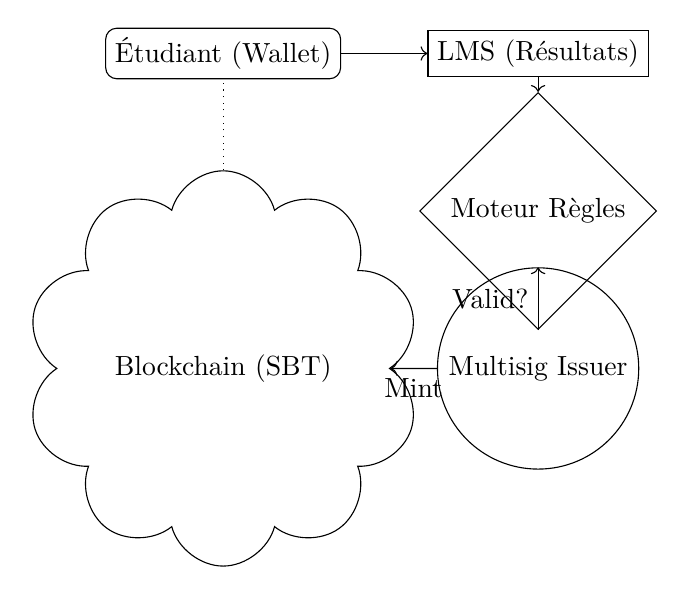
\begin{tikzpicture}[node distance=2cm, auto]
        \node[draw, rectangle, rounded corners] (student) {Étudiant (Wallet)};
        \node[draw, rectangle, right of=student, xshift=2cm] (lms) {LMS (Résultats)};
        \node[draw, diamond, below of=lms] (engine) {Moteur Règles};
        \node[draw, circle, below of=engine] (issuer) {Multisig Issuer};
        \node[draw, cloud, left of=issuer, xshift=-2cm] (chain) {Blockchain (SBT)};

        \draw[->] (student) -- (lms);
        \draw[->] (lms) -- (engine);
        \draw[->] (engine) -- node {Valid?} (issuer);
        \draw[->] (issuer) -- node {Mint} (chain);
        \draw[dotted] (chain) -- (student);
    \end{tikzpicture}
    \caption{Architecture d'Émission SBT}
\end{figure}

\begin{table}[h]
    \caption{Catalogue des Badges SBT (Extrait)}
    \centering
    \footnotesize
    \rowcolors{2}{gray!10}{white}
    \begin{tabularx}{\textwidth}{|l|l|X|l|}
        \hline
        \textbf{Badge} & \textbf{Niveau} & \textbf{Critères} & \textbf{Valeur Employeur} \\ \hline
        \textbf{RS-Elite} & Gold & Top 5\% Piscine Rust. & Capacité cognitive, résilience. \\ \hline
        \textbf{Solana-Arch} & Silver & Capstone validé avec Audit Clean. & "Production-Ready" Engineer. \\ \hline
        \textbf{Auditor-Jr} & Bronze & 3 Rapports de vulnérabilité soumis. & Conscience sécurité. \\ \hline
        \textbf{Team-Lead} & Silver & A géré une squad de 4 devs. & Soft skills, Management. \\ \hline
    \end{tabularx}
\end{table}

\begin{tcolorbox}[colback=SolanaBlue!5!white,colframe=SolanaBlue!75!black,title=Conformité \& Anti-Spéculation]
Les SBT RBK sont strictement incessibles. Si un wallet est compromis, le SBT est "brûlé" (revoked) et réémis vers une nouvelle adresse après vérification d'identité (KYC). Ils n'ont aucune valeur monétaire et ne donnent droit à aucun dividende.
\end{tcolorbox}

\section{Usages des SBT}

Les SBT ne sont pas des objets de collection, ce sont des clés d'accès ("Token Gating").

\paragraph{1. Vérification Employeur Instantanée}
Plus besoin d'appeler l'école pour vérifier un diplôme. L'employeur scanne l'adresse publique du candidat et voit instantanément ses certifications.

\begin{ceoBox}{Story : La Vérification en 3 secondes}
\textbf{Avant :} Un recruteur reçoit un PDF, doit appeler l'école, attendre 24h pour confirmer qu'il n'est pas falsifié. Coût : Temps + Risque.
\textbf{Avec RBK SBT :} Le recruteur colle l'adresse du candidat sur l'Explorer RBK. Le badge "Certified Graduate" apparaît instantanément avec la signature cryptographique de l'école et le lien vers le code du Capstone.
\textbf{Résultat :} Coût 0\$, 3 secondes, Confiance Absolue.
\end{ceoBox}

\paragraph{2. Accès au Job Board Premium}
Seuls les détenteurs du badge "Ready-to-Deploy" (cursus validé) peuvent voir les offres d'emploi exclusives de nos partenaires "Gold". Cela garantit aux recruteurs une qualité de candidature 100\% filtrée.

\paragraph{3. Gouvernance Alumni}
Le poids de vote dans la DAO Alumni est pondéré par les badges. Un "Senior Mentor" a plus de voix qu'un "New Grad" sur les décisions pédagogiques (mais pas financières).

\begin{table}[h]
    \caption{Usages et Bénéfices des SBT}
    \centering
    \small
    \begin{tabularx}{\textwidth}{|l|X|l|l|}
        \hline
        \textbf{Usage} & \textbf{Bénéfice} & \textbf{SBT Requis} & \textbf{Mécanisme} \\ \hline
        Job Board & Accès offres VIP & Certified Dev & Token Gating (Web3 Auth) \\ \hline
        Mentoring & Droit de devenir Mentor & Senior + Pedago & Whitelist Manuelle \\ \hline
        Bounties & Accès missions audit & Auditor Level 1 & Accès GitHub Repo privé \\ \hline
        Events & Tickets conférence gratuits & Active Member & Airdrop Ticket NFT \\ \hline
    \end{tabularx}
\end{table}

\section{Alumni Program Structuré}

L'Alumni Program est notre "Moat". C'est un réseau structuré qui continue d'apporter de la valeur des années après la sortie.

\paragraph{Structure en Tiers (Niveaux)}
L'engagement est gamifié via des statuts qui offrent des avantages croissants.
\begin{itemize}
    \item \textbf{Tier Bronze (New Grad) :} Accès Discord Alumni, Job Board, Annuaire. \textit{Condition : Diplômé.}
    \item \textbf{Tier Argent (Contributor) :} Accès Bounties rémunérés, Invitations Events VIP. \textit{Condition : A parrainé 1 étudiant OU donné 10h de mentorat.}
    \item \textbf{Tier Or (Legend) :} Accès Fonds Ventures, Siège au Conseil Pédago. \textit{Condition : A recruté un Alumni OU créé une startup RBK.}
\end{itemize}

\paragraph{Gouvernance}
Le Conseil Alumni (5 membres élus pour 6 mois) gère le budget "Community" (financé par 1\% des revenus de l'école). Ils décident des apéros, des workshops invités et des partenariats.
Règle Anti-Sybil : Seuls les wallets avec un SBT "Certified" actif depuis > 3 mois peuvent voter.

\begin{figure}[h]
    \centering
    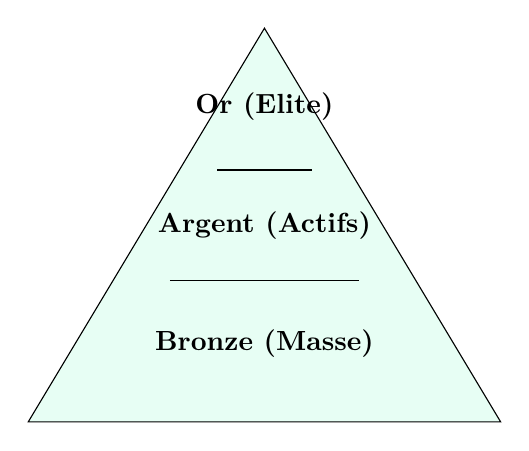
\begin{tikzpicture}
        \coordinate (A) at (0,0);
        \coordinate (B) at (6,0);
        \coordinate (C) at (3,5);
        \draw[fill=SolanaGreen!10] (A) -- (B) -- (C) -- cycle;
        \node at (3,1) {\textbf{Bronze (Masse)}};
        \node at (3,2.5) {\textbf{Argent (Actifs)}};
        \node at (3,4) {\textbf{Or (Elite)}};
        \draw (1.8, 1.8) -- (4.2, 1.8);
        \draw (2.4, 3.2) -- (3.6, 3.2);
    \end{tikzpicture}
    \caption{Pyramide des Tiers Alumni}
\end{figure}

\begin{table}[h]
    \caption{Roadmap Alumni (Année 1)}
    \centering
    \small
    \begin{tabularx}{\textwidth}{|l|l|X|l|}
        \hline
        \textbf{Trimestre} & \textbf{Initiative} & \textbf{KPI} & \textbf{Owner} \\ \hline
        Q1 & Lancement Discord & 100\% promo inscrite & Community Mgr \\ \hline
        Q2 & Premier Apéro Physique & 30 participants & Conseil Alumni \\ \hline
        Q3 & Programme Mentoring & 10 binômes actifs & Lead Pédago \\ \hline
        Q4 & Annuaire On-Chain & 100\% profils mintés & Tech Lead \\ \hline
    \end{tabularx}
\end{table}


% 13. Gouvernance & Éthique (NOUVEAU V4)
\chapter{GOUVERNANCE, ÉTHIQUE \& TRANSPARENCE}

RBK 2.0 aspire à devenir une institution de confiance. Cela exige une gouvernance partagée et une transparence radicale sur nos résultats.

\section{Comité Éthique \& Pédagogique (CEP)}

Le CEP est l'organe de contre-pouvoir indépendant qui garantit que l'école reste fidèle à sa mission.

\subsection{Composition (5 Membres)}
\begin{enumerate}
    \item \textbf{Président :} Une figure de la Tech en Tunisie (ex: CTO d'une Startup à succès, non lié à RBK).
    \item \textbf{Représentant Alumni :} Élu par la DAO des anciens.
    \item \textbf{Représentant Étudiants :} Délégué de la promo en cours.
    \item \textbf{Expert Éducation :} Un pédagogue ou universitaire.
    \item \textbf{Observateur Foundation :} Un membre de la Solana Foundation (Rôle consultatif).
    \item \textbf{CEO RBK :} Voix consultative (ne vote pas sur sa propre rémunération ou sa révocation).
\end{enumerate}

\subsection{Mandat}
Le CEP se réunit trimestriellement pour :
\begin{itemize}
    \item Valider les changements majeurs de curriculum.
    \item Arbitrer les contentieux ISA complexes (ex: demande de grâce pour cas de force majeure).
    \item Auditer les taux de placement déclarés.
\end{itemize}

\section{Transparence Radicale (Open Metrics)}

Contrairement aux écoles opaques, RBK publie ses KPI en temps réel sur une page publique "Status" (et on-chain).

\begin{techBox}{Metriques Publiques (Dashboard)}
    \begin{itemize}
        \item \textbf{Taux de Placement Réel :} Calculé à J+180 (CDI/Freelance).
        \item \textbf{Salaire Médian de Sortie :} Basé sur les fiches de paie anonymisées.
        \item \textbf{Taux de Remboursement ISA :} \% de recouvrement (indicateur de santé financière).
        \item \textbf{Diversité :} Ratio Homme/Femme et Répartition Géographique (Hors Grand Tunis).
    \end{itemize}
\end{techBox}

\section{Charte de Déontologie}

RBK s'engage formellement sur les points suivants :

\begin{enumerate}
    \item \textbf{Pas de Diplôme de Complaisance :} Un étudiant qui paie Upfront mais échoue aux examens techniques ne reçoit PAS de certification. Le niveau ne s'achète pas.
    \item \textbf{Consentement Éclairé ISA :} Chaque candidat reçoit une simulation "Worst Case" (Salaire élevé = Paiement max) avant de signer.
    \item \textbf{Neutralité Technologique :} Bien que financés par des écosystèmes (ex: Solana), nous enseignons l'ingénierie fondamentale, pas le dogmatisme. Nous critiquons les faiblesses de chaque chaine.
    \item \textbf{Protection des Données :} Refus de monétiser les données étudiants auprès de recruteurs tiers sans "Opt-in" spécifique.
\end{enumerate}

\section{Structure Juridique et Rôles (Branding)}

Pour assurer une clarté totale vis-à-vis des étudiants et partenaires, nous distinguons les entités comme suit :

\begin{description}
    \item[ReBootKamp (RBK) Tunisie :] L'entité légale opératrice historique. Elle porte l'agrément de formation, gère les locaux (Ariana), les contrats étudiants (ISA inclus via véhicule dédié) et le staff administratif. C'est le garant de la conformité locale.
    
    \item[Money Factory AI :] Le partenaire technologique et pédagogique exclusif. Basé à Dubai/Singapour, Money Factory fournit le curriculum "Cyborg", la plateforme LMS propriétaire, l'infrastructure de certification On-Chain (SBT) et l'accès au réseau international (Superteam, VCs).
    
    \item[Le Programme "RBK 2.0" :] Est le fruit de cette joint-venture : l'infrastructure opérationnelle de RBK propulsée par l'expertise technique de Money Factory AI.
\end{description}


% 14. Impact & ODD (NOUVEAU V4)
\chapter{IMPACT SOCIAL \& ALIGNEMENT ODD}

RBK 2.0 est une entreprise à mission. Notre but est de transférer de la richesse du PIB mondial (Web3) vers l'économie locale tunisienne et africaine.

\section{Contribution aux Objectifs de Développement Durable (ONU)}

\begin{itemize}
    \item \textbf{ODD 4 : Éducation de Qualité.} Nous démocratisons l'accès à une formation d'élite (niveau Ivy League) sans barrière financière grâce à l'ISA.
    \item \textbf{ODD 8 : Travail Décent et Croissance Économique.} Nous créons des emplois à haute valeur ajoutée, exportateurs de services, et rémunérés en devises fortes (via le statut local adéquat).
    \item \textbf{ODD 9 : Industrie, Innovation et Infrastructure.} Nous formons les architectes de l'infrastructure financière de demain.
\end{itemize}

\section{Indicateurs de Performance Sociale}

\subsection{1. Inclusion des Femmes dans la Tech}
Le Web3 souffre d'un déficit de diversité criant. RBK 2.0 met en place des mesures proactives :
\begin{itemize}
    \item \textbf{Bourses "Women in Web3" :} Le coût Upfront est réduit de 50\% pour les candidates validant la Piscine (financé par partenaires).
    \item \textbf{Objectif 2026 :} Atteindre 30\% de femmes par cohorte (vs 5\% moyenne secteur).
\end{itemize}

\subsection{2. Décentralisation Régionale}
Le talent est partout, les opportunités sont à la capitale.
\begin{itemize}
    \item \textbf{Recrutement National :} Roadshow dans les universités de l'intérieur (Sfax, Gabès, Gafsa).
    \item \textbf{Hébergement :} Partenariats avec des foyers pour faciliter l'installation à Tunis durant les 4 mois intensifs.
\end{itemize}

\subsection{3. Empreinte Carbone et Compensation}
La blockchain est perçue comme polluante. RBK nuance et agit :
\begin{itemize}
    \item \textbf{Choix Technologique :} Solana est une chaîne Proof-of-Stake dont une transaction consomme moins qu'une requête Google (0.0005 kWh).
    \item \textbf{Compensation :} Nous nous engageons à compenser 100\% de l'empreinte carbone de l'école (serveurs + clim + déplacements staff) via l'achat de crédits carbone certifiés on-chain (ex: Toucan Protocol).
\end{itemize}


% --- CHAPITRES COMPLEMENTAIRES ---
\chapter[Track A : Solana Engineer]{TRACK A : SOLANA SMART CONTRACT ENGINEER (RUST/ANCHOR)}

\section{Philosophie du Track : L'Excellence par Rust}

Solana n'est pas une simple blockchain rapide ; c'est un système d'exploitation décentralisé massivement parallèle (Sealevel). Pour y développer, comprendre la syntaxe ne suffit pas. Il faut maîtriser la gestion mémoire, la concurrence d'accès aux données (Account Model) et l'optimisation des cycles CPU (Compute Units).
Le choix de Rust n'est pas anodin : il impose une rigueur absolue (Safety) qui, combinée aux contraintes de Solana, forme des ingénieurs d'élite.
Notre objectif est de former des "Guardians" : des développeurs obsédés par la sécurité des fonds, la performance du code et la résilience de l'architecture.

\paragraph{Positionnement "Guardian"}
Un Guardian ne se contente pas de coder une feature. Il pense "adversarial". Il sait comment une transaction peut échouer, comment un attaquant peut manipuler une instruction, et comment le réseau va réagir sous charge. C'est un profil hybride entre Architecte Système et Auditeur de Sécurité.

\begin{tcolorbox}[colback=red!5!white,colframe=red!75!black,title=NON NÉGOCIABLE : LE STANDARD QUALITÉ]
	\begin{itemize}
		\item \textbf{Tests Systematiques :} Pas de PR sans tests (Unit + E2E). Coverage > 80\%.
		\item \textbf{Reproductibilité :} Builds déterministes (Verifiable Builds).
		\item \textbf{Audit-Readiness :} Code commenté, Documentation d'architecture jour 1, Threat Model explicite.
	\end{itemize}
\end{tcolorbox}

\begin{figure}[H]
	\centering
	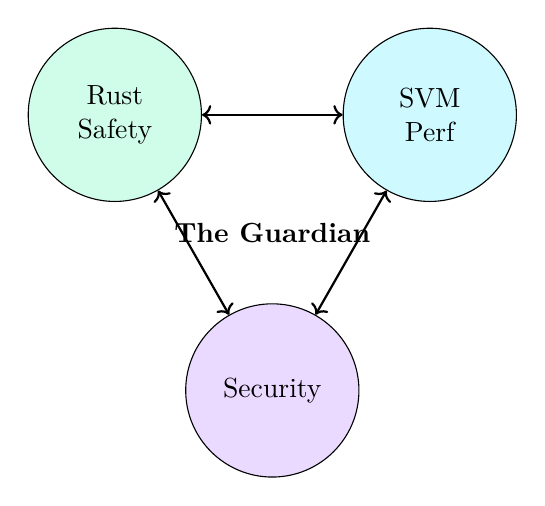
\begin{tikzpicture}
		\node[draw, circle, fill=SolanaGreen!20, minimum size=2.2cm, align=center] (rust) at (0,0) {Rust\\Safety};
		\node[draw, circle, fill=SolanaBlue!20, minimum size=2.2cm, align=center] (svm) at (4,0) {SVM\\Perf};
		\node[draw, circle, fill=SolanaPurple!20, minimum size=2.2cm, align=center] (secu) at (2,-3.5) {Security};
		\draw[<->, thick] (rust) -- (svm);
		\draw[<->, thick] (svm) -- (secu);
		\draw[<->, thick] (secu) -- (rust);
		\node[font=\bfseries] at (2, -1.5) {The Guardian};
	\end{tikzpicture}
	\caption{Pourquoi Solana est un track d'excellence}
	\label{fig:trackA_excellence}
\end{figure}

\begin{table}[H]
	\caption{Compétences Cibles vs Preuves}
	\centering
	\small
	\rowcolors{2}{gray!10}{white}
	\begin{tabularx}{\textwidth}{|l|X|X|l|}
		\hline
		\textbf{Domaine} & \textbf{Compétence} & \textbf{Preuve Attendue}        & \textbf{Standard} \\ \hline
		Architecture     & Gestion PDAs        & Diagramme de dérivations        & Pas de collision  \\ \hline
		Sécurité         & Signer Checks       & Tests d'invocation malveillante & 100\% checked     \\ \hline
		Performance      & CU Optimization     & Rapport profilage transaction   & < 200k CU         \\ \hline
	\end{tabularx}
\end{table}

\section{Structure Pédagogique : De l'Architecture au Produit (16 Semaines)}
Le cursus s'articule autour de la montée en puissance technique. (Voir le détail semaine par semaine dans le Syllabus Opérationnel en Annexe \ref{annexe:B3-syllabus48}).

Le parcours est découpé en 4 modules progressifs. On commence par "souffrir" avec Rust natif pour comprendre la mécanique interne, puis on accélère avec Anchor, avant de plonger dans l'architecture complexe (CPI) et le durcissement pour la production.
Chaque module se solde par un "Livrable Portfolio" qui prouve l'acquisition de la compétence.

\begin{tcolorbox}[colback=blue!5,colframe=blue!50,title=Syllabus Opérationnel]
	Le syllabus opérationnel détaillé est présenté dans l'\textbf{Annexe \ref{annexe:B3-syllabus48}}.
\end{tcolorbox}

\begin{table}[H]
	\caption{Carte des Modules (Résumé Exécutif)}
	\centering
	\small
	\begin{tabularx}{\textwidth}{|l|l|X|l|l|}
		\hline
		\textbf{Module} & \textbf{Sem} & \textbf{Objectif}          & \textbf{Lab Principal} & \textbf{Portfolio} \\ \hline
		1. Native       & 13-16        & Comprendre l'Account Model & Mini-Vault Natif       & Repo "Raw"         \\ \hline
		2. Anchor       & 17-20        & Productivité               & Marketplace NFT        & Program IDL        \\ \hline
		3. Arch         & 21-24        & Composabilité              & CPI Orchestrator       & Diagramme Arch     \\ \hline
		4. Prod         & 25-28        & Hardening                  & Full dApp              & Audit Report       \\ \hline
	\end{tabularx}
\end{table}

\subsection{MODULE 1 : Le Modèle Solana \& Rust Natif (Semaines 13-16)}

\paragraph{Objectifs Opérationnels}
\begin{itemize}
	\item Maîtriser la dé-sérialisation manuelle des données (Borsh).
	\item Gérer le "Rent" et l'allocation d'espace (realloc).
	\item Comprendre le cycle de vie d'une transaction (Signer, Writable).
\end{itemize}

\paragraph{Labs \& Livrables}
\textbf{Lab A (Messagerie \RBKTerm{onchain})} : Créer un programme qui permet à des utilisateurs de poster des messages stockés dans des comptes dédiés.
\textbf{Lab B (Mini-Escrow)} : Un contrat qui bloque des fonds jusqu'à validation par un tiers.
\textbf{Livrable :} Repo GitHub structuré avec tests TS (Mocha/Chai) interagissant avec `solana-test-validator`.

\begin{table}[H]
	\caption{Checklist Sécurité Module 1}
	\centering
	\footnotesize
	\begin{tabularx}{\textwidth}{|X|X|l|}
		\hline
		\textbf{Contrôle} & \textbf{Vérification}                                    & \textbf{Fail Typique} \\ \hline
		Owner Check       & Vérifier que \texttt{account\_info.owner == program\_id} & Injection de données  \\ \hline
		Signer Check      & Vérifier \texttt{account\_info.is\_signer}               & Usurpation            \\ \hline
		Rent Exempt       & Le compte est-il assez fondé ?                           & Compte purgé          \\ \hline
	\end{tabularx}
\end{table}

\subsection{MODULE 2 : Maîtrise du Framework Anchor (Semaines 17-20)}

\paragraph{Objectifs Opérationnels}
\begin{itemize}
	\item Utiliser les macros Anchor pour sécuriser le code (\texttt{\#[account(...)]}).
	\item Gérer les PDAs (Program Derived Addresses) de manière déterministe.
	\item Émettre des Events pour l'indexation.
\end{itemize}

\paragraph{Labs \& Livrables}
\textbf{Lab A (Counter PDA)} : Un compteur global et des compteurs user-specific utilisant des seeds.
\textbf{Lab B (Staking Vault)} : Un utilisateur dépose des tokens, le programme tracking le solde et le temps.
\textbf{Livrable :} Code Anchor propre, Tests TypeScript étendus, IDL publié.

\begin{figure}[H]
	\centering
	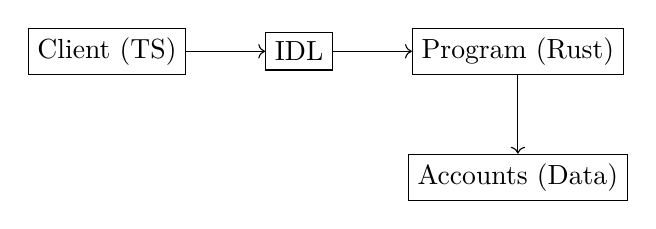
\begin{tikzpicture}
		\node[draw] (client) {Client (TS)};
		\node[draw, right=of client] (idl) {IDL};
		\node[draw, right=of idl] (prog) {Program (Rust)};
		\node[draw, below=of prog] (acc) {Accounts (Data)};
		\draw[->] (client) -- (idl);
		\draw[->] (idl) -- (prog);
		\draw[->] (prog) -- (acc);
	\end{tikzpicture}
	\caption{Flux Anchor}
\end{figure}

\subsection{MODULE 3 : Architectures Avancées \& Innovation (Semaines 21-24)}

\paragraph{Objectifs Opérationnels}
\begin{itemize}
	\item CPI (Cross-Program Invocations) : Appeler un programme depuis un autre (ex: Transfert SPL Token).
	\item Token Extensions (Token-2022) : Metadata, Transfer Hooks.
	\item Architecture Modulaire : Séparer la logique métier du stockage.
\end{itemize}

\paragraph{Labs \& Livrables}
\textbf{Lab A (CPI Challenge)} : Un programme "Master" qui contrôle un programme "Slave" via CPI signée (PDA Signer).
\textbf{Livrable :} Architecture complexe documentée (C4 Model) et tests d'intégration multi-programmes.

\subsection{MODULE 4 : Production Hardening \& UX Performance (Semaines 25-28)}

\paragraph{Objectifs Opérationnels}
\begin{itemize}
	\item Optimisation des Compute Units (CU) pour réduire les coûts et la latence.
	\item Gestion des erreurs custom et logs structurés.
	\item Préparation à l'audit (Freeze Authority, Upgradeability).
\end{itemize}

\paragraph{Projet Final}
Une dApp complète (ex: AMM simplifié ou DAO Voting) déployée sur Devnet, avec une UI fonctionnelle, une suite de tests \RBKTerm{ci_cd}, et un rapport d'auto-audit. La préparation inclut des contrôles \RBKTerm[Ops]{ops} pour sécuriser la mise en production.

\begin{table}[H]
	\caption{Production Readiness Review (PRR)}
	\centering
	\footnotesize
	\begin{tabularx}{\textwidth}{|l|l|X|l|}
		\hline
		\textbf{Domaine} & \textbf{Critère} & \textbf{Preuve}                 & \textbf{Statut} \\ \hline
		Sécurité         & Fuzzing Tests    & Corps de cas limites testés     & Obligatoire     \\ \hline
		Ops              & \RBKTerm{multisig} Upgrade & Clés gérées par Squads/\RBKTerm{multisig} & Obligatoire     \\ \hline
		Doc              & Architecture     & Diagramme Mermaid à jour        & Obligatoire     \\ \hline
	\end{tabularx}
\end{table}

\section{Stack Technique Spécifique}

La stack Solana évolue vite. Nous imposons une version LTS (Long Term Support) et des outils standards.

\begin{table}[H]
	\caption{Stack Track A (Standard)}
	\centering
	\small
	\begin{tabularx}{\textwidth}{|l|X|l|}
		\hline
		\textbf{Catégorie} & \textbf{Outils}                & \textbf{Usage}          \\ \hline
		Core               & Rust, Solana CLI, Anchor       & Dev, Deploy, Test       \\ \hline
		Client             & TypeScript, web3.js, Anchor.ts & Intégration Front/Tests \\ \hline
		Security           & Trident (Fuzzing), Soteria     & Audit auto              \\ \hline
		DevOps             & GitHub Actions, Solana Verify  & CI/CD                   \\ \hline
	\end{tabularx}
\end{table}

\section{Profil de Sortie : Le « Guardian »}

Le Guardian est un ingénieur rare. Il ne "bricole" pas des scripts. Il construit des infrastructures financières immuables. Il est capable de livrer un protocole \RBKTerm{defi} sécurisé, documenté et performant en autonomie.
Son employabilité est maximale car il maîtrise la chaîne de valeur complète : du bas niveau (Rust/BPF) au haut niveau (Architecture/Produit).

\paragraph{Missions Types en Entreprise}
\begin{itemize}
	\item Construire un DEX (Decentralized Exchange) à haute fréquence.
	\item Auditer un protocole de Lending pour détecter les failles de liquidité.
	\item Optimiser les coûts de gas d'un programme NFT à fort volume (Compression).
\end{itemize}

\begin{table}[H]
	\caption{Checklist Portfolio Guardian}
	\centering
	\small
	\begin{tabularx}{\textwidth}{|l|X|l|}
		\hline
		\textbf{Artefact} & \textbf{Contenu}                     & \textbf{Critère}      \\ \hline
		3 Repos GitHub    & Code Rust clean, Tests, CI           & Green CI Badge        \\ \hline
		Audit Report      & Analyse d'un protocole tiers         & 3 failles identifiées \\ \hline
		Demo Live         & Vidéo Loom (3 min) expliquant l'arch & Clarté orale          \\ \hline
	\end{tabularx}
\end{table}

\chapter[Track B : EVM Engineer]{TRACK B : EVM ENGINEER (SOLIDITY/FOUNDRY)}

\section{Philosophie du Track : La Maîtrise du Standard Industriel}

L'\RBKTerm{evm} (Ethereum Virtual Machine) est le standard mondial des smart contracts. Maîtriser Solidity et Foundry, c'est s'ouvrir les portes de l'écosystème le plus riche (Ethereum, Arbitrum, Optimism, Base, Polygon).
Notre approche est "Infrastructure-First". Nous ne formons pas des développeurs qui copient-collent du code OpenZeppelin, mais des ingénieurs capables de comprendre le stockage bas niveau, l'optimisation du Gas et les subtilités des upgrades (Proxies).

\paragraph{Positionnement "Infra Engineer"}
L'ingénieur \RBKTerm{evm} RBK est un bâtisseur de protocoles. Il maîtrise la chaîne DevOps (Foundry, \RBKTerm[CI]{ci_cd}, Verification), la sécurité offensive (Fuzzing, Invariants) et les patterns de composabilité (\RBKTerm{defi} Lego).

\begin{tcolorbox}[colback=blue!5!white,colframe=blue!75!black,title=NON NÉGOCIABLE : AUDIT-READINESS]
\begin{itemize}
    \item \textbf{Test-First :} TDD strict avec Foundry. Fuzzing obligatoire.
    \item \textbf{Gas Optimization :} Chaque Opcode compte (Assembly si nécessaire).
    \item \textbf{Security Mindset :} "Don't trust, verify". Protection Reentrancy, Overflow, Access Control.
\end{itemize}
\end{tcolorbox}

\begin{figure}[H]
    \centering
    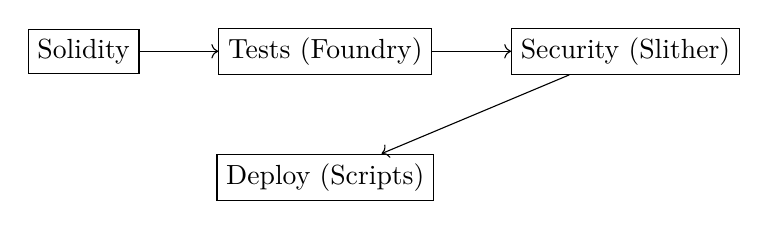
\begin{tikzpicture}
        \node[draw, rectangle] (sol) {Solidity};
        \node[draw, rectangle, right=of sol] (test) {Tests (Foundry)};
        \node[draw, rectangle, right=of test] (sec) {Security (Slither)};
        \node[draw, rectangle, below=of test] (deploy) {Deploy (Scripts)};
        \draw[->] (sol) -- (test);
        \draw[->] (test) -- (sec);
        \draw[->] (sec) -- (deploy);
    \end{tikzpicture}
    \caption{Chaîne de Valeur EVM}
    \label{fig:trackB_valuechain}
\end{figure}

\section{Structure Pédagogique : De la Logique au Durcissement (16 Semaines)}

Un parcours intensif qui commence par les fondations (Storage Layout) pour aller jusqu'au déploiement multi-chain complexe.

\begin{table}[H]
    \caption{Carte des Modules Track B}
    \centering
    \small
    \begin{tabularx}{\textwidth}{|l|l|X|l|}
        \hline
        \textbf{Module} & \textbf{Sem} & \textbf{Objectif} & \textbf{Livrable} \\ \hline
        1. Basics & 13-15 & EVM Internals & Vault Natif \\ \hline
        2. Pro Env & 16-18 & Foundry Mastery & CI Pipeline \\ \hline
        3. Standards & 19-21 & ERC20/721 & Token System \\ \hline
        4. dApp & 22-24 & Intégration & Full Stack dApp \\ \hline
        5. Scaling & 25-26 & L2 \& Upgrades & UUPS Proxy \\ \hline
        6. Hardening & 27-28 & Sécurité & Audit Report \\ \hline
    \end{tabularx}
\end{table}

\subsection{MODULE 1 : Smart Contract Basics \& Solidity Deep Dive (Semaines 13-15)}

\paragraph{Objectifs}
Comprendre comment l'EVM stocke les données (Slots), la différence Memory/CallData, et les structures de contrôle de base.
\textbf{Lab A (Vault Sécurisé)} : Un contrat de dépôt/retrait avec gestion des rôles (Ownable).
\textbf{Critères :} Tests de cas nominaux et d'erreurs (Revert).

\subsection{MODULE 2 : Environnement de Développement Pro (Semaines 16-18)}

\paragraph{Objectifs}
Passer de Remix à Foundry. Maîtriser `forge test`, `cast`, et le Fuzzing.
\textbf{Lab (Test Suite)} : Écrire une suite de tests exhaustive (Unit + Fuzz) pour un protocole existant (ex: Uniswap V2 Pair simplifié).
\textbf{Livrable :} Repo avec GitHub Actions qui lance les tests à chaque PR.

\subsection{MODULE 3 : Token Standards \& Composabilité (Semaines 19-21)}

\paragraph{Objectifs}
Implémenter ERC20, ERC721, ERC1155. Comprendre `approve`, `transferFrom` et les risques associés.
\textbf{Lab (\RBKTerm{defi} Lego)} : Un contrat qui "wrap" un token pour ajouter du rendement (\RBKTerm{staking}).
\textbf{Critères :} Interopérabilité vérifiée avec les standards.

\subsection{MODULE 4 : dApp Development \& Web3 Integration (Semaines 22-24)}

\paragraph{Objectifs}
Connecter un Front (React/Next) au contrat via Wagmi/Viem. Gérer le cycle de vie de la transaction (Pending, Confirmed, Failed).
\textbf{Lab (Mini-DEX UI)} : Interface pour swapper des tokens (simulation).
\textbf{Checklist :} Gestion des erreurs \RBKTerm{rpc}, Feedback utilisateur.

\subsection{MODULE 5 : L2 Scaling \& Advanced Patterns (Semaines 25-26)}

\paragraph{Objectifs}
Comprendre les Rollups (Optimistic/ZK). Déployer sur Arbitrum/Base. Gérer l'upgradeabilité (Proxies).
\textbf{Lab (UUPS Upgrade)} : Déployer une V1, puis upgrader vers une V2 sans perdre l'état (Storage).

\subsection{MODULE 6 : Production Hardening \& Security (Semaines 27-28)}

\paragraph{Objectifs}
Sécurisation finale. Audit interne.
\textbf{Projet Final :} Déploiement d'un protocole complet sur Testnet (Sepolia/Goerli) avec scripts de vérification Etherscan automatisés.

\begin{table}[H]
    \caption{Security Checklist EVM}
    \centering
    \small
    \begin{tabularx}{\textwidth}{|l|X|l|}
        \hline
        \textbf{Vulnérabilité} & \textbf{Contrôle} & \textbf{Outil} \\ \hline
        Reentrancy & Checks-Effects-Interactions & Slither \\ \hline
        Access Control & Modifiers corrects & Manual Review \\ \hline
        Arithmetic & Overflow (Solidity <0.8 checked) & Fuzzing \\ \hline
    \end{tabularx}
\end{table}

\section{Stack Technique Spécifique}

On privilégie la stack moderne (Rust-based) pour sa rapidité.

\begin{table}[H]
    \caption{Stack Track B (Foundry)}
    \centering
    \small
    \begin{tabularx}{\textwidth}{|l|X|l|}
        \hline
        \textbf{Catégorie} & \textbf{Outils} & \textbf{Usage} \\ \hline
        Framework & Foundry (Forge, Cast, Anvil) & Tout-en-un \\ \hline
        Libs & OpenZeppelin Contracts & Standards sécu \\ \hline
        Client & Viem, Wagmi & Front-end \\ \hline
        Analysis & Slither, Aderyn & Static Analysis \\ \hline
    \end{tabularx}
\end{table}

\section{Profil de Sortie : L'Ingénieur d'Infrastructure EVM}

L'Ingénieur EVM RBK est prêt pour intégrer une équipe Core Protocol ou une start-up \RBKTerm{defi}. Il sait écrire du code qui gère des millions de dollars.

\paragraph{Missions Types en Entreprise}
\begin{itemize}
    \item Développer une stratégie de Loop \RBKTerm{staking} sur un protocole de Lending (ex: Aave).
    \item Migrer un token Gouvernance d'un Layer 1 vers un Layer 2 (\RBKTerm{bridge} Architecture).
    \item Écrire les scripts de déploiement automatisés pour une collection NFT de 10k pièces avec whitelist Merkle Tree.
\end{itemize}

La trajectoire comprend un volet \RBKTerm[Ops]{ops} pour fiabiliser les déploiements et vérifier les contrats.

\begin{table}[H]
    \caption{Matrice Compétences Infra EVM}
    \centering
    \small
    \begin{tabularx}{\textwidth}{|l|X|l|}
        \hline
        \textbf{Domaine} & \textbf{Attendu} & \textbf{Preuve} \\ \hline
        Solidity & Expert (Storage, Assembly) & Gas Golfing Repo \\ \hline
        Testing & Expert (Fuzzing, Invariants) & Coverage > 95\% \\ \hline
        Ops & Autonome (Scripts, Verify) & Déploiements vérifiés \\ \hline
    \end{tabularx}
\end{table}

\chapter{TRACK C : PRODUCT \& GROWTH ENGINEER (FULL STACK + ANALYTICS)}

\section{Philosophie du Track : Le "Product Builder" Complet}

Le monde Web3 regorge de protocoles techniquement brillants mais inutilisables. Le Track C forme le chaînon manquant : l'ingénieur capable de construire une dApp de bout en bout (Front, Indexing, Analytics) et de piloter sa croissance.
Ce n'est pas un track "No-Code". C'est un track "Full-Code" orienté utilisateur. L'étudiant apprend à connecter les smart contracts au monde réel, à visualiser la data on-chain, et à itérer sur le produit en fonction des métriques.

\paragraph{Positionnement "Product Engineer"}
Il maîtrise la stack Next.js/React, l'indexation (Subgraphs/Squid), et l'analyse de données (Dune/SQL). Il sait que le code n'est qu'un moyen de livrer de la valeur.

\begin{tcolorbox}[colback=orange!5!white,colframe=orange!75!black,title=NON NÉGOCIABLE : USER-CENTRICITY]
\begin{itemize}
    \item \textbf{Zero-Friction :} Gérer les erreurs RPC, les wallets et l'UX dégradée sans perdre l'utilisateur.
    \item \textbf{Data-Driven :} Pas de feature sans tracking. Dashboard analytique jour 1.
    \item \textbf{Shipping :} Déploiement continu (Vercel/Fleek) et tests E2E (Playwright).
\end{itemize}
\end{tcolorbox}

\section{Structure Pédagogique : De l'UI à la Growth (12 Semaines)}

\begin{table}[h]
    \caption{Carte des Modules Track C}
    \centering
    \small
    \begin{tabularx}{\textwidth}{|l|l|X|l|}
        \hline
        \textbf{Module} & \textbf{Sem} & \textbf{Objectif} & \textbf{Livrable} \\ \hline
        1. Connectivity & 9-10 & Wallet & UI Integration & Multi-Wallet Connect \\ \hline
        2. Indexing & 11-12 & Data Availability & Custom Subgraph \\ \hline
        3. Analytics & 13-14 & SQL & On-chain Viz & Dune Dashboard \\ \hline
        4. Growth Eng & 15-16 & Viral Loops & Referral System \\ \hline
        5. Automation & 17-18 & Bots & Keepers & Telegram Bot \\ \hline
        6. Launch & 19-20 & Go-to-Market & Product Hunt Launch \\ \hline
    \end{tabularx}
\end{table}

\subsection{MODULE 1 : Web3 Connectivity \& State Management (Semaines 9-10)}

\paragraph{Objectifs}
Maîtriser la connexion Wallet (RainbowKit/Solana Adapter). Gérer l'état asynchrone (TanStack Query) et les erreurs RPC.
\textbf{Lab :} Créer un "Universal Profile Viewer" qui affiche les NFTs et soldes de n'importe quelle adresse (EVM+SVM).

\subsection{MODULE 2 : Indexing \& Data Layer (Semaines 11-12)}

\paragraph{Objectifs}
La blockchain est une mauvaise base de données de lecture. Apprendre à indexer les événements Smart Contract dans une DB relationnelle (Postgres) via The Graph ou Goldsky.
\textbf{Lab :} Indexer un DEX existant (ex: Uniswap) pour requêter les volumes par paire en < 100ms.

\subsection{MODULE 3 : On-Chain Analytics (Semaines 13-14)}

\paragraph{Objectifs}
SQL pour la blockchain. Utiliser Dune Analytics ou Flipside pour prouver la traction.
\textbf{Lab :} Créer un Dashboard "Whale Watcher" qui alerte sur les gros mouvements de stablecoins.

\subsection{MODULE 4 : Growth Engineering (Semaines 15-16)}

\paragraph{Objectifs}
Coder la viralité. Airdrops programmatiques, Whiteliists basées sur le comportement on-chain (Sybil resistance), Referral links on-chain.
\textbf{Lab :} Système de parrainage où le parrain reçoit une part des frais de transaction du filleul (Split par contrat).

\subsection{MODULE 5 : Automation & Bots (Semaines 17-18)}

\paragraph{Objectifs}
Interagir avec la blockchain sans interface web. Bots Telegram/Discord, Keepers (Chainlink Automation), Cron Jobs décentralisés.
\textbf{Lab :} Bot de sniping ou de notification de liquidation sur Aave.

\subsection{MODULE 6 : Production & Launch (Semaines 19-20)}

\paragraph{Objectifs}
Packaging final. Docs utilisateurs (GitBook), Landing page haute conversion, SEO Web3.
\textbf{Projet Final :} Une SaaS Web3 complet avec abonnement (Crypto-paiement) + Dashboard Admin.

\section{Profil de Sortie}

Un "Full Stack Web3" capable de lancer sa propre startup ou de rejoindre une équipe Growth dans un grand protocole.

\begin{table}[h]
    \caption{Matrice Compétences Product}
    \centering
    \small
    \begin{tabularx}{\textwidth}{|l|X|l|}
        \hline
        \textbf{Domaine} & \textbf{Attendu} & \textbf{Preuve} \\ \hline
        Front-end & Expert React/Next.js & App fluide 60fps \\ \hline
        Data & Capable d'écrire des subgraphs & API GraphQL \\ \hline
        Growth & Comprend les funnels & Analytics intégrés \\ \hline
    \end{tabularx}
\end{table}

\chapter{FICHES MÉTIERS \& ÉCONOMIE DU DIPLÔMÉ}

Ce chapitre détaille les 7 profils de sortie du cursus RBK. Chaque fiche est un standard industriel définissant les attentes, responsabilités et preuves exigées.

\section{Fiche Métier 1 : Smart Contract Engineer \& Auditor (Le « Guardian »)}

\paragraph{Résumé métier}
Le \textbf{Guardian} est le profil le plus critique : il construit des protocoles qui manipulent de la valeur et il sait les attaquer mentalement avant que d’autres ne le fassent. Il délivre du code \textbf{audit-ready}, documenté, testé, instrumenté, et il sait gérer le \textbf{post-prod} (incident, patch, gouvernance, communication).
Un Guardian qui ne sait pas écrire des tests négatifs et formaliser des invariants n’est pas “junior” : il est \textbf{dangereux}.

\paragraph{Mission et périmètre}
\begin{itemize}
    \item Concevoir et livrer des smart contracts (Solana/Anchor ou EVM selon track) avec \textbf{garanties} : invariants, contrôles d’accès, intégrité économique.
    \item Réaliser des audits internes et externes : revue “impitoyable”, modèle de menaces, classification des findings, correctifs, preuves.
    \item Organiser la \textbf{sécurité opérationnelle} : runbooks, multisig ops, war room, surveillance.
\end{itemize}

\paragraph{Responsabilités cœur (opérationnelles)}
\begin{enumerate}
    \item \textbf{Threat Modeling (avant le code)} : Définir actifs critiques, surfaces d’attaque, hypothèses. Produire un \textit{threat model} exploitable (STRIDE simplifié).
    \item \textbf{High-Assurance Coding} : Formaliser les invariants (soldes, monotonicité). Machine à états explicite.
    \item \textbf{Review \& Audit} : Revue structurée (checklist auth, CPI, oracles). Rédiger findings et findings.
    \item \textbf{Hardening (pré-prod)} : Tests négatifs, fuzz/invariants, quality gates bloquants.
    \item \textbf{Emergency Response} : War room, diagnostic, patch, rollback, communication.
\end{enumerate}

\paragraph{Trajectoire Carrière \& Mission}
\begin{itemize}
    \item \textbf{Junior (0-2 ans) :} Écrit des tests, corrige des bugs, audite des modules isolés. \textit{Mission : Implémenter le Staking Reward d'un protocole.}
    \item \textbf{Senior (3+ ans) :} Lead l'architecture, gère la War Room, valide les upgrades critiques. \textit{Mission : Sécuriser un Bridge cross-chain à 500M\$ TVL.}
\end{itemize}

\paragraph{Interactions}
Builder/PM (cadrage), dApp Engineer (API/erreurs), QA Engineer (stratégie tests), Visionnaire (hypothèses éco).

\paragraph{Livrables standard}
\texttt{docs/threat-model.md}, \texttt{AUDIT\_REPORT.md} (10 pages), Architecture doc, Tests suite (unit, int, fuzz), \texttt{RUNBOOK.md}.

\paragraph{KPIs}
Taux de findings critiques avant audit externe ("zéro surprise"), MTTR (correction vuln), Couverture utile, Fréquence incidents.

\begin{center}
    \textbf{Table: Matrice Compétence $\to$ Preuve $\to$ Outil} \\
    \small
    \begin{tabular}{|l|p{4.5cm}|l|}
        \hline
        \textbf{Compétence} & \textbf{Preuve attendue} & \textbf{Outil} \\ \hline
        Threat modeling & Threat model (actifs, surfaces) & STRIDE \\ \hline
        Sécurité & Tests négatifs auth/PDA/CPI & CI Checklist \\ \hline
        Audit mindset & Audit report protocole tiers & Markdown \\ \hline
        Fuzz / Invariants & Campagne fuzz + rapport & Trident/Foundry \\ \hline
        Hardening & Quality gates bloquants & CI/CD \\ \hline
        Perf budget & Profiling compute/gas & CLI / Gas report \\ \hline
        Post-prod ops & Runbook + war-room drill & Simulation \\ \hline
    \end{tabular}
\end{center}

\begin{figure}[h]
    \centering
    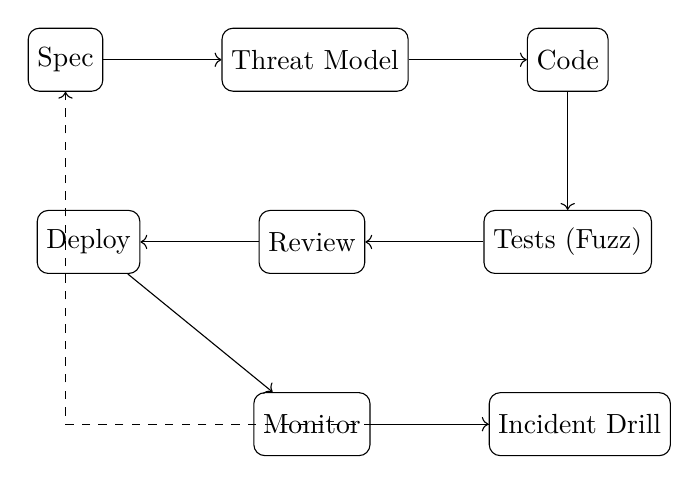
\begin{tikzpicture}[node distance=1.5cm, auto,
        block/.style={rectangle, draw, rounded corners, minimum height=0.8cm, text centered}]
        \node[block] (spec) {Spec};
        \node[block, right=of spec] (threat) {Threat Model};
        \node[block, right=of threat] (code) {Code};
        \node[block, below=of code] (test) {Tests (Fuzz)};
        \node[block, left=of test] (review) {Review};
        \node[block, left=of review] (deploy) {Deploy};
        \node[block, below=of review] (monitor) {Monitor};
        \node[block, right=of monitor] (incident) {Incident Drill};
        
        \draw[->] (spec) -- (threat);
        \draw[->] (threat) -- (code);
        \draw[->] (code) -- (test);
        \draw[->] (test) -- (review);
        \draw[->] (review) -- (deploy);
        \draw[->] (deploy) -- (monitor);
        \draw[->] (monitor) -- (incident);
        \draw[->, dashed] (incident) -| (spec);
    \end{tikzpicture}
    \caption{Boucle Guardian (SecDevOps)}
\end{figure}

\section{Fiche Métier 2 : Protocol \& Ecosystem Strategist (Le « Visionnaire »)}

\paragraph{Résumé métier}
Le Visionnaire transforme une idée en \textbf{système incitatif}. Il définit les règles économiques, le cadre de gouvernance et les risques. Il ne code pas le "comment", il rend le "quoi" mesurable.

\paragraph{Mission}
Concevoir tokenomics, governance (DAO), incentives. Produire simulations et plans de mitigation.

\paragraph{Responsabilités}
\begin{enumerate}
    \item \textbf{Tokenomics Design} : Émission, vesting, sinks/sources.
    \item \textbf{Incentive Modeling} : Boucles positives vs toxiques (Ponzi).
    \item \textbf{Governance} : Quorum, timelocks, emergency powers.
    \item \textbf{Risk Framing} : Depegging, bank-run, oracles.
    \item \textbf{Go-to-market} : Bounties, grants, amorçage.
\end{enumerate}

\begin{center}
    \textbf{Table: Livrables Visionnaire} \\
    \small
    \begin{tabular}{|l|p{5cm}|l|}
        \hline
        \textbf{Livrable} & \textbf{Contenu Minimum} & \textbf{Qualité} \\ \hline
        Litepaper & Vision, méca, roadmap & Clair, sans jargon \\ \hline
        Simulation Sheet & Modèle paramétrique & Rejouable \\ \hline
        Risk Register & Matrice Prob/Impact & Actionnable \\ \hline
        Governance Spec & Règles, quorum, rôles & Testable \\ \hline
        Incentive Plan & Rewards, budget, durée & Anti-mercenaire \\ \hline
    \end{tabular}
\end{center}

\section{Fiche Métier 3 : Web3 Product Builder / Entrepreneur (Le « Builder »)}

\paragraph{Résumé métier}
Le Builder est obsédé par la livraison. Il transforme un problème en produit utilisable. Il cadre le MVP, orchestre le delivery et garantit la qualité.

\paragraph{Responsabilités}
Product Discovery, Spec \& Scope, Delivery coordination, QA end-to-end, Business loop.

\begin{center}
    \textbf{Table: Definition of Done (Builder)} \\
    \small
    \begin{tabular}{|l|p{8cm}|}
        \hline
        \textbf{Axe} & \textbf{Critère DoD} \\ \hline
        Sécurité & Audit interne + Security Checklist + Bug Bounty \\ \hline
        Perf & TTF/Latence < seuil cible + Bench \\ \hline
        Obs & Dashboard actif (Retention, Churn, Erreurs) \\ \hline
        Docs & README Fresh Clone + User Guide \\ \hline
        Release & Tag + Changelog + Rollback Plan \\ \hline
    \end{tabular}
\end{center}

\section{Fiche Métier 4 : Solana dApp Engineer (Front Web3)}

\paragraph{Résumé métier}
Le dApp Engineer est l’anti-chaos. Il rend une blockchain instable utilisable humainement. Il gère le lifecycle transactionnel, les erreurs RPC, et l'UX wallet.

\paragraph{Responsabilités}
Transaction lifecycle UI, RPC Management (failover), Wallet UX, Data Layer (caching), Observabilité.

\begin{center}
    \textbf{Table: Taxonomie erreurs (Extrait)} \\
    \small
    \begin{tabular}{|l|p{6cm}|}
        \hline
        \textbf{Cause} & \textbf{Mitigation Standard} \\ \hline
        RPC Rate Limit & Exponential backoff + Failover \\ \hline
        Simulation Failed & Message clair précondition + Lien doc \\ \hline
        Blockhash Expired & Auto-refresh + Re-sign guidé \\ \hline
        Stale Indexer & Fallback on-chain + UI Syncing \\ \hline
    \end{tabular}
\end{center}

\section{Fiche Métier 5 : Tokenization \& DePIN Architect}

\paragraph{Résumé métier}
Relie le réel à la blockchain : actifs, droits, conformité. Pense "Lifecycle" (Mint $\to$ Transfer $\to$ Freeze $\to$ Burn).

\paragraph{Responsabilités}
RBAC Design, Compliance (KYC/AML), Asset Lifecycle, Ops.

\begin{center}
    \textbf{Table: Matrice RBAC (Extrait)} \\
    \small
    \begin{tabular}{|l|c|c|l|}
        \hline
        \textbf{Permission} & \textbf{Admin} & \textbf{User} & \textbf{Risque} \\ \hline
        Mint & Oui & Non & Inflation (Plafond/Logs) \\ \hline
        Freeze & Oui & Non & Censure (Timelock/Audit) \\ \hline
        Transfer & Non & Oui & Vol (Limites/Recovery) \\ \hline
        Update Policy & Oui & Non & Contournement (Review) \\ \hline
    \end{tabular}
\end{center}

\section{Fiche Métier 6 : Web3 QA \& Test Automation Engineer}

\paragraph{Résumé métier}
Le QA Web3 écrit du code qui teste le code. C'est un rôle de sécurité (fuzz, invariants, forks).

\paragraph{Responsabilités}
Test Strategy, Automation (CI), Forking/Simulation, Regression Discipline.

\begin{center}
    \textbf{Table: Pipeline Qualité} \\
    \small
    \begin{tabular}{|l|l|}
        \hline
        \textbf{Étape} & \textbf{Gate Bloquant} \\ \hline
        Lint/Format & Échec si KO \\ \hline
        Unit Tests & Échec si logique locale KO \\ \hline
        Integration (Fork) & Échec si scénario critique KO \\ \hline
        Fuzz/Invariants & Échec si invariant violé \\ \hline
    \end{tabular}
\end{center}

\section{Fiche Métier 7 : Developer Advocate \& Technical Writer}

\paragraph{Résumé métier}
La voix technique. Il rend le protocole adoptable via docs, SDKs et support. Multiplicateur de croissance.

\paragraph{Responsabilités}
Documentation, SDKs \& Examples, Community Support, Feedback Loop.

\paragraph{Preuves attendues}
Doc set complet (Quickstart/API), Starter Kit maintenu, Integration Playbook.

\section{Perspectives Économiques \& Carrière}

\subsection{Revenus Annuels Cibles 2025}

Ce tableau présente des ordres de grandeur. Le haut de fourchette n'est accessible qu'avec des preuves de compétence "Studio-Grade".

\textit{Note Importante : Le différentiel apparent "Tunisie vs Remote" doit être pondéré par le coût de la vie (x4 moins cher) et la fiscalité avantageuse (Statut Exportateur). Un salaire de 6 000 TND Net à Tunis offre un pouvoir d'achat équivalent à une rémunération de 60 000 \$ à Paris.}

\begin{center}
    \textbf{Table: Revenus Indicatifs} \\
    \scriptsize
    \begin{tabular}{|l|l|l|p{3cm}|}
        \hline
        \textbf{Métier} & \textbf{Remote Global} & \textbf{Tunisie} & \textbf{Condition Top Tier} \\ \hline
        Guardian & \$80k--\$150k & 5k--10k TND & 3 repos + Audit Report \\ \hline
        Auditor (Elite) & \$120k--\$250k & N/A & Track record findings \\ \hline
        Strategist & \$90k--\$160k & Consultant & Modèles + Risk Register \\ \hline
        dApp Eng. & \$60k--\$110k & 3k--6k TND & UX irréprochable \\ \hline
        Token Arch. & \$90k--\$180k & Consultant & RBAC + Compliance \\ \hline
        QA Eng. & \$60k--\$120k & 3k--7k TND & Fuzz + CI robuste \\ \hline
        DevRel & \$50k--\$110k & 3k--6k TND & Doc set + Starter kits \\ \hline
    \end{tabular}
\end{center}

\subsection{Comment atteindre le palier}

\paragraph{Palier commun "RBK Ready"}
\begin{itemize}
    \item Portfolio GitHub : 3 repos studio-grade (Tests, Docs, CI).
    \item 1 Demo rejouable + 1 Runbook.
    \item Communication Pro : README, Changelog, Versioning.
\end{itemize}

\paragraph{Preuves par métier}
\begin{itemize}
    \item \textbf{Guardian :} Threat Model + Audit Report + Tests Négatifs.
    \item \textbf{Visionnaire :} Simulation paramétrique + Risk Register.
    \item \textbf{Builder :} PRD + Backlog + Release Tag.
    \item \textbf{dApp :} State Machine Tx + Error Taxonomy.
    \item \textbf{Token Arch :} RBAC Matrix + Audit Trail.
    \item \textbf{QA :} CI Gates + Fork Suite.
\end{itemize}

\begin{tcolorbox}[colback=red!5!white,colframe=red!75!black,title=Disqualifiants]
Pas de tests négatifs, Docs inexistantes, CI rouge, Absence de specs.
\end{tcolorbox}

\chapter{CAPSTONES (PROJETS SIGNATURES)}

\section{Philosophie du Capstone : Le Standard « Studio »}

Chez RBK, un Capstone n'est pas un projet d'école. C'est un produit "Mainnet-Ready" qui respecte les standards d'un studio de développement professionnel.
Il ne s'agit pas de prouver que "ça marche", mais que "ça ne peut pas casser".

\begin{table}[H]
    \caption{Studio-Grade Checklist (Non-Négociable)}
    \centering
    \small
    \begin{tabular}{|l|p{8cm}|l|}
        \hline
        \textbf{Catégorie} & \textbf{Exigence} & \textbf{Preuve} \\ \hline
        Sécurité & Threat Model formalisé AVANT le code & Doc STRIDE \\ \hline
        Qualité & Zéro warning linter, coverage > 80\% & Rapport CI \\ \hline
        Ops & Déploiement scripté et reproductible & Makefile / Taskfile \\ \hline
    \end{tabular}
\end{table}

\section{Les 3 Projets Signatures (Cahier des Charges Industriel)}
Chaque Capstone simule un livrable client. Le niveau d'exigence est "Audit Ready".

\subsection{Capstone 1 — Wallet \& Transaction Reliability Pack (Frontend/UX)}
\textbf{Focus :} Expérience Utilisateur \& Fiabilité RPC.

\subsubsection{Spécifications Fonctionnelles (User Stories)}
\begin{enumerate}
    \item \textbf{US.1 (Feedback) :} "En tant qu'utilisateur, je veux voir un feedback précis (Spinner, Toast) pour chaque état de transaction (Signing, Sending, Confirming, Finalized)."
    \item \textbf{US.2 (Retry) :} "En tant qu'utilisateur, si le RPC échoue, je veux que l'app réessaie automatiquement (Backoff exponentiel) sans que je reclique."
    \item \textbf{US.3 (history) :} "En tant que dev, je veux un log persistant des transactions échouées pour debugger."
\end{enumerate}

\subsubsection{Spécifications Techniques}
\begin{itemize}
    \item \textbf{Stack :} React (Next.js), TanStack Query, Viem (EVM) ou Solana Web3.js.
    \item \textbf{State Machine :} Implémentation stricte (Idle $\to$ Signing $\to$ Broadcasting $\to$ Confirming).
    \item \textbf{Failover :} Configuration d'au moins 2 RPCs (Primaire + Fallback).
\end{itemize}

\subsubsection{Checklist Sécurité \& Qualité}
\begin{itemize}
    \item [ ] Pas de Private Key stockée (Wallet Adapter Only).
    \item [ ] Sanitize des inputs utilisateurs (Adresses, Montants).
    \item [ ] Gestion du "Slippage" (Tolérance affichée).
\end{itemize}

\subsubsection{Critères d'Acceptation \& CI}
\begin{itemize}
    \item \textbf{Test :} Simulation de coupure réseau (Mock RPC) $\to$ le Retry fonctionne.
    \item \textbf{CI :} Linting strict (ESLint), Prettier, Build success.
    \item \textbf{Doc :} README avec diagramme de séquence (Mermaid).
\end{itemize}


\subsection{Capstone 2 — Tokenization \& Admin Control Center (RWA/DeFi)}
\textbf{Focus :} Gestion des droits (RBAC) et Logique Métier.

\subsubsection{Spécifications Fonctionnelles}
\begin{enumerate}
    \item \textbf{US.1 (Role) :} "En tant que SuperAdmin, je peux nommer ou révoquer un 'Operator'."
    \item \textbf{US.2 (Freeze) :} "En tant qu'Operator, je peux geler un compte utilisateur suspect (Compliance)."
    \item \textbf{US.3 (Audit) :} "En tant qu'Auditeur, je peux consulter l'historique on-chain de toutes les actions Admin."
\end{enumerate}

\subsubsection{Spécifications Techniques}
\begin{itemize}
    \item \textbf{Stack :} Solidity (OZ AccessControl) ou Anchor (PDA Authorities).
    \item \textbf{Invariants :} TotalSupply doit toujours égaler la somme des balances (sauf mint/burn explicite).
    \item \textbf{Events :} Émission d'événement pour CHAQUE changement d'état critique.
\end{itemize}

\subsubsection{Checklist Sécurité Dédiée}
\begin{itemize}
    \item [ ] \textbf{Access Control :} Vérifier \texttt{onlyRole} sur toutes les fonctions sensibles.
    \item [ ] \textbf{Two-Step Transfer :} Changement d'admin en 2 étapes (Propose + Accept).
    \item [ ] \textbf{Checks-Effects-Interactions :} Respect strict du pattern anti-reentrancy.
\end{itemize}


\subsection{Capstone 3 — Digital Assets \& Utility Ecosystem (NFT/Gaming)}
\textbf{Focus :} Performance \& Vérification de propriété.

\subsubsection{Spécifications Fonctionnelles}
\begin{enumerate}
    \item \textbf{US.1 (Gating) :} "En tant qu'utilisateur, je ne peux accéder au contenu Beta que si je possède le NFT 'Early Bird'."
    \item \textbf{US.2 (Claim) :} "En tant que joueur, je peux clamer mon reward une seule fois par jour."
\end{enumerate}

\subsubsection{Spécifications Techniques}
\begin{itemize}
    \item \textbf{Mécanisme :} Merkle Tree (Allowlist) ou Signature verifier backend.
    \item \textbf{Optimisation :} Utilisation de la compression (cNFT Solana) ou ERC-721A (EVM) pour réduire les coûts de mint.
\end{itemize}

\subsubsection{Checklist Sécurité Dédiée}
\begin{itemize}
    \item [ ] \textbf{Bot Protection :} Captcha ou signature nonce pour empêcher le mint massif par bots.
    \item [ ] \textbf{Replay Attack :} Vérification que la signature n'a pas déjà été utilisée.
    \item [ ] \textbf{Metadata :} Fichiers hébergés sur IPFS (pas de liens HTTP centralisés).
\end{itemize}

\section{Matrice d'Évaluation (Rubric Studio)}
Chaque projet est noté sur 100 points selon une grille industrielle stricte.

\begin{table}[H]
    \caption{Rubric d'Évaluation Studio (100 pts)}
    \centering
    \small
    \rowcolors{2}{gray!5}{white}
    \begin{tabularx}{\textwidth}{|l|c|X|l|}
        \hline
        \textbf{Pilier} & \textbf{Pts} & \textbf{Critères Évalués} & \textbf{Fail Condition} \\ \hline
        \textbf{Engineering} & \textbf{40} & Architecture propre, Code modulaire, Gestion d'erreurs (Option/Result), Choix de structures de données. & Code monolithique, "Unwrap" sauvages. \\ \hline
        \textbf{Sécurité} & \textbf{30} & Respect du Threat Model, Validation des inputs, Access Control, Tests de cas limites (Fuzzing basic). & Vulnérabilité critique, Clé privée dans repo. \\ \hline
        \textbf{Delivery} & \textbf{20} & CI/CD fonctionnel, Git Flow propre (Branches, Commits), README complet, Déploiement reproductible. & Pas de doc, Build cassé. \\ \hline
        \textbf{Comms} & \textbf{10} & Vidéo démo claire, Pitch deck concis, Capacité à expliquer les choix techniques (Trade-offs). & Démo illisible, Incapable de justifier un choix. \\ \hline
    \end{tabularx}
\end{table}

\section{Délivrables de Sortie (Le "Package")}

Chaque étudiant doit remettre un "Package" zippé (ou repo public) contenant :
1. \textbf{Le Code :} Clean, commenté, testé.
2. \textbf{La Documentation :} Architecture, Setup, API.
3. \textbf{Le Rapport d'Auto-Audit :} "J'ai cherché à me hacker, voici ce que j'ai trouvé".
4. \textbf{La Vidéo Démo :} 3 minutes max, scénarisée.

Ce package est votre passeport pour l'emploi. Il remplace le CV.

\begin{figure}[H]
    \centering
    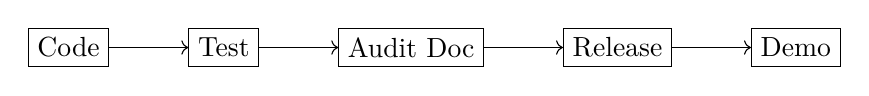
\begin{tikzpicture}
        \node[draw] (code) {Code};
        \node[draw, right=of code] (test) {Test};
        \node[draw, right=of test] (audit) {Audit Doc};
        \node[draw, right=of audit] (release) {Release};
        \node[draw, right=of release] (demo) {Demo};
        \draw[->] (code) -- (test);
        \draw[->] (test) -- (audit);
        \draw[->] (audit) -- (release);
        \draw[->] (release) -- (demo);
    \end{tikzpicture}
    \caption{Pipeline Packaging}
\end{figure}

\chapter{ÉLÉMENTS DE DIFFÉRENCIATION}

\section{Le Paradigme « Senior-by-Design »}

Le terme "Junior" est banni de notre vocabulaire. Un étudiant RBK ne sort pas pour "apprendre le métier", mais pour "exécuter le métier".
L'objectif est de produire un ingénieur immédiatement opérationnel, capable de livrer du code sécurisé en production sans supervision constante.

\paragraph{Mécanisme Opérationnel}
\begin{itemize}
    \item \textbf{No-AI Piscine :} Le filtre d'entrée se fait à la dure (Rust pur, sans Copilot) pour garantir la capacité cognitive.
    \item \textbf{Standards Audit :} Dès la semaine 9, tout code est soumis aux standards des cabinets d'audit (Documentation, Tests, Invariants).
    \item \textbf{Autonomie Radicale :} Pas de "prof" qui corrige. Peer-review et documentation technique sont les seules sources de vérité.
\end{itemize}

\begin{table}[h]
    \caption{Grille de Maturité Senior-by-Design}
    \centering
    \small
    
    \begin{tabular}{|p{2.5cm}|p{3cm}|p{4cm}|p{3.5cm}|}
        \hline
        \textbf{Axe} & \textbf{Niveau 0 (Junior)} & \textbf{Niveau 4 (Senior RBK)} & \textbf{Preuve} \\ \hline
        Architecture & Code monolithique & Modulaire, Composabilité & Diagramme C4 \\ \hline
        Sécurité & "Ça marche" & "C'est incassable" & Threat Model \\ \hline
        Tests & Manuels & CI/CD, Fuzzing, Property-Based & Rapport Coverage \\ \hline
        Collaboration & Solo coder & Reviewer implacable & Historique PR \\ \hline
    \end{tabular}
\end{table}

\begin{figure}[h]
    \centering
    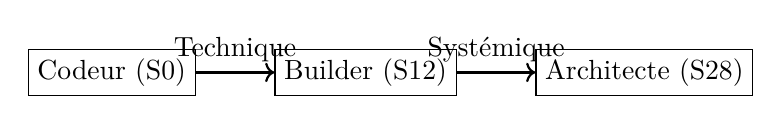
\begin{tikzpicture}
        \node[draw, rectangle] (coder) {Codeur (S0)};
        \node[draw, rectangle, right=of coder] (builder) {Builder (S12)};
        \node[draw, rectangle, right=of builder] (architect) {Architecte (S28)};
        \draw[->, thick] (coder) -- node[above] {Technique} (builder);
        \draw[->, thick] (builder) -- node[above] {Systémique} (architect);
    \end{tikzpicture}
    \caption{Transformation Codeur $\to$ Architecte}
\end{figure}

\section{Approche « Cyborg » : IA-Augmented Engineering}

L'IA n'est pas une béquille, c'est un exosquelette. Chez RBK, nous formons des "Cyborgs" : des ingénieurs qui utilisent l'IA pour multiplier leur productivité par 10, tout en gardant le contrôle absolu sur la qualité et la sécurité.

\paragraph{Protocole d'Usage}
\begin{itemize}
    \item \textbf{Autorisé :} Documentation, boilerplate, génération de tests unitaires, explication d'erreurs.
    \item \textbf{Interdit :} Copier-coller de logique métier critique sans audit ligne par ligne.
    \item \textbf{Traçabilité :} Tout prompt générant du code prod doit être loggé (Git commit message ou comments).
\end{itemize}

\begin{table}[h]
    \caption{Checklist d'Audit Code IA}
    \centering
    \small
    \begin{tabular}{|p{4cm}|l|l|}
        \hline
        \textbf{Point de Contrôle} & \textbf{Risque IA} & \textbf{Validation Humaine} \\ \hline
        Logique Invariante & Hallucination de règles métier & Preuve mathématique \\ \hline
        Vecteurs d'Attaque & Oubli de "Reentrancy Guard" & Analyse statique \\ \hline
        Edge Cases & Gestion naïve des erreurs & Tests de limites \\ \hline
    \end{tabular}
\end{table}

\section{Dual Track Solana/EVM : Flexibilité Stratégique}

Pourquoi choisir ? Le marché valorise la polyvalence. Nos ingénieurs sont "T-Shaped" : experts profonds sur une stack (ex: Solana) et compétents sur l'autre (EVM). Cela garantit une employabilité maximale et une capacité à auditer des architectures cross-chain.

\begin{table}[h]
    \caption{Comparatif Technique Solana vs EVM}
    \centering
    \small
    \begin{tabular}{|l|p{5cm}|p{5cm}|}
        \hline
        \textbf{Dimension} & \textbf{Solana (Track A)} & \textbf{EVM (Track B)} \\ \hline
        Modèle Mental & Stateless (Account Model) & Stateful (Contract Storage) \\ \hline
        Langage & Rust + Anchor & Solidity + Foundry \\ \hline
        Performance & Parallélisme (SVM) & Séquentiel (EVM) \\ \hline
        Sécurité & Ownership checks & Reentrancy guards \\ \hline
    \end{tabular}
\end{table}

\section{Intégration Superteam : Opportunités Directes}

Superteam n'est pas un partenaire, c'est notre client. RBK est conçu comme une usine à talents pour l'écosystème Superteam (Bounties, Grants, Jobs).

\paragraph{Processus}
\begin{enumerate}
    \item \textbf{Sourcing :} Les meilleurs bounties sont sélectionnés chaque lundi.
    \item \textbf{Squads :} Des équipes de 2-3 étudiants se forment pour attaquer les bounties complexes.
    \item \textbf{Review RBK :} Un mentor senior valide la soumission avant envoi (Quality Gate).
    \item \textbf{Revenue :} 100\% des gains vont aux étudiants (preuve de concept économique).
\end{enumerate}

\section{« On-Chain Resume » : Preuve de Travail Public}

Le CV PDF est mort. RBK délivre un "On-Chain Resume" vérifiable cryptographiquement.
Chaque compétence validée, chaque projet livré, chaque audit réalisé est ancré sur la blockchain via des SBT (Soulbound Tokens) et un historique GitHub immuable.

\begin{table}[h]
    \caption{Structure du On-Chain Resume}
    \centering
    \small
    \begin{tabularx}{\textwidth}{|l|l|X|}
        \hline
        \textbf{Composant} & \textbf{Support} & \textbf{Preuve Vérifiable} \\ \hline
        Identité & Wallet & Signature cryptographique \\ \hline
        Compétences & SBT Badge & Transaction on-chain (Issuer: RBK) \\ \hline
        Projets & GitHub Repo & Commit history, CI logs \\ \hline
        Réputation & DAO Vote & Poids de vote on-chain \\ \hline
    \end{tabularx}
\end{table}

\section{Ancrage Tunisie + Export : Software Factory Future}

RBK positionne la Tunisie comme la "Base Arrière" de l'ingénierie Web3 mondiale.
Moins cher que l'Europe de l'Est, plus qualifié que l'Asie du Sud-Est (sur la niche Rust/Crypto), et sur le même fuseau horaire que Paris/Berlin/Lagos.

\begin{table}[h]
    \caption{Risk Register Export}
    \centering
    \small
    \begin{tabular}{|l|l|p{6cm}|l|}
        \hline
        \textbf{Risque} & \textbf{Prob.} & \textbf{Impact} & \textbf{Mitigation} \\ \hline
        Juridique & Moyen & Blocage paiements & Contrats types validés, Crypto-payments \\ \hline
        Fuite Talents & Haut & Perte expertise locale & Modèle "Remote from Tunisia" (Salaire indexé) \\ \hline
        Qualité & Moyen & Perte réputation & QA systématique par Senior RBK \\ \hline
    \end{tabular}
\end{table}

\subsection{Comparatif RBK 2.0 vs Bootcamps Classiques}

RBK n'est pas un bootcamp. C'est un centre d'entraînement olympique pour ingénieurs.

\begin{table}[h]
    \caption{Matrice Comparée}
    \centering
    \small
    \begin{tabular}{|l|p{3.5cm}|p{3.5cm}|p{3.5cm}|}
        \hline
        \textbf{Critère} & \textbf{RBK 2.0} & \textbf{Bootcamp Web2} & \textbf{Université} \\ \hline
        Profondeur & Expert (Rust/Systems) & Surface (JS/React) & Théorique \\ \hline
        Sécurité & Obsessionnelle & Basique & Abstraite \\ \hline
        Preuve & Audit Report & "Projet TodoList" & Diplôme Papier \\ \hline
        Modèle Éco & ISA (Success fee) & Cash Upfront & Gratuit / Public \\ \hline
    \end{tabular}
\end{table}

\chapter{CONCLUSION \& FEUILLE DE ROUTE}

\section{Priorités Immédiates (Semaine 1–4)}

Le compte à rebours est lancé. Voici le plan d'attaque pour les 30 premiers jours post-validation de ce Whitepaper.

\begin{center}
    \textbf{Table: Plan 4 Semaines} \\
    \small
    \begin{tabular}{|l|l|p{4cm}|l|}
        \hline
        \textbf{Semaine} & \textbf{Objectif} & \textbf{Actions Clés} & \textbf{Owner} \\ \hline
        S1 & Légal & Validation Contrats ISA + Setup Bancaire & CEO \\ \hline
        S2 & Tech & Déploiement LMS + Setup Github Org & CTO \\ \hline
        S3 & Marketing & Lancement Landing Page + Campagne "Genesis" & CMO \\ \hline
        S4 & Ops & Ouverture Candidatures (Piscine Beta) & Ops \\ \hline
    \end{tabular}
\end{center}

\section{KPI de Succès}

Nous ne pilotons pas à vue. 12 indicateurs clés définissent la santé du projet.

\begin{center}
    \textbf{Table: KPI Dictionary (Extrait)} \\
    \small
    \begin{tabular}{|l|p{4cm}|l|l|}
        \hline
        \textbf{KPI} & \textbf{Définition} & \textbf{Cible S12} & \textbf{Seuil Alerte} \\ \hline
        Selectivity & \% Candidats admis piscine & < 10\% & > 20\% \\ \hline
        Attrition & \% Dropout durant piscine & < 30\% & > 50\% \\ \hline
        Job Ready & \% Certifiés "Audit-Ready" & > 80\% & < 60\% \\ \hline
        Placement & \% en poste à J+90 & > 70\% & < 50\% \\ \hline
    \end{tabular}
\end{center}

\section{Engagement Qualité Formel}

RBK s'engage sur une politique "Zéro Complaisance".
\begin{itemize}
    \item \textbf{Pas de diplôme de complaisance :} Si le niveau n'est pas atteint, l'étudiant double ou sort.
    \item \textbf{Code Review systématique :} Aucun code ne part en prod (ou validation) sans review par un pair et un mentor.
    \item \textbf{Transparence totale :} Les statistiques de placement et de salaire sont publiées et auditées.
\end{itemize}

\section{Forge de l'Élite Africaine}

RBK a l'ambition de devenir le "MIT du Web3" pour l'Afrique. Nous ne formons pas des exécutants bon marché, mais l'élite technologique qui construira l'infrastructure financière souveraine du continent.

\begin{center}
    \textbf{[Schéma: Flywheel RBK]} \\
    (Sélection $\to$ Formation $\to$ Preuves $\to$ Revenus $\to$ Réputation $\to$ Sélection)
\end{center}

\section{Synthèse Valeur Stratégique}

\begin{itemize}
    \item \textbf{Pour l'Étudiant :} Une carrière internationale à haute valeur ajoutée, sans dette initiale (ISA).
    \item \textbf{Pour l'Écosystème :} Un pipeline fiable de talents "Audit-Ready".
    \item \textbf{Pour la Tunisie :} Une entrée de devises forte et une montée en gamme technologique.
\end{itemize}

\section{Appel à l'Action}

Le marché n'attend pas. La fenêtre d'opportunité Solana/Rust est ouverte maintenant.
\textbf{Rejoignez la Cohorte Genesis.}

\begin{tcolorbox}[colback=SolanaPurple!5!white,colframe=SolanaPurple!75!black,title=Next Steps]
\begin{itemize}
    \item \textbf{[J0]} Validation Finale Whitepaper.
    \item \textbf{[J+7]} Lancement Recrutement Core Team.
    \item \textbf{[J+30]} Ouverture des Candidatures.
\end{itemize}
\end{tcolorbox}

\section{Message Final au CEO}

Monsieur le CEO,
Ce plan est ambitieux, risqué, mais nécessaire. Il transforme RBK d'un centre de formation classique en une \textbf{Startup Studio Éducative}.
Le modèle économique est viable (ISA + Bounties). La demande marché est validée. La technologie est mature.
Il ne reste qu'une variable : l'Exécution.
C'est un \textbf{GO}.

\section{Profil de Sortie}

\begin{center}
    \textbf{Table: Profil de Sortie Standard} \\
    \small
    \begin{tabular}{|l|p{4cm}|l|}
        \hline
        \textbf{Compétence} & \textbf{Preuve} & \textbf{Seuil} \\ \hline
        Rust / Solana & 3 Repos GitHub Clean & CI Green \\ \hline
        Sécurité & 1 Rapport d'Audit & 3 vulns trouvées \\ \hline
        Soft Skills & Démo Vidéo & Clarté > 4/5 \\ \hline
    \end{tabular}
\end{center}


% --- LISTES ---
\listoffigures
\listoftables

\clearpage
\phantomsection
\addcontentsline{toc}{part}{ANNEXES}
\appendix
\chapter{SYLLABUS TECHNIQUE DÉTAILLÉ (28 SEMAINES)}

\section{Structure Hebdomadaire Standard}

Chaque semaine suit le rythme : Concept (Lun) $\to$ Lab Guidé (Mar) $\to$ Projet Solo (Mer-Jeu) $\to$ Audit/Demo (Ven).

\begin{center}
    \textbf{Table: Syllabus Synthétique} \\
    \small
    \begin{tabular}{|c|p{4cm}|p{5cm}|p{2.5cm}|}
        \hline
        \textbf{Sem} & \textbf{Objectif} & \textbf{Livrable} & \textbf{DoD} \\ \hline
        \multicolumn{4}{|c|}{\textbf{PHASE 0 : PISCINE RUST (S1-S4)}} \\ \hline
        S1 & Syntaxe & CLI Todo List & Exécutable \\ \hline
        S2 & Memory Management & Linked List & Leak-free \\ \hline
        S3 & Concurrency & Mini Web Server & Multithreaded \\ \hline
        S4 & Search Engine & Grep-like Tool & Perf < 10ms \\ \hline
        \multicolumn{4}{|c|}{\textbf{PHASE 1 : FONDATIONS WEB3 (S5-S12)}} \\ \hline
        S5 & Cryptographie & Hash/Sign Tools & Std compliant \\ \hline
        S6 & Solana Model & Raw Transaction Script & Executable \\ \hline
        \multicolumn{4}{|c|}{\textbf{PHASE 2 : SPÉCIALISATION (S13-S24)}} \\ \hline
        S13 & Anchor Framework & Basic Vault & Secure \\ \hline
        S20 & Security Deep Dive & Hacking Challenge & Flag Captured \\ \hline
        \multicolumn{4}{|c|}{\textbf{PHASE 3 : PROFESSIONNALISATION (S25-S28)}} \\ \hline
        S28 & Final Demo & Production Release & Audit Approved \\ \hline
    \end{tabular}
\end{center}

\section{Rubrique d'Évaluation Hebdo}
(Voir texte section suivante)

\chapter{MODÈLE FINANCIER DÉTAILLÉ}

Le modèle financier RBK 2.0 repose sur une approche **Hybride** robuste, privilégiant la liquidité immédiate via les frais Upfront tout en conservant un potentiel d'upside significatif via l'ISA pour les Top Talents.

\section{Hypothèses Structurantes}

Nous retenons le **Scénario Hybride** comme base du Business Plan.

\begin{center}
    \textbf{Structure de Revenus (Cible)} \\
    \small
    \rowcolors{2}{gray!5}{white}
    \begin{tabularx}{\textwidth}{|l|X|l|}
        \hline
        \textbf{Flux} & \textbf{Description} & \textbf{Part du Volume} \\ \hline
        \textbf{Upfront (B2C)} & Paiement direct par les étudiants (Niveaux 1, 2, 3 ou Pack). Assure le BFR immédiat. & \textbf{60\%} des étudiants \\ \hline
        \textbf{ISA (Différé)} & Paiement différé 15\% sur 36 mois. Option réservée aux profils "Top Potential" (N3/Pack). & \textbf{30\%} des étudiants \\ \hline
        \textbf{Services (B2B)} & Formation d'employés et placement, payé par les entreprises (Sponsoring/Hiring). & \textbf{10\%} des revenus \\ \hline
    \end{tabularx}
\end{center}

\section{Paramètres ISA \& Cash Drag}

L'option ISA introduit un décalage de trésorerie ("Cash Drag") que notre modèle anticipe :
\begin{itemize}
    \item \textbf{Taux de Placement :} Hypothèse conservatrice de **85\%** des étudiants ISA placés à 6 mois.
    \item \textbf{Délai de Paiement :} 
    \begin{itemize}
        \item Formation : 6 mois (Cycle complet).
        \item Recherche d'emploi : 3 mois (Moyenne).
        \item \textbf{Premier versement ISA :} À M+10 après le démarrage.
    \end{itemize}
    \item \textbf{Impact :} Les revenus ISA de l'Année 1 sont quasi nuls (amorçage). Ils deviennent significatifs en Année 2 (effet cumulatif des cohortes précédentes).
\end{itemize}

\section{Modèle Tarifaire (Base de calcul)}
Pour les besoins de la modélisation :
\begin{itemize}
    \item \textbf{Panier Moyen Upfront :} Estimé à \textbf{12 000 TND} (Mix pondéré : N1 seul, N1+N2 et Pack Complet Upfront).
    \item \textbf{Revenu Moyen ISA :} Estimé à \textbf{18 900 TND} (basé sur salaire moyen net 3 500 TND sur 36 mois : 525 x 36).
    \item \textbf{Marge Nette par Étudiant :} Cible > 35\% après coûts mentors et infrastructure.
\end{itemize}

\section{Unit Economics (Par Étudiant)}
\begin{center}
    \small
    \begin{tabular}{|l|r|l|}
        \hline
        \textbf{Poste} & \textbf{Montant (TND)} & \textbf{Note} \\ \hline
        \textbf{Revenu Moyen (A)} & \textbf{12 000} & Mix Upfront/ISA pondéré \\ \hline
        Mentorat (Variable) & (1 500) & Ratio expert 1:12 \\ \hline
        Infrastructure & (300) & Serveurs, SaaS, Licences \\ \hline
        Acquisition (CAC) & (500) & Marketing digital \\ \hline
        \textbf{Total Coût Variable (B)} & \textbf{(2 300)} & COGS \\ \hline
        \textbf{Marge Contributive (A-B)} & \textbf{9 700} & \textbf{80\% de Marge Brute} \\ \hline
    \end{tabular}
\end{center}

\section{Rentabilité \& Seuil}
Le seuil de rentabilité opérationnelle (Breakeven) est atteint dès que le volume dépasse **40 étudiants payants / an** (Niveau 1+), ce qui sécurise la structure indépendamment des succès ISA.

\chapter{ANNEXE — CADRE JURIDIQUE \&\\ CONFORMITÉ (TUNISIE)}
\label{ann:juridique}

\section{Synthèse Juridique : Opérer depuis la Tunisie}
Grâce au statut Entreprise Totalement Exportatrice (ETE), l'ingénieur RBK bénéficie d'une exonération fiscale massive sur ses revenus étrangers (0\% IS pendant 4 ans, puis 10\%). Ce cadre, couplé à une gestion rigoureuse des flux crypto/fiat, fait de la Tunisie un hub Web3 ultra-compétitif.

\section{Statut d'Entreprise Totalement\\ Exportatrice (ETE)}

Nous rappelons ici le cadre légal tunisien qui permet d'opérer en devises tout en restant conforme.

\subsection{Définition et Cadre Légal}
L'Entreprise Totalement Exportatrice (ETE) est un régime fiscal tunisien réglementé par le Code d'Incitation aux Investissements (Loi n°2016-71) et le Décret n°2017-758. Il permet aux entités réalisant 100\% de leur chiffre d'affaires à l'export de bénéficier d'avantages majeurs.

\section{Avantages Fiscaux}
\begin{itemize}
	\item \textbf{Impôts Sociétés (IS) :} Exonération totale pendant 4 ans, puis taux réduit à 10\% (vs 15\% standard).
	\item \textbf{Confidentialité B2B :} Pour tout contrat international, signer un \RBKTerm{nda} précisant périmètre et durée.
	\item \textbf{Devises :} Liberté totale de gestion des comptes en devises étrangères (EUR/\RBKTerm{usd}) sans autorisation préalable de la BCT pour les opérations liées à l'activité.
	\item \textbf{TVA :} Exonération de TVA sur les services et biens acquis pour l'exportation (en suspension de taxes).
	\item \textbf{Dividendes :} Exonération de retenue à la source sur les dividendes distribués.
\end{itemize}

\subsection{Conditions d'Éligibilité pour RBK 2.0}
Pour bénéficier du statut ETE, RBK (et ses alumni entrepreneurs) doit :
\begin{itemize}
	\item Exporter 100\% de ses services à l'étranger (formation remote, consulting, audit).
	\item Justifier d'un plan d'affaires et créer un minimum d'emplois.
\end{itemize}

\subsection{Avantages Fiscaux Comparés}
\begin{table}[H]
	\caption{Comparatif Fiscal : Standard vs ETE}
	\centering
	\begin{tabularx}{\textwidth}{|l|l|Y|}
		\hline
		\textbf{Indicateur} & \textbf{Régime Standard} & \textbf{Régime ETE (Export)}   \\ \hline
		IS (Impôt Sociétés) & 15\% dès Année 1         & 0\% (4 ans) puis 15\%          \\ \hline
		Dividendes          & Retenue à la source 10\% & Exonérés (si bénéfices export) \\ \hline
		TVA Achats          & 19\%                     & Suspension de TVA              \\ \hline
		Compte Bancaire     & TND uniquement           & Devises + TND                  \\ \hline
	\end{tabularx}
\end{table}

\section{Kit de Survie Juridique Freelance}

Cette section offre des réflexes juridiques rapides pour sécuriser les missions internationales.

\subsection{Matrice de Décision : Patente vs SUARL}
\begin{table}[H]
	\centering
	\begin{tabularx}{\textwidth}{|l|Y|Y|}
		\hline
		\textbf{Critère} & \textbf{Patente (Pers. Physique)} & \textbf{SUARL (Pers. Morale)} \\ \hline
		Coût Création    & Quasi-nul                         & Moyen (1000 TND + Capital)    \\ \hline
		Complexité       & Très faible                       & Moyenne                       \\ \hline
		Responsabilité   & Illimitée                         & Limitée au capital            \\ \hline
		Recommandation   & Pour débuter (< 50k TND/an)       & Dès que \RBKTerm{ca} > 80k TND/an       \\ \hline
	\end{tabularx}
\end{table}

\subsection{Checklist Création d'Entreprise ETE}
\begin{enumerate}
	\item[{\faIcon[regular]{square}}] J-0 : Rédaction des statuts (Objet social : "Export de services informatiques").
	\item[{\faIcon[regular]{square}}] J-2 : Dépôt dossier APII en ligne (Déclaration d'investissement).
	\item[{\faIcon[regular]{square}}] J-15 : Obtention de l'attestation de dépôt APII.
	\item[{\faIcon[regular]{square}}] J-20 : Enregistrement Recette Finance (Timbre fiscal).
	\item[{\faIcon[regular]{square}}] J-30 : Immatriculation RNE (Registre National des Entreprises).
	\item[{\faIcon[regular]{square}}] J-35 : Ouverture Compte Bancaire "Dossier Juridique" (+ Compte Devises).
\end{enumerate}

\section{Mécanisme de Paiement\\ \texorpdfstring{Crypto $\to$ Fiat}{Crypto -> Fiat} Conforme}

Nous décrivons le chemin de paiement recommandé pour rester traçable et compatible avec les exigences bancaires.

\subsection{Traçabilité Comptable}
Pour chaque transaction entrante :
\begin{enumerate}
	\item Émettre une facture en Devises (EUR/\RBKTerm{usd}) mentionnant "Règlement par voie électronique".
	\item Conserver le "Transaction Hash" comme preuve d'exécution.
	\item Obtenir l'avis de crédit bancaire mentionnant l'origine des fonds (Bitwage/Grey).
	\item Comptabiliser en TND au taux du jour de réception.
\end{enumerate}

\section{Validation Juridique des ISA}

Ce passage précise les garde-fous qui rendent les ISA applicables dans le contexte tunisien.

\subsection{Qualification Juridique (COC)}
Le contrat ISA est qualifié de Contrat Innommé (Article 2 du Code des Obligations et Contrats), régi par la volonté des parties tant qu'il ne contrevient pas à l'ordre public. Il s'apparente à :
\begin{itemize}
	\item Un Prêt à Rémunération Variable.
	\item Un contrat de Musharaka (Finance islamique).
\end{itemize}

\subsection{Risques Juridiques \& Mitigation}
\begin{table}[H]
	\caption{Matrice des Risques Principaux}
	\centering
	\begin{tabularx}{\textwidth}{|l|l|l|Y|}
		\hline
		\textbf{Risque}     & \textbf{Prob.} & \textbf{Imp.} & \textbf{Mitigation}                              \\ \hline
		Requalification ISA & Moy.           & Élevé         & Cap à 1.5x, durée limitée, validation avocat.    \\ \hline
		Blocage Crypto      & Faible         & Critique      & Alternative TND + Structure Offshore de secours. \\ \hline
	\end{tabularx}
\end{table}

\section{Plan de Continuité Juridique}
\begin{itemize}
	\item \textbf{Scénario 1 : Changement réglementaire défavorable.} Action : Bascule 100\% TND via partenaires bancaires locaux. Migration de l'entité légale IP à l'étranger.
	\item \textbf{Scénario 2 : Défaut massif ISA (>30\%).} Action : Activation du Fonds de Garantie (50k TND). Restructuration des dettes.
\end{itemize}

\chapter{TEMPLATE DE RAPPORT D'AUDIT DE SÉCURITÉ}

Un rapport d'audit professionnel doit être clair, complet et actionnable.

\section{Structure du Rapport}
\begin{enumerate}
    \item \textbf{Executive Summary :} Résumé pour les décideurs (Score, Risque global).
    \item \textbf{Scope :} Liste des fichiers audités et Commit Hash.
    \item \textbf{Findings :} Liste des vulnérabilités classées par sévérité.
    \item \textbf{Recommendations :} Conseils d'architecture généraux.
\end{enumerate}

\section{Classification des Risques}

\begin{center}
    \textbf{Table: Échelle de Sévérité} \\
    \small
    \begin{tabular}{|l|l|p{6cm}|}
        \hline
        \textbf{Niveau} & \textbf{Impact} & \textbf{Exemple} \\ \hline
        \textbf{CRITICAL} & Perte de fonds directe, Gel définitif & Reentrancy, Owner Key compromise \\ \hline
        \textbf{HIGH} & Dégradation sévère du service, Perte partielle & DoS, Price Oracle manipulation \\ \hline
        \textbf{MEDIUM} & Grief mineur, Coût Gas élevé & Griefing attack, Unbounded Loop \\ \hline
        \textbf{LOW/INFO} & Bonnes pratiques, Lisibilité & Typo, Dead code \\ \hline
    \end{tabular}
\end{center}

\section{Fiche Finding Type}

\begin{tcolorbox}[title=ID-01 : Unchecked External Call (H-01)]
\textbf{Sévérité :} HIGH \\
\textbf{Fichier :} \texttt{vault.rs} \\
\textbf{Description :} L'appel CPI vers le programme Token ne vérifie pas le code retour.
\textbf{Impact :} Un attaquant peut forcer l'échec silencieux du transfert et créditer son solde interne.
\textbf{Recommandation :} Utiliser \texttt{anchor\_lang::solana\_program::program::invoke\_signed} et gérer le \texttt{Result}.
\end{tcolorbox}

\chapter{LE COCKPIT DE L'ARCHITECTE}

Liste des outils obligatoires pour un étudiant en phase de production.

\section{Stack Outillage Minimal}

\begin{center}
    \textbf{Table: Cockpit Tools} \\
    \small
    \begin{tabular}{|l|l|p{6cm}|}
        \hline
        \textbf{Outil} & \textbf{Usage} & \textbf{Output Attendu} \\ \hline
        \textbf{Obsidian/Notion} & Knowledge Base & Wiki du projet, Notes de recherche \\ \hline
        \textbf{Excalidraw} & Diagramming & Schémas d'architecture C4 \\ \hline
        \textbf{Linear/Jira} & Task Management & Tickets spécifiés et trackés \\ \hline
        \textbf{Cursor/VSCode} & IDE & Code avec Linter et Copilot configuré \\ \hline
    \end{tabular}
\end{center}

\section{Journée Type (Productivité)}

\begin{itemize}
    \item \textbf{09h-12h (Deep Work) :} Coding (Feature complexe ou Refactoring). Pas de notifs.
    \item \textbf{13h-14h (Review) :} Code Review des PRs des collègues.
    \item \textbf{14h-16h (Ops) :} Tests, Documentation, Fixes mineurs.
    \item \textbf{16h-17h (Sync) :} Daily Standup, Synchro Architecte.
\end{itemize}

\chapter{ANNEXE — Modèle ISA (Income Share Agreement)}
\label{ann:isa}

\section{Objet et Principes}
L'ISA est un mécanisme de financement sélectif destiné à aligner l'école et l'étudiant : l'étudiant ne paie que s'il dépasse un seuil de revenu, et l'école accepte un risque. L'ISA est réservé aux profils validés Top Talent.

\section{Éligibilité (Gating)}
\begin{itemize}
    \item \textbf{Périmètre :} réservé au parcours complet (N1+N2+N3).
    \item \textbf{Quota :} nombre de places ISA limité par cohorte (ex : 30\% max).
    \item \textbf{Sélection :} top performance + validation par comité.
\end{itemize}

\section{Définitions Normalisées (Net/Brut)}
\begin{itemize}
    \item \textbf{Revenu Net Mensuel (RNM) :} Montant net effectivement perçu et traçable.
    \item \textbf{Seuil de Déclenchement :} 3 000 TND nets / mois.
    \item \textbf{Taux de Partage :} 15\% du RNM (si > Seuil).
    \item \textbf{Cap (Plafond) :} 20 000 TND total.
    \item \textbf{Durée Maximale :} 36 mensualités de paiement maximum ou 60 mois calendaires.
\end{itemize}

\section{Règles de Pause, Chômage, Variabilité}
\begin{itemize}
    \item \textbf{Pause automatique :} si RNM <= 3 000, paiement = 0.
    \item \textbf{Reprise :} dès que RNM > 3 000.
    \item \textbf{Variabilité :} aucun rattrapage sur les mois faibles.
\end{itemize}

\section{Cas Limites (Edge Cases)}
\begin{enumerate}
    \item \textbf{RNM fluctuant :} paiement déclenché uniquement les mois > Seuil.
    \item \textbf{Plusieurs revenus :} RNM = somme des nets traçables.
    \item \textbf{Départ à l'étranger :} conversion en TND au taux mensuel.
\end{enumerate}

\section{Conformité Éthique (Musharaka)}
Le modèle est compatible finance participative : Partage de Risque (Perte pour l'école si échec) et Partage de Profit minoritaire.

\section{Exemples Chiffrés (Seuil 3 000 net, Taux 15\%)}
\begin{table}[H]
    \caption{Scénarios de Remboursement}
    \centering
    \begin{tabularx}{\textwidth}{|l|l|l|X|}
        \hline
        \textbf{Scénario} & \textbf{RNM} & \textbf{Mensualité} & \textbf{Statut Final} \\ \hline
        A. Junior local & 3 500 & 525 & Arrêt à 36 mois (< Cap) \\ \hline
        B. Profil solide & 5 000 & 750 & Cap atteint au 27ème mois \\ \hline
        C. Remote & 6 000 & 900 & Cap atteint au 23ème mois \\ \hline
        D. Chômage & 0 & 0 & Drop-off à 60 mois (0 TND) \\ \hline
    \end{tabularx}
\end{table}

\chapter{GUIDE DE SÉLECTION \& SCORING « PISCINE RUST »}

La Piscine n'est pas un cours, c'est un filtre.

\section{Grille de Scoring}

Le score final (sur 100) détermine l'admission. Seuil d'admission : 75/100.

\begin{center}
    \textbf{Table: Critères de Sélection} \\
    \small
    \begin{tabular}{|l|r|p{8cm}|}
        \hline
        \textbf{Critère} & \textbf{Poids} & \textbf{Indicateurs} \\ \hline
        \textbf{Aptitude Tech} & 40\% & Progression sur les exercices Rust, Qualité du code final. \\ \hline
        \textbf{Résilience} & 30\% & Capacité à rebondir après échec, Constance de l'effort. \\ \hline
        \textbf{Collaboration} & 20\% & Aide apportée aux autres (Peer-learning). \\ \hline
        \textbf{Communication} & 10\% & Clarté des questions posées, Respect des mentors. \\ \hline
    \end{tabular}
\end{center}

\section{Red Flags (Éliminatoires)}
\begin{itemize}
    \item \textbf{Plagiat / Triche :} Copie de code sans compréhension, usage caché d'IA. $\to$ Exclusion immédiate.
    \item \textbf{Toxicité :} Comportement agressif ou dénigrant envers pairs/mentors.
    \item \textbf{Fantôme :} Absence non justifiée > 2 jours.
\end{itemize}

\section{Admission Parallèle (Accès Direct N2 / N3)}

Pour les profils expérimentés souhaitant "sauter" le tronc commun ou la spécialisation, nous proposons un processus d'admission spécifique visant à valider les acquis de manière irréfutable.

\subsection{Test d'Entrée Niveau 2 (Bypass Piscine)}
\textbf{Pré-requis :} Maîtrise prouvée de Rust ou C++ et des concepts Blockchain de base.

\begin{enumerate}
    \item \textbf{Théorie (45 min) :} QCM statique sur l'Account Model, le Memory Management (Stack/Heap) et la Complexité Algorithmique.
    \item \textbf{Pratique (3h) :} "Mini-Piscine Express". Implémentation d'une CLI Rust qui parse un fichier binaire et signe une payload cryptographique (Ed25519). \textbf{Critère Éliminatoire :} Absence de tests unitaires ou usage d'IA générative détecté.
    \item \textbf{Entretien (15 min) :} Code review live avec le Lead Instructor. Justification des choix d'allocation mémoire.
\end{enumerate}

\begin{table}[h]
    \caption{Barème Admission N2}
    \centering
    \small
    \begin{tabularx}{\textwidth}{|l|l|X|l|}
        \hline
        \textbf{Critère} & \textbf{Points} & \textbf{Attendu} & \textbf{KO si...} \\ \hline
        Code Quality & 40 & Rust idiomatique, Zero CLippy warnings & `unwrap()` non géré \\ \hline
        Tests & 30 & Unit tests couvrant les edge cases & 0 tests \\ \hline
        Architecture & 30 & Gestion erreurs (Result), Structs propres & Code non structuré \\ \hline
    \end{tabularx}
\end{table}

\subsection{Test d'Entrée Niveau 3 (Bypass Track)}
\textbf{Pré-requis :} Portfolio prouvant 2+ ans d'expérience sur la stack cible (Solana ou EVM).

\begin{enumerate}
    \item \textbf{Audit Readiness :} Soumission d'un repo personnel existant. Vérification des critères "Studio" (CI/CD, Docs, Tests E2E).
    \item \textbf{Exercice de Review :} L'étudiant doit auditer une PR contenant 3 vulnérabilités cachées (Reentrancy, Arithmetic Overflow, Access Control).
\end{enumerate}

\chapter{SPÉCIFICATIONS TECHNIQUES SBT}

\section{Schéma de Métadonnées (JSON)}

Les SBT RBK suivent le standard Metaplex Core ou ERC-721 (Non-Transferable).

\begin{lstlisting}[caption=Metadata SBT Standard]
{
  "name": "RBK Guardian - Cohort 1",
  "symbol": "RBKC1-G",
  "description": "Certified Solana Smart Contract Engineer.",
  "image": "https://arweave.net/...",
  "attributes": [
    { "trait_type": "Track", "value": "Solana" },
    { "trait_type": "Level", "value": "Gold" },
    { "trait_type": "Cohort", "value": "Genesis 2025" },
    { "trait_type": "FinalGrade", "value": "92/100" }
  ],
  "properties": {
    "files": [
      { "uri": "https://github.com/student/capstone", "type": "text/html" },
      { "uri": "https://rbk.tn/audit/S12345", "type": "application/pdf" }
    ]
  }
}
\end{lstlisting}

\section{Processus de Vérification}
\begin{enumerate}
    \item \textbf{Issuer Check :} Vérifier que l'adresse émettrice est bien le Multisig RBK Certifié.
    \item \textbf{Owner Check :} L'étudiant prouve qu'il possède le wallet (Signature message).
    \item \textbf{Content Check :} Le lien vers le rapport d'audit correspond au hash stocké on-chain.
\end{enumerate}

\chapter{DASHBOARD DE SUIVI PROMO}

\section{Indicateurs Hebdomadaires (KPI)}

\begin{center}
    \textbf{Table: Métriques de Santé Promo} \\
    \small
    \begin{tabular}{|l|l|p{4cm}|l|}
        \hline
        \textbf{Catégorie} & \textbf{KPI} & \textbf{Formule} & \textbf{Cible} \\ \hline
        Progression & Velocity & Nb exercices validés / Nb total & > 90\% \\ \hline
        Qualité & First Time Pass & \% Labs validés du 1er coup & > 50\% \\ \hline
        Engagement & Attendance & Taux présence Dailies & > 95\% \\ \hline
        Moral & NPS Hebdo & "Recommanderiez-vous cette semaine ?" & > 8/10 \\ \hline
    \end{tabular}
\end{center}

\section{Questionnaire Bien-être Minimal}
Envoyé chaque vendredi via Bot Discord (Anonyme).
\begin{enumerate}
    \item Niveau de stress (1-5) ?
    \item Charge de travail (Trop faible / OK / Trop forte) ?
    \item Sentiment de progression (Je stagne / J'apprends / Je vole) ?
\end{enumerate}
\chapter{OFFRE COMMERCIALE \& MODALITÉS}

\section{Le Pack RBK 2.0}

Ce qui est inclus pour chaque étudiant retenu.

\begin{center}
    \textbf{Table: Détail de l'Offre} \\
    \small
    \begin{tabular}{|p{8cm}|c|c|}
        \hline
        \textbf{Service} & \textbf{Standard} & \textbf{Inclus ?} \\ \hline
        Formation 48 semaines (N1+N2+N3) & 1800h+ & OUI \\ \hline
        Mentorat Expert (Review code hebdo) & Senior & OUI \\ \hline
        Certification SBT & On-chain & OUI \\ \hline
        Accès Réseau Partenaires & Superteam & OUI \\ \hline
        Hébergement (Piscine) & Optionnel & NON \\ \hline
    \end{tabular}
\end{center}

\section{Pricing \& Conditions (Value Ladder)}

Notre tarification est conçue pour réduire le risque à l'entrée via un système progressif.

\begin{table}[H]
    \caption{Grille Tarifaire (TND)}
    \centering
    \small
    \rowcolors{2}{gray!5}{white}
    \begin{tabularx}{\textwidth}{|l|l|l|X|}
        \hline
        \textbf{Niveau} & \textbf{Prix} & \textbf{Paiement} & \textbf{Inclus} \\ \hline
        \textbf{Niveau 1} (12 sem) & 2 900 TND & 2x 1 450 TND & Piscine + Fondations \\ \hline
        \textbf{Niveau 2} (16 sem) & 5 900 TND & 3x 1 966 TND & Spécialisation Track \\ \hline
        \textbf{Niveau 3} (20 sem) & 8 900 TND & 4x 2 225 TND & Pro-Audit-Placement \\ \hline
        \textbf{Pack Complet} & \textbf{15 900 TND} & \textbf{6x 2 650 TND} & \textbf{Tout inclus (N1-N3)} \\ \hline
    \end{tabularx}
\end{table}

\subsection{Mécanisme d'Incitation (Upgrade)}
\begin{itemize}
    \item \textbf{Crédit 100\% :} Si vous payez le N1 et décidez de continuer, les 2 900 TND sont déduits du Pack.
    \item \textbf{Fenêtre 30 jours :} L'upgrade doit se faire sous 30 jours pour verrouiller le tarif global.
\end{itemize}

\subsection{Admission Directe (Passerelles)}
\textbf{Accès direct N2 :} Possible via tests techniques obligatoires (Rust/Algo/Git). Frais de test : 200 TND (non remboursable, mais déduit si inscription).
\textbf{Accès direct N3 :} Strictement réservé aux profils expérimentés (Portfolio Web3 solide + Audit check). Test + Entretien. Frais : 300 TND.

\subsection{Offre ISA (Income Share Agreement)}
\textbf{Périmètre :} Réservé aux "Top Talents" sur le **Pack Complet** ou **Niveau 3**. Sélection stricte (Dossier + Technique + Social).
\textbf{Conditions Unifiées :}
\begin{itemize}
    \item \textbf{Partage :} 15\% du revenu brut mensuel.
    \item \textbf{Déclencheur (Threshold) :} Salaire > 2 500 TND Brut.
    \item \textbf{Durée :} 36 mensualités (paiements effectifs) maximum.
    \item \textbf{Plafond (Cap) :} 20 000 TND total remboursé (Risk Premium inclus).
    \item \textbf{Clause de pause :} Automatique en cas de chômage ou revenu < Seuil.
    \item \textbf{Juridiction :} Droit Tunisien, contrat enregistré.
\end{itemize}

\begin{figure}[H]
    \centering
    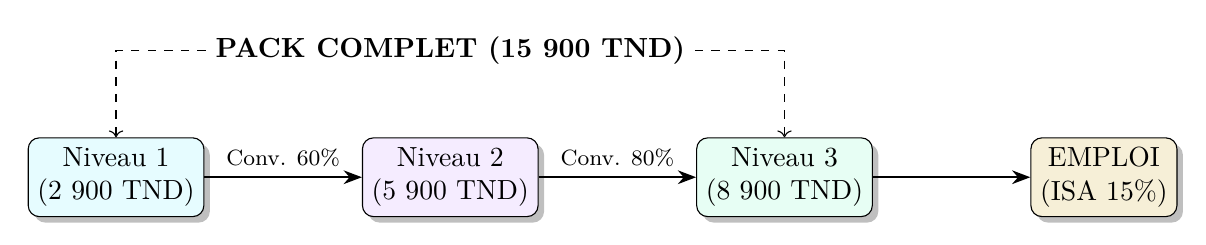
\begin{tikzpicture}[node distance=2cm, auto,
        block/.style={rectangle, draw, rounded corners, minimum height=1cm, align=center, fill=white, drop shadow},
        arrow/.style={->, >=Stealth, thick}]
        
        \node[block, fill=SolanaBlue!10] (n1) {Niveau 1\\(2 900 TND)};
        \node[block, fill=SolanaPurple!10, right=of n1] (n2) {Niveau 2\\(5 900 TND)};
        \node[block, fill=SolanaGreen!10, right=of n2] (n3) {Niveau 3\\(8 900 TND)};
        \node[block, fill=MF_Gold!20, right=of n3] (job) {EMPLOI\\(ISA 15\%)};
        
        \draw[arrow] (n1) -- node[above]{\footnotesize Conv. 60\%} (n2);
        \draw[arrow] (n2) -- node[above]{\footnotesize Conv. 80\%} (n3);
        \draw[arrow] (n3) -- (job);
        
        \node[above=0.8cm of n2] (bundle) {\textbf{PACK COMPLET (15 900 TND)}};
        \draw[dashed, ->] (bundle) -| (n1);
        \draw[dashed, ->] (bundle) -| (n3);
    \end{tikzpicture}
    \caption{Value Ladder et Parcours Étudiant}
\end{figure}

\section{Objections \& Réponses}
\textbf{"C'est trop cher ?"}
C'est le prix d'une voiture d'occasion pour une carrière internationale. L'option "Niveau 1" vous permet de tester pour un coût réduit.

\textbf{"Pourquoi pas une fac publique ?"}
La fac offre un diplôme académique. Nous offrons une certification technique industrielle et un accès direct au réseau Superteam.

\section{Politique de Remboursement et Report}
\begin{itemize}
    \item \textbf{Satisfait ou Remboursé (N1) :} Remboursement intégral possible jusqu'à la fin de la 1ère semaine du Niveau 1.
    \item \textbf{Report de Cohorte :} Possible une seule fois en cas de force majeure, sans frais, sous réserve de places disponibles.
    \item \textbf{Non-Garanti :} RBK s'engage sur la qualité de la formation ("Obligation de Moyens") mais ne peut garantir contractuellement une embauche ou un niveau de salaire spécifique ("Obligation de Résultats"), ceux-ci dépendant du marché et de l'effort individuel.
\end{itemize}

\chapter{GLOSSAIRE COMPLET}

\section{Concepts Fondamentaux Web3}

\begin{center}
    \small
    \rowcolors{2}{gray!5}{white}
    \renewcommand{\arraystretch}{1.4}
    \begin{tabularx}{\textwidth}{|l|X|}
        \hline
        \textbf{Terme} & \textbf{Définition} \\ \hline
        \textbf{Web3} & La 3ème itération d'Internet, décentralisée et basée sur la propriété numérique via la blockchain (vs Web2 dominé par les plateformes centralisées). \\ \hline
        \textbf{Blockchain} & Un registre numérique partagé, immuable et distribué qui enregistre les transactions et suit les actifs d'un réseau. \\ \hline
        \textbf{Smart Contract} & Programme informatique auto-exécutable stocké sur une blockchain qui s'exécute lorsque des conditions prédéfinies sont remplies. \\ \hline
        \textbf{DApp} & Application Décentralisée fonctionnant sur une blockchain via des Smart Contracts, sans serveur central de contrôle. \\ \hline
        \textbf{Tokenomics} & L'économie d'un token : son émission, sa distribution, son utilité et les mécanismes d'incitation financière. \\ \hline
        \textbf{DAO} & Organisation Autonome Décentralisée : Une entité gérée par du code (Smart Contracts) et gouvernée par ses membres via des tokens. \\ \hline
    \end{tabularx}
\end{center}

\section{Infrastructure \& Protocoles}

\begin{center}
    \small
    \rowcolors{2}{gray!5}{white}
    \renewcommand{\arraystretch}{1.4}
    \begin{tabularx}{\textwidth}{|l|X|}
        \hline
        \textbf{Terme} & \textbf{Définition} \\ \hline
        \textbf{Layer 1 (L1)} & Blockchain principale (ex: Solana, Ethereum) qui assure la sécurité et le consensus. \\ \hline
        \textbf{Layer 2 (L2) / Rollup} & Solution de mise à l'échelle construite "par-dessus" un L1 (ex: Ethereum) pour réduire les coûts et augmenter la vitesse. \\ \hline
        \textbf{EVM} & Ethereum Virtual Machine : L'environnement d'exécution standard d'Ethereum, utilisé aussi par de nombreuses autres chaînes (Polygon, Base). \\ \hline
        \textbf{SVM} & Solana Virtual Machine : Moteur d'exécution haute performance de Solana, capable de traiter des milliers de transactions en parallèle. \\ \hline
        \textbf{DePIN} & Decentralized Physical Infrastructure Networks : Utilisation de la blockchain pour gérer des infrastructures physiques (télécoms, énergie, GPU). \\ \hline
        \textbf{DeFi} & Finance Décentralisée : Services financiers (prêt, échange) sans intermédiaires bancaires. \\ \hline
        \textbf{Oracle} & Service tiers qui connecte les Smart Contracts aux données du monde réel (prix, météo). \\ \hline
        \textbf{Bridge} & Protocole permettant de transférer des actifs ou des données entre deux blockchains différentes. \\ \hline
    \end{tabularx}
\end{center}

\section{Terminologie Solana (Spécifique)}

\begin{center}
    \small
    \rowcolors{2}{gray!5}{white}
    \renewcommand{\arraystretch}{1.4}
    \begin{tabularx}{\textwidth}{|l|X|}
        \hline
        \textbf{Terme} & \textbf{Définition} \\ \hline
        \textbf{Account Model} & Modèle de données où tout est un "Compte" (Fichiers, Programmes, Données). Contraire au modèle UTXO de Bitcoin. \\ \hline
        \textbf{PDA} & Program Derived Address : Une adresse contrôlée par un programme (non par une clé privée), essentielle pour la sécurité et l'automatisation. \\ \hline
        \textbf{CPI} & Cross-Program Invocation : Capacité d'un programme à en appeler un autre (composabilité). \\ \hline
        \textbf{Sealevel} & Le moteur de parallélisation de Solana qui permet d’exécuter des smart contracts simultanément. \\ \hline
        \textbf{SBT} & Soulbound Token : Token non-transférable lié à l'identité (numérique) d'une personne, utilisé pour les certificats/diplômes. \\ \hline
    \end{tabularx}
\end{center}

\section{Business \& Métier}

\begin{center}
    \small
    \rowcolors{2}{gray!5}{white}
    \renewcommand{\arraystretch}{1.4}
    \begin{tabularx}{\textwidth}{|l|X|}
        \hline
        \textbf{Terme} & \textbf{Définition} \\ \hline
        \textbf{ISA} & Income Share Agreement : Accord de partage de revenus où l'étudiant paie sa formation après l'embauche. \\ \hline
        \textbf{Gas} & Frais payés au réseau pour exécuter une transaction ou un contrat. \\ \hline
        \textbf{Audit} & Examen de sécurité approfondi du code d'un Smart Contract par des experts tiers. \\ \hline
        \textbf{TVL} & Total Value Locked : Valeur totale des actifs déposés dans un protocole DeFi (indicateur de succès). \\ \hline
    \end{tabularx}
\end{center}

\chapter{STRATÉGIE MENTORAT \& TRAIN-THE-TRAINER}

La qualité de RBK 2.0 repose sur la qualité de son encadrement humain. Nous ne recrutons pas des "profs", mais des "Tech Leads" capables de guider des juniors.

\section{Le Pipeline "Train the Trainer"}

Pour assurer la scalabilité sans perte de qualité, RBK forme ses propres mentors parmi les meilleurs Alumni.

\begin{enumerate}
    \item \textbf{Sourcing :} Top 10\% des diplômés (Score Tech > 90/100 + Soft Skills A).
    \item \textbf{Shadowing (1 Cohorte) :} L'aspirant-mentor suit un mentor Senior pendant 3 mois. Il corrige les exercices simples et anime les Daily Stand-ups.
    \item \textbf{Certification Pédagogique :} Formation interne de 2 semaines sur :
    \begin{itemize}
        \item La méthode Socratique (répondre par une question).
        \item La gestion de crise émotionnelle (Protocole Anti-Burnout).
        \item La détection de triche par IA.
    \end{itemize}
    \item \textbf{Titularisation :} Prise en charge d'une Squad de 15 étudiants.
\end{enumerate}

\section{Modèle de Rémunération Incitatif}

Nous alignons les intérêts des mentors sur la réussite des étudiants.

\begin{table}[h]
    \caption{Grille de Rémunération Mentor (Junior $\to$ Lead)}
    \centering
    \small
    \begin{tabular}{|l|l|l|}
        \hline
        \textbf{Niveau} & \textbf{Fixe (Mensuel)} & \textbf{Variable (Performance)} \\ \hline
        \textbf{Junior Mentor} & 2 500 TND & 100 TND par étudiant validant le N1. \\ \hline
        \textbf{Senior Mentor} & 4 500 TND & 2\% du Pool ISA de sa cohorte (si placement > 90\%). \\ \hline
        \textbf{Lead Instructor} & 7 000 TND & Part de l'EBITDA annuel (BSPCE/Tokens). \\ \hline
    \end{tabular}
\end{table}

\section{Plan de Relève et Continuité}

Pour éviter le "Bus Factor" (départ d'un instructeur clé) :
\begin{itemize}
    \item \textbf{Binômes Rotatifs :} Chaque module critique (ex: Rust Advanced) est maîtrisé par au moins 2 mentors Seniors.
    \item \textbf{Documentation "Playbook" :} Chaque cours dispose d'un guide "Teacher's Notes" détaillant les points de friction habituels et les métaphores clés.
    \item \textbf{Guest Lecturers :} Bassin de 5 experts externes (CTO partenaires) activables pour des masterclasses ponctuelles ou des remplacements d'urgence.
\end{itemize}

\chapter{ANNEXE — OFFRE PARTENARIAT B2B}
\label{ann:b2b}

\section{Modèle d'Offre Corporate}
Ce document sert de base aux négociations avec les entreprises partenaires (ESN, Banques, Startups) souhaitant upskiller leurs équipes.

\subsection{Les Packs Entreprise}
\begin{table}[H]
    \caption{Tarification B2B}
    \centering
    \begin{tabularx}{\textwidth}{|l|l|l|}
        \hline
        \textbf{Pack} & \textbf{Volume} & \textbf{Tarif Unitaire} \\ \hline
        Starter & 1 à 2 sièges & 18 000 TND \\ \hline
        Squad & 3 à 5 sièges & 16 380 TND (-9\%) \\ \hline
        Factory & 6+ sièges & 15 300 TND (-15\%) \\ \hline
    \end{tabularx}
\end{table}

\section{Conditions Particulières}
\begin{enumerate}
    \item \textbf{Engagement de Résultat :} Obligation de moyens (formation). Aucun remboursement en cas d'échec aux examens.
    \item \textbf{Propriété Intellectuelle :} Les projets réalisés par les collaborateurs sont la propriété exclusive de l'entreprise (Work for Hire).
    \item \textbf{Confidentialité :} NDA signé pour les Use-Cases métier.
\end{enumerate}

\chapter{GUIDE DE CONFORMITÉ WEB3}

Ce guide est distribué à tous les diplômés pour assurer leur sécurité juridique lors de leurs premières missions freelances internationales.

\section{Statuts Juridiques en Tunisie}

\begin{itemize}
    \item \textbf{Personne Physique (Patente) :} Simple, régime réel ou forfaitaire. Idéal pour débuter. Code activité : "Exportation de Services Informatiques".
    \item \textbf{SUARL (Société Unipersonnelle) :} Plus lourdeur administrative, mais responsabilité limitée et crédibilité B2B accrue.
\end{itemize}

\section{Gestion des Crypto-Actifs}

\textit{Avertissement : Ce contenu ne constitue pas un conseil juridique. Consulter un expert comptable.}

\begin{enumerate}
    \item \textbf{Facturation :} Toujours facturer en Devises (EUR/USD) ou équivalent stablecoin, avec une trace contractuelle (Contrat de prestation).
    \item \textbf{Rpatriement :} La loi oblige le rapatriement des revenus dexportation. Lusage dintermédiaires agréés (ex: Deel, Rise, ou comptes bancaires devises) est recommandé pour convertir Crypto $\to$ Fiat avant larrivée en Tunisie.
    \item \textbf{HODL :} Conserver une partie de sa rémunération en crypto pour spéculer est une activité de gestion de patrimoine privée, distincte de lactivité pro.
\end{enumerate}

\chapter{RÉFÉRENTIEL DE COMPÉTENCES}
\label{ann:competences}

\section{Matrice de Compétences}

\begin{table}[H]
    \caption{Mapping Détaillé Compétences / Badges / Preuves}
    \centering
    \tiny
    \rowcolors{2}{gray!5}{white}
    \begin{tabularx}{\textwidth}{|l|l|l|X|X|}
        \hline
        \textbf{Module} & \textbf{Compétence Clé} & \textbf{Badge SBT} & \textbf{Preuve (Livrable)} & \textbf{Critère de Validation} \\ \hline
        \textbf{Fundamentals} & Algorithmique & \textit{Algo Ninja} & Profil Codewars & Rank 5kyu min. \\ \hline
        \textbf{Rust Systems} & Memory Safety (Borrow Checker) & \textit{Rust Ace} & Repo "Rustlings" & 100\% Exos validés + 0 Warning clippy. \\ \hline
        \textbf{Smart Contract} & Développement Logique & \textit{Protocol Architect} & Repo Capstone 2 & Tests unitaires > 90\% coverage. \\ \hline
        \textbf{Frontend} & Intégration Wallet & \textit{dApp Builder} & Repo Capstone 1 & Connexion < 2s, Feedback UI fluide. \\ \hline
        \textbf{Sécurité} & Audit & \textit{Whitehat Jr} & Rapport Audit Capstone & Threat Model + 1 vulnérabilité (mock) trouvée. \\ \hline
        \textbf{Delivery} & CI/CD & \textit{DevOps Ready} & GitHub Actions Logs & Build Vert + Deploy auto sur Devnet. \\ \hline
        \textbf{Soft Skills} & Communication & \textit{Squad Lead} & Vidéo Demo Day & Pitch 3min clair, Slides pro. \\ \hline
    \end{tabularx}
\end{table}

% ==============================================================================
% Annexe P : Charte de Qualité (Règles Non Négociables)
% ==============================================================================
\chapter{ANNEXE — CHARTE DE QUALITÉ \& RÈGLES D'OR}
\label{annexe:qualite}

RBK 2.0 repose sur un socle de valeurs non négociables. Tout manquement à ces règles entraîne une exclusion immédiate ou un refus de certification.

\section*{Les 4 Commandements de l'Ingénieur RBK}

\begin{itemize}
    \item[\faCheckCircle] \textbf{Règle 1 : No Broken Windows} \\
    Aucun code n'est mergé sur `main` s'il contient des warnings de linter ou des TODOs non résolus. La propreté du code est le reflet de la clarté de la pensée.
    
    \item[\faCheckCircle] \textbf{Règle 2 : Don't Trust, Verify} \\
    Chaque ligne de code générée par IA (Copilot, ChatGPT) doit être auditée, comprise et testée. Une vulnérabilité introduite par "copier-coller" est une faute grave.
    
    \item[\faCheckCircle] \textbf{Règle 3 : Ships or Nothing} \\
    Un projet non déployé n'existe pas. Un code qui ne tourne que sur `localhost` vaut zéro. La livraison (Mainnet ou Testnet public) est le seul juge de paix.
    
    \item[\faCheckCircle] \textbf{Règle 4 : Leave No One Behind} \\
    Le savoir ne vaut que s'il est partagé. Refuser d'aider un pair ou cacher une information technique est contraire à l'esprit Web3 (Open Source).
\end{itemize}

\section{Matrice de Conformité (Sanctions)}

\begin{table}[h]
    \centering
    \rowcolors{2}{gray!5}{white}
    \begin{tabularx}{\textwidth}{|l|X|l|}
    \hline
    \textbf{Infraction} & \textbf{Exemple} & \textbf{Sanction} \\ \hline
    \textbf{Plagiat} & Copie repo externe sans crédit & Exclusion \\ \hline
    \textbf{Négligence Sécurité} & Commit de Private Key & Blâme + Reset Projet \\ \hline
    \textbf{Ghosting} & Absence non justifiée > 48h & Avertissement \\ \hline
    \end{tabularx}
\end{table}

\section{Processus de Validation Qualité (Flow)}

\begin{figure}[h]
    \centering
    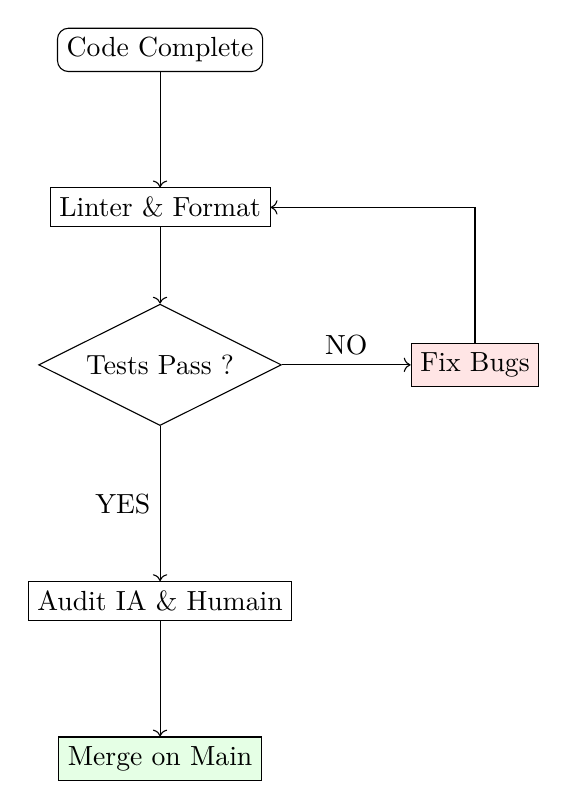
\begin{tikzpicture}[node distance=2cm]
        \node (code) [draw, rounded corners] {Code Complete};
        \node (lint) [draw, rectangle, below of=code] {Linter \& Format};
        \node (test) [draw, diamond, aspect=2, below of=lint] {Tests Pass ?};
        \node (audit) [draw, rectangle, below of=test, yshift=-1cm] {Audit IA \& Humain};
        \node (merge) [draw, rectangle, fill=green!10, below of=audit] {Merge on Main};
        \node (fix) [draw, rectangle, fill=red!10, right of=test, xshift=2cm] {Fix Bugs};

        \draw[->] (code) -- (lint);
        \draw[->] (lint) -- (test);
        \draw[->] (test) -- node[left] {YES} (audit);
        \draw[->] (test) -- node[above] {NO} (fix);
        \draw[->] (fix) |- (lint);
        \draw[->] (audit) -- (merge);
    \end{tikzpicture}
    \caption{Pipeline de Validation Qualité}
\end{figure}

\chapter{REFERENCES \& BIBLIOGRAPHIE}
\label{ann:references}

\section{Documentation Technique}
\begin{itemize}
    \item Solana Docs : \url{https://docs.solana.com}
    \item Anchor Framework : \url{https://www.anchor-lang.com}
    \item OtterSec Blog : \url{https://osec.io/blog}
\end{itemize}

\section{Rapports de l'Industrie}
\begin{itemize}
    \item Electric Capital Developer Report (2024)
    \item Messari State of Solana (Q4 2024)
    \item Solana Whitepaper (2017) : Proof of History.
    \item The Rust Book : Steve Klabnik \& Carol Nichols.
\end{itemize}

\section{Rapports de Marché}
\begin{itemize}
    \item HackerOne Security Report.
    \item Superteam Earn Metrics.
\end{itemize}

\section{Outils Cités}
\begin{itemize}
    \item Helius : Observabilité Solana.
    \item Trident : Solana Fuzzing Framework.
    \item Metaplex : Standard NFT.
\end{itemize}

\chapter{REFERENCES \& BIBLIOGRAPHIE}
\label{ann:references}

\section{Documentation Technique}
\begin{itemize}
    \item Solana Docs : \url{https://docs.solana.com}
    \item Anchor Framework : \url{https://www.anchor-lang.com}
    \item OtterSec Blog : \url{https://osec.io/blog}
\end{itemize}

\section{Rapports de l'Industrie}
\begin{itemize}
    \item Electric Capital Developer Report (2024)
    \item Messari State of Solana (Q4 2024)
    \item Solana Whitepaper (2017) : Proof of History.
    \item The Rust Book : Steve Klabnik \& Carol Nichols.
\end{itemize}

\section{Rapports de Marché}
\begin{itemize}
    \item HackerOne Security Report.
    \item Superteam Earn Metrics.
\end{itemize}

\section{Outils Cités}
\begin{itemize}
    \item Helius : Observabilité Solana.
    \item Trident : Solana Fuzzing Framework.
    \item Metaplex : Standard NFT.
\end{itemize}


\end{document}
